%%%%%%%%%%%%%%%%%%%%%%%%%%%%%%%%%%%%%%%%%%%%%%%%%%%%%%%%%%%%%%%%%%%%%%%%%%%%%%%%
%% Plantilla de memoria en LaTeX para la ETSIT - Universidad Rey Juan Carlos
%%
%% Por Gregorio Robles <grex arroba gsyc.urjc.es>
%%     Grupo de Sistemas y Comunicaciones
%%     Escuela T�cnica Superior de Ingenieros de Telecomunicaci�n
%%     Universidad Rey Juan Carlos
%% (muchas ideas tomadas de Internet, colegas del GSyC, antiguos alumnos...
%%  etc. Muchas gracias a todos)
%%
%% La �ltima versi�n de esta plantilla est� siempre disponible en:
%%     https://github.com/gregoriorobles/plantilla-memoria
%%
%% Para obtener PDF, ejecuta en la shell:
%%   make
%% (las im�genes deben ir en PNG o JPG)

%%%%%%%%%%%%%%%%%%%%%%%%%%%%%%%%%%%%%%%%%%%%%%%%%%%%%%%%%%%%%%%%%%%%%%%%%%%%%%%%

\documentclass[a4paper, 12pt]{book}
%\usepackage[T1]{fontenc}
\setcounter{tocdepth}{4}
 \setlength{\parskip}{8pt}
\usepackage{pdfpages}
\usepackage{graphicx}
\usepackage{subfig}
\usepackage[a4paper, left=2.5cm, right=2.5cm, top=3cm, bottom=3cm]{geometry}
\usepackage{times}
\usepackage[latin1]{inputenc}
\usepackage[spanish]{babel} % Comenta esta l�nea si tu memoria es en ingl�s
\usepackage{url}
%\usepackage[dvipdfm]{graphicx}
\usepackage{graphicx}
\usepackage{float}  %% H para posicionar figuras
\usepackage[nottoc, notlot, notlof, notindex]{tocbibind} %% Opciones de �ndice
\usepackage{latexsym}  %% Logo LaTeX

\title{Memoria del Proyecto}
\author{Sara L\'opez Zambrano}

\renewcommand{\baselinestretch}{1.5}  %% Interlineado

\begin{document}

\renewcommand{\refname}{Bibliograf\'ia}  %% Renombrando
\renewcommand{\appendixname}{Ap\'endice}

%%%%%%%%%%%%%%%%%%%%%%%%%%%%%%%%%%%%%%%%%%%%%%%%%%%%%%%%%%%%%%%%%%%%%%%%%%%%%%%%
% PORTADA

\begin{titlepage}
\begin{center}
\begin{tabular}[c]{c c}
%\includegraphics[bb=0 0 194 352, scale=0.25]{logo} &

\includegraphics[scale=0.25]{img/logo_vect.png} &
\begin{tabular}[b]{l}
\Huge
\textsf{UNIVERSIDAD} \\
\Huge
\textsf{REY JUAN CARLOS} \\
\end{tabular}
\\
\end{tabular}

\vspace{3cm}

\Large
INGENIER\'IA EN SISTEMAS DE TELECOMUNICACI\'ON

\vspace{0.4cm}

\large
Curso Acad\'emico 2017/2018

\vspace{0.8cm}

Trabajo Fin de Grado

\vspace{2.5cm}

\LARGE
Dise\~no e implementaci\'on de una aplicaci\'on movil h\'ibrida para la planificaci\'on de eventos


\vspace{4cm}

\large
Autor : Sara L\'opez Zambrano \\
Tutor : Pedro de las Heras Quir\'os
\end{center}
\end{titlepage}

\newpage
\mbox{}
\thispagestyle{empty} % para que no se numere esta pagina


%%%%%%%%%%%%%%%%%%%%%%%%%%%%%%%%%%%%%%%%%%%%%%%%%%%%%%%%%%%%%%%%%%%%%%%%%%%%%%%%
%%%% Para firmar
\clearpage
\pagenumbering{gobble}
\chapter*{}

\vspace{-4cm}
\begin{center}
\LARGE
\textbf{Trabajo Fin de Grado}

\vspace{1cm}
\large
Dise\~no e implementaci\'on de una aplicaci\'on movil h\'ibrida para la planificaci\'on de eventos 


\vspace{1cm}
\large
\textbf{Autor :} Sara L\'opez Zambrano \\
\textbf{Tutor :} Pedro de las Heras Quir\'os

\end{center}

\vspace{1cm}
La defensa del presente Trabajo Fin de Grado se realiz\'o el d\'ia \qquad$\;\,$ de \qquad\qquad\qquad\qquad \newline de 2017, siendo calificada por el siguiente tribunal:


\vspace{0.5cm}
\textbf{Presidente:}

\vspace{1.2cm}
\textbf{Secretario:}

\vspace{1.2cm}
\textbf{Vocal:}


\vspace{1.2cm}
y habiendo obtenido la siguiente calificaci\'on:

\vspace{1cm}
\textbf{Calificaci\'on:}


\vspace{1cm}
\begin{flushright}
Fuenlabrada, a \qquad$\;\,$ de \qquad\qquad\qquad\qquad de 2017
\end{flushright}

%%%%%%%%%%%%%%%%%%%%%%%%%%%%%%%%%%%%%%%%%%%%%%%%%%%%%%%%%%%%%%%%%%%%%%%%%%%%%%%%
%%%% Dedicatoria

\chapter*{}
\pagenumbering{Roman} % para comenzar la numeracion de paginas en numeros romanos
\begin{flushright}
\textit{Dedicado a \\
mi familia}
\end{flushright}

%%%%%%%%%%%%%%%%%%%%%%%%%%%%%%%%%%%%%%%%%%%%%%%%%%%%%%%%%%%%%%%%%%%%%%%%%%%%%%%%
%%%% Agradecimientos

\chapter*{Agradecimientos}
%\addcontentsline{toc}{chapter}{Agradecimientos} % si queremos que aparezca en el �ndice
\markboth{AGRADECIMIENTOS}{AGRADECIMIENTOS} % encabezado 

El mayor agradecimiento quiero d\'arselo a mis padres. Les agradezco enormemente
todo lo que han hecho por mi tanto en esta etapa de mi vida como en todas las que he vivido. Gracias a ellos he conseguido
llegar a este momento tan importante y he logrado alcanzar ese objetivo que me habia marcado.
Muchas gracias por apoyarme en todas mis decisiones, por ayudarme en los malos momentos
y por disfrutar, igual o mas que yo, de mis logros.

Tengo que agradecer a esta etapa de mi vida el haber conocido a una persona muy especial, mi pareja. Hemos compartido 
horas y horas de estudio, nervios, malos momentos, pero sobre todo mucha felicidad de vernos conseguir acabar lo que
nos hemos propuesto.

Tambi\'en he conocido personas que me llevo conmigo para siempre, mis telequitas. Les agradezco estar ah\'i tanto en los buenos
como en los malos momentos.


%%%%%%%%%%%%%%%%%%%%%%%%%%%%%%%%%%%%%%%%%%%%%%%%%%%%%%%%%%%%%%%%%%%%%%%%%%%%%%%%
%%%% Resumen

\chapter*{Resumen}
%\addcontentsline{toc}{chapter}{Resumen} % si queremos que aparezca en el �ndice
\markboth{RESUMEN}{RESUMEN} % encabezado

Este proyecto se trata del desarrollo de una aplicaci\'on movil cuya funcionalidad principal es el recuento de votos para una determinada encuesta. Tomar decisiones cuando el grupo de personas es amplio es dif\'icil. Para ayudar en estas decisiones se puede utilizar esta aplicaci\'on, que permite la creaci\'on de encuestas y los votantes pueden elegir cuando o qu\'e les viene mejor. El usuario que crea la encuesta, podr\'a consultar en cualquier momento cual es la opci\'on que tiene mayor n\'umero de votos y a quien pertenecen. Por ejemplo, un equipo de trabajo debe tener una reuni\'on para revisar el estado de su proyecto, pero hay que tener en cuenta la disponibilidad de todos. Una manera f\'acil de acordar una fecha y hora, en la que todos puedan, es utilizar esta aplicaci\'on para crear una encuesta con una serie de posibilidades que despu\'es podr\'an ser votadas por el equipo.

Este proyecto se ha llevado a cabo utilizando una serie de \emph{frameworks} muy utilizados hoy en d\'ia como es Angular, para la parte de \emph{frontend}. Bas\'andose en las b\'usquedas de Google, Angular es uno de los \emph{frameworks} que dominan el mercado. El aprendizaje de esta tecnolog\'ia es el principal motivo de la realizaci\'on de este proyecto, aparte de mi gran inter\'es en el desarrollo web. La parte \emph{backend} esta desarrollada con el framework Express. Este est\'a basado en Node.js que tambi\'en es muy utilizado.

Para la realizaci\'on del desarrollo, aparte de los \emph{frameworks} mencionados, ha sido necesario el aprendizaje de JavaScript, TypeScript, Node.js, HTML5, CSS3, HTTP y MongoDB.

Una vez finalizada la implementaci\'on de la aplicaci\'on y realizado un despliegue utilizando el PC como servidor, se ha procedido con la realizaci\'on de una prueba de validaci\'on basada en la utilizaci\'on de esta aplicaci\'on por usuarios que han instalado el apk en sus dispositivos m\'oviles. Tras usar la aplicaci\'on dichos usuarios se han sometido a una encuesta. La finalidad de esta, como de cualquier aplicaci\'on, es conocer posibles mejoras de cara a futuras versiones y saber como de \'util parece a los usuarios.





%%%%%%%%%%%%%%%%%%%%%%%%%%%%%%%%%%%%%%%%%%%%%%%%%%%%%%%%%%%%%%%%%%%%%%%%%%%%%%%%
%%%%%%%%%%%%%%%%%%%%%%%%%%%%%%%%%%%%%%%%%%%%%%%%%%%%%%%%%%%%%%%%%%%%%%%%%%%%%%%%
% �NDICES %
%%%%%%%%%%%%%%%%%%%%%%%%%%%%%%%%%%%%%%%%%%%%%%%%%%%%%%%%%%%%%%%%%%%%%%%%%%%%%%%%

% Las buenas noticias es que los �ndices se generan autom�ticamente.
% Lo �nico que tienes que hacer es elegir cu�les quieren que se generen,
% y comentar/descomentar esa instrucci�n de LaTeX.

%%%% �ndice de contenidos

\tableofcontents 
%%%% �ndice de figuras
\cleardoublepage
%\addcontentsline{toc}{chapter}{Lista de figuras} % para que aparezca en el indice de contenidos
\listoffigures % indice de figuras
%%%% �ndice de tablas
%\cleardoublepage
%\addcontentsline{toc}{chapter}{Lista de tablas} % para que aparezca en el indice de contenidos
%\listoftables % indice de tablas


%%%%%%%%%%%%%%%%%%%%%%%%%%%%%%%%%%%%%%%%%%%%%%%%%%%%%%%%%%%%%%%%%%%%%%%%%%%%%%%%
%%%%%%%%%%%%%%%%%%%%%%%%%%%%%%%%%%%%%%%%%%%%%%%%%%%%%%%%%%%%%%%%%%%%%%%%%%%%%%%%
% INTRODUCCI�N %
%%%%%%%%%%%%%%%%%%%%%%%%%%%%%%%%%%%%%%%%%%%%%%%%%%%%%%%%%%%%%%%%%%%%%%%%%%%%%%%%

\cleardoublepage
\chapter{Introducci\'on}
\label{sec:intro} % etiqueta para poder referenciar luego en el texto con ~\ref{sec:intro}
\pagenumbering{arabic} % para empezar la numeraci�n de p�gina con n�meros

En poco tiempo se ha producido un gran avance en el mundo de las tecnolog\'ias y en concreto
en los dispositivos m\'oviles. Tanto ha sido as\'i que estamos al alcance de la mayor\'ia de las
cosas solo disponiendo de un dispositivo m\'ovil con conexi\'on a Internet. Si navegamos en el
tiempo, desde dispositivos que s\'olo nos ofrec\'ian la capacidad de mantener una comunicaci\'on
instant\'anea entre dos personas, hemos llegado a incluso poder realizar pagos. Pero es tan importante
la evoluci\'on a nivel de dispositivo como a nivel de aplicaciones. Se han desarrollado
aplicaciones muy potentes que nos facilitan la vida. Un claro ejemplo es el poder gestionar tus
cuentas del banco y realizar operaciones desde cualquier lugar. Existen aplicaciones
para todos los gustos, necesidades e intereses.

La oferta en cuanto a desarrollo de aplicaciones m\'oviles ha ido aumentando conforme los h\'abitos de consumo se han ido dirigiendo hacia el incremento de la utilizaci\'on de dispositivos m\'oviles. Y es que el estilo de vida que impera en estos momentos, definido por la movilidad y la falta de tiempo, hace que aparatos como tablets o m\'oviles sean mucho m\'as importantes al poderse llevar sin problemas de un lado a otro.

Encontrar un d\'ia y una hora para quedar entre varias personas nunca ha sido f\'acil. Gracias a Internet y a las nuevas tecnolog\'ias ya no hay excusas. Existen en la red unas herramientas web llamadas planificadores online que nos permiten encontrar las mejores fechas y horas para organizar una cita, ya sea f\'isica o virtual.

\section{Historia de la web}
\label{sec:seccion}

La historia de la web\cite{Historia} abarca ya m\'as de 25 a\~nos, en los que se han alternado per\'iodos de intenso desarrollo con otros de estancamiento. El primer servidor de p\'aginas web de la historia se puso en marcha en diciembre de 1990. El inventor de la web, Tim Berners-Lee, pretend\'ia crear un sistema que permitiera a los investigadores del CERN compartir f\'acilmente la informaci\'on. La primera versi\'on del lenguaje de marcas inventado por Berners-Lee nunca fue publicado como documento oficial, pero si lo hubiera sido se hubiera llamado HTML 1.0.

Los investigadores del CERN,  diseminaron en sus universidades de origen el sistema creado por Berners-Lee, puesto que se trataba de un sistema abierto y libre. En aquella \'epoca ya exist\'ia Internet, pero su acceso estaba limitado principalmente a Universidades y centros de investigaci\'on.

En noviembre de 1993 se public\'o la versi\'on 1.0 de Mosaic, un navegador creado en la Universidad de Illinois por Marc Andreessen y que superaba a todos al permitir, por ejemplo, incluir im\'agenes en las p\'aginas web.

En 1994 se permiti\'o el acceso de particulares y empresas a Internet. La web se convirti\'o enseguida en el servicio m\'as empleado para ofrecer informaci\'on. La web empez\'o a verse como una gigantesca oportunidad de negocio y Marc Andreessen dej\'o la universidad para fundar Netscape, que publicar\'ia la versi\'on 1.0 de su navegador en diciembre de 1994.

En octubre de 1994 Berners-Lee fund\'o el World Wide Web Consortium (W3C), el W3C est\'a organizado en grupos de trabajo. Los primeros grupos de trabajo que se crearon se dedicaron al HTML y a las CSS.

En 1995 Microsoft incluy\'o en Windows un navegador, Internet Explorer, que poco a poco comenz\'o a crecer en el mercado en detrimento de Netscape. Entre 1995 y 2000 Microsoft y Netscape publicaron nuevas versiones cada a\~no. Para diferenciar sus productos, cada navegador fue incorporando nuevas etiquetas, lo que supuso un riesgo de fragmentaci\'on de la web.

En esos a\~nos, el W3C tambi\'en public\'o recomendaciones a ritmo fren\'etico. Por un lado, para consensuar un HTML com\'un para todos los navegadores. Pero por otro lado, proponiendo innovaciones muy importantes, como la separaci\'on entre contenido y presentaci\'on mediante hojas de estilo (CSS).

En 1995 Brian Eitch cre\'o para Netscape 2.0 el lenguaje de programaci\'on Javascript, cuyos programas se pod\'ian incluir directamente en las p\'aginas web para ser ejecutados por el navegador. Microsoft cre\'o su propia variante parcialmente incompatible. La normalizaci\'on de Javascript la llev\'o a cabo la organizaci\'on ECMA, que en 1997 empez\'o a publicar normas para unificar y desarrollar el lenguaje.

Ante la necesidad por incluir nuevos campos el W3C cre\'o el XML. El problema era que el HTML no cumpl\'ia las nuevas reglas del XML y el W3C plante\'o reformular el HTML de acuerdo con ellas (ese nuevo lenguaje se llamar\'ia XHTML).

En 1998 Netscape cre\'o la organizaci\'on Mozilla.

En el a\~no 2000 la guerra de navegadores culmin\'o con la victoria de Internet Explorer y la desaparici\'on de Netscape. Microsoft decidi\'o no seguir innovando y no habr\'ia nuevas versiones despu\'es de Internet Explorer 6.

Durante estos a\~nos, la organizaci\'on Mozilla desarroll\'o un nuevo navegador, Mozilla, de uso muy minoritario pero que respetaba las recomendaciones del W3C, apareciendo como una alternativa a Internet Explorer.

Debido a la competencia, Microsoft retom\'o el desarrollo de Internet Explorer. En 2004 se cre\'o tambi\'en el WHATWG (grupo formado por Mozilla, Apple y Opera), para retomar el desarrollo del HTML que el W3C hab\'ia abandonado en favor del XHTML, bajo el nombre de HTML 5.

En 2007 el W3C form\'o un grupo de trabajo sobre HTML, que trabajar\'ia conjuntamente con el WHATWG para publicar la recomendaci\'on HTML 5.

En 2009 Google public\'o su propio navegador: Google Chrome. En 2011 el W3C abandon\'o el desarrollo del XHTML y se concentr\'o en el HTML 5.

En 2011 el WHATWG abandon\'o por su parte el nombre de HTML 5 y pas\'o a denominarlo simplemente HTML, abandonando la idea de versiones en favor de una norma "l\'iquida", continuamente modificada y mejorada.

En 2013 Microsoft consigui\'o con Internet Explorer 11 cumplir de forma correcta las antiguas recomendaciones HTML 4 y CSS 2 y admitir lenguajes XML como SVG. Pero para sacar todo el partido a HTML 5, Microsoft cre\'o un nuevo navegador (Edge), que ya no estar\'a ligado a las nuevas versiones de Windows.

En estos a\~nos Google Chrome ha desbancado a Internet Explorer, entre otros motivos debido al gran uso de los tel\'efonos m\'oviles y al hecho de que los usuarios de Windows 7 no pueden usar Edge.



\section{Tecnolog\'ias para el desarrollo de aplicaciones web}
\label{sec:seccion}


\subsection{HTML5}
\label{subsec:estilo}

HTML\cite{HTML5}, que significa Lenguaje de Marcado para Hipertextos, es el elemento de construcci\'on
m\'as b\'asico de una p\'agina web y se usa para crear y representar visualmente una p\'agina web.
Determina el contenido de la p\'agina web, pero no su funcionalidad. Hiper Texto se refiere a enlaces
que conectan una p\'agina web con otra, ya sea dentro de una p\'agina web o entre diferentes
sitios web. Un lenguaje de marcado hace referencia a aquellos lenguajes que emplean etiquetas.
Estas etiquetas ya est\'an predefinidas dentro del lenguaje respectivo y contienen la informaci\'on
que ayudan a leer el texto. Su principal diferencia con los lenguajes de programaci\'on es que
\'estos \'ultimos poseen funciones aritm\'eticas o variables, mientras que los lenguajes de marcado
no.

HTML5 es la quinta revisi\'on del est\'andar que fue creado en 1990 y su versi\'on definitiva se
public\'o en octubre de 2014. Con HTML5, los navegadores como Firefox, Chrome, Explorer,
Safari y m\'as pueden saber c\'omo mostrar una determinada p\'agina web, saber d\'onde est\'an los
elementos, d\'onde poner las im\'agenes, d\'onde ubicar el texto.

En HTML5, se han tomado en cuenta mejoras en la creaci\'on de la estructura del c\'odigo web
y en el manejo \'optimo de las etiquetas web. De esta manera, se convierte en un est\'andar mucho
m\'as vers\'atil, que permitir\'a realizar una interacci\'on mucho m\'as poderosa y simple, mejorando
la experiencia de uso por parte del usuario y facilitando la depuraci\'on del c\'odigo web.

Las ventajas principales de esta versi\'on son:

\begin{itemize}
  \item Nueva estructura de etiquetas: permite separar el encabezado, la barra de navegacion, secciones de la p\'agina, textos, di\'alogos y el pi\'e de p\'agina.
 \item Introduccion de etiquetas video y audio: por medio de las etiquetas <video> y <audio> de HTML5, ahora puedes a\~nadir videos o audio sin necesidad de usar Adobe Flash o cualquier otro plugin de tercero. Toda la acci\'on sucede desde el propio navegador, lo que puede ayudar a disminuir al tama\~no del archivo final de tu p\'agina. 
 \item Geolocalizaci\'on: permite al sitio detectar la ubicaci\'on de cada usuario que ingresa al sitioweb.
 \item Aplicaciones web: desarrollar aplicaciones HTML5 tiene la ventaja de que el resultado final es completamente accesible, es decir, se puede acceder a esta aplicaci\'on desde un ordenador, tablet o m\'ovil.
 \item Capacidad de realizar ejecucciones offline: esto permite realizar aplicaciones de escritorio.
 \item Canvas: nueva etiqueta de dibujo sobre la p\'agina web.

\end{itemize}

\subsection{JavaScript}
\label{subsec:estilo}

JavaScript\cite{JavaScript} es un lenguaje de programaci\'on que se utiliza principalmente para crear p\'aginas
web din\'amicas. Una p\'agina web din\'amica es aquella que incorpora efectos como texto que
aparece y desaparece, animaciones, acciones que se activan al pulsar botones y ventanas con
mensajes de aviso al usuario.

Surgi\'o por la necesidad de ampliar las posibilidades del HTML. En efecto, al poco tiempo
de que las p\'aginas web apareciesen, se hizo patente que se necesitaba algo m\'as que las limitadas
prestaciones del lenguaje b\'asico, ya que el HTML solamente provee de elementos que actuan
exclusivamente sobre el texto y su estilo, pero no permite, como ejemplo sencillo, ni siquiera
abrir una nueva ventana o emitir un mensaje de aviso. La temprana aparici\'on de este lenguaje,
es posiblemente la causa de que se haya convertido en un est\'andar soportado por todos los
navegadores actuales.

Los documentos HTML permiten incrustar fragmentos de c\'odigo JavaScript, bien dentro
del propio archivo HTML o bien realizando una carga de ese c\'odigo indicando el archivo donde
se encuentra el c\'odigo JavaScript. Dentro de un documento HTML puede haber ninguno, uno o
varios scripts de JavaScript.

Adem\'as, tambien es utilizado del lado del servidor, ya que tiene la ventaja de poseer un
excelente modelo de eventos, ideal para la programaci\'on as\'incrona.


\subsection{TypeScript}
\label{subsec:typescript}

TypeScript\cite{TypeScript} es un lenguaje de programaci\'on de alto nivel que implementa muchos de los
mecanismos m\'as habituales de la programaci\'on orientada a objetos, pudiendo extraer grandes
beneficios que ser\'an especialmente deseables en aplicaciones grandes, capaces de escalar correctamente
durante todo su tiempo de mantenimiento. Puede ser usado para desarrollar aplicaciones
JavaScript que se ejecutar\'an en el lado del cliente o del servidor (Node.js).

TypeScript convierte su c\'odigo en Javascript com\'un. Es llamado tambi\'en Superset de Javascript,
lo que significa que si el navegador est\'a basado en Javascript, este nunca llegar\'a a saber que el
c\'odigo original fue realizado con TypeScript y ejecutar\'a el Javascript como lenguaje original.


\subsubsection{Ventajas}
\label{subsec:ventajas}

Las principales ventajas con respecto a JavaScript son:

\begin{itemize}
  \item Tipado est\'atico: permite mejorar el soporte y la deteccion de errores sin necesidad de arrancar el c\'odigo. Los tipos b\'asicos son: boolean, number, Any y void.
\item Gen\'ericos: muy \'utiles para hacer c\'odigo mas reusable, especialmente en listas y Arrays.
\item \emph{decorator}s: anotaciones que modifican comportamientos a nivel de clase, propiedad, m\'etodo o par\'ametro.

\end{itemize}

\subsubsection{Compilaci\'on a JavaScript}
\label{subsec:compilacion}

Para compilar a JavaScript se puede elegir el target al que queremos compilar, es decir, elegir entre ES5 o ES6.

TypeScript nos permite utilizar codigo JavaScript, lo que nos permite aprovechar un c\'odigo ya existente, incluso tiparlo mediante ficheros *.ts para TypeScript.

Tiene la capacidad de concatenar varios ficheros en uno. Tambi\'on ofrece la posibilidad de generar sourcemaps lo cual nos mapea el c\'odigo compilado a ficheros sin compilar para que haga el proceso de debuguear mas sencillo. Por \'utimo a\~nadir que genera un c\'odigo modular.

\subsection{CSS3}
\label{subsec:estilo}

CSS3 \cite{Css3} es el lenguaje utilizado para describir la presentaci\'on de documentos HTML o XML. Al
crear una p\'agina web, se utiliza en primer lugar el lenguaje HTML/XHTML para marcar los
contenidos, es decir, para designar la funci\'on de cada elemento dentro de la p\'agina y una vez
creados los contenidos, se utiliza el lenguaje CSS para definir el aspecto de cada elemento.

El objetivo inicial de CSS, separar el contenido de la forma, se cumpli\'o ya con las primeras
especificaciones del lenguaje. Sin embargo, el objetivo de ofrecer un control total a los dise\~nadores
sobre los elementos de la p\'agina ha sido m\'as dif\'icil de cubrir. Las especificaciones anteriores
del lenguaje ten\'ian muchas utilidades para aplicar estilos a las webs, pero los desarrolladores
aun contin\'uan usando trucos diversos para conseguir efectos tan comunes o tan deseados como
los bordes redondeados o el sombreado de elementos en la p\'agina.


\subsection{Sass}
\label{subsec:estilo}

Sass \cite{Sass}  es un metalenguaje de Hojas de Estilo en Cascada (CSS). Es un lenguaje de script que
es traducido a CSS.

Extiende CSS proveyendo de varios mecanismos que est\'an presentes en los lenguajes de
programaci\'on tradicionales, particularmente lenguajes orientados a objetos, pero \'este no est\'a
disponible para CSS3 como tal. Cuando SassScript se interpreta, \'este crea bloques de reglas CSS
para varios selectores que est\'an definidos en el fichero SASS. El int\'erprete de SASS traduce
SassScript en CSS.

Sass permite la definici\'on de variables de tipo number, string, colores y booleanos. Otra
ventaja es que soporta mixins Un mixin es una secci\'on de c\'odigo que contiene c\'odigo Sass.
Cada vez que se llama un mixin en el proceso de conversi\'on el contenido del mismo es insertado
en el lugar de la llamada. Los mixin permiten una soluci\'on limpia a las repeticiones de c\'odigo,
as\'i como una forma f\'acil de alterar el mismo.


\subsection{Angular}
\label{subsec:estilo}

Angular\cite{Angular} es un framework de desarrollo para JavaScript creado por Google. La finalidad de Angular es facilitar el desarrollo de aplicaciones web SPA y adem\'as proporcionar herramientas para trabajar con los elementos de una web de una manera m\'as sencilla y \'optima. Una aplicaci\'on web SPA creada con Angular es una web de una sola p\'agina, en la cual la navegaci\'on entre secciones y p\'aginas de la aplicaci\'on, as\'i como la carga de datos, se realiza de manera din\'amica, casi instant\'anea, as\'incronamente haciendo llamadas al servidor (\emph{backend} con un API REST) y sobre todo sin refrescar la p\'agina en ning\'un momento. Es decir las aplicaciones web que podemos hacer con Angular son reactivas y no recargan el navegador, todo es muy din\'amico y as\'incrono con ajax.

Los fundamentos de Angular son: 

\begin{itemize}
  \item Web components: 

	Es una API estandar para crear componentes. Tiene cuatros partes principales: las templates son bloques de html optimizados para ser reusados, HTML \emph{imports} permite la carga de dependencias de la forma mas optima posible, \emph{Custom Elements} permite definir tabs propios para HTML5 con su propio ciclo de vida y su l\'ogica y \emph{Shadow DOM} que se centra en modulorizar el DOM, esto da la ventaja de modularizar el CSS y evitar conflictos entre distintas reglas del CSS.

\item Programaci\'on reactiva:

La programaci\'on reactiva es un nuevo paradigma orientado a programar basado en flujos de datos que son los encargados de transmitir los cambios a nuestra aplicaci\'on. Con este nuevo paradigma se intenta simplificar la arquitectura de las aplicaciones y centrarlo m\'as en el uso real de la aplicaci\'on: responder a eventos, tareas as\'incronas y flujos con esas tareas as\'incronas, etc.

En Angular esto se puede llevar a cabo con la librer\'ia RxJS. Dicha librer\'ia es una enorme cantidad de clases y m\'etodos para poder hacer que toda la programaci\'on que se ha venido haciendo, se pueda manejar de manera reactiva basada en Observables de manera f\'acil.

\item ES6:

Es el est\'andar que sigue JavaScript desde junio de 2015. 

Contiene algunas novedades como: clases e interfaces, variables y constantes, arrow functions, promises, definici\'on de m\'odulos, iteradores, etc.

\item TypeScript:

Como se ha explicado m\'as detalladamente en en apartado \ref{subsec:typescript}, es m\'as interesante que el uso de JavaScript ya que permite tipado est\'atico, hacer gen\'ericos y \emph{decorators}.

\end{itemize}

\subsubsection{Funcionalidades}
\label{subsec:func_angular}

\begin{itemize}
  \item Modularizaci\'on

	La filosof\'ia de Angular empuja hacia que todo sea modular. Se crea una clase, se exporta y ya est\'a disponible para ser importada en otro componente o en otra parte de la aplicaci\'on y ser reutilizada. La propia libreria de Angular est\'a modularizada.

  \item Componentes

Pieza de c\'odigo que controla una parte de la vista. No es nada m\'as que una clase de ES6 a\~nadiendole un \emph{decorator} de TypeScript  llamado Component. Esto permite transformar esta clase en un web component con un nombre de selector y una template. La template puede crearse en un fichero aparte para que la organizaci\'on del c\'odigo sea buena.

Una aplicaci\'on en si de Angular es un componente, que contiene subcomponentes.

Angular tiene un ciclo de vida para componentes y directivas, como son: ngOnChanges, ngOnInit, ngDoCheck, ngAfterContetInit, ngAfterContentChecked, ngAfterViewInit, etc.

   \item Templates

En esta parte se crean los bloques de la sintaxis de HTML. Acepta todas las tags de HTML5 menos script, no puede embeber c\'odigo JavaScript dentro de la template.

Las etiquetas de HTML se pueden potenciar con las directivas de Angular.

Toda la l\'ogica que se ejecute en el template esta siendo ejecutado en el \emph{scope} del componente al que pertenece.

\item Bindeo de datos

El bindeo es de una sola direcci\'on. Los distintos tipos de bindeo que existen son del componente hacia el DOM, para mostrar valores en la vista, para pasarselo a otras templates como par\'ametro, y del DOM al componentes, para enviarle los eventos.

\item Inyecci\'on

Usa la inyecci\'on de dependencias para los servicios. Un servicio es una clase de ES6 que contiene un \emph{decorator} llamado Injectable. De esta forma esta clase puede ser inyectada en cualquier parte de la aplicaci\'on. Adem\'as es necesario incluirlo como \emph{provider} de forma que sepa de esta dependencia la aplicaci\'on.

Para inyectar, se hace a trav\'es del constructor.

\item Routing

Angular tiene su propio componente de rutas y navegaci\'on entre vistas. Es un servicio opcional y no forma parte del \emph{core} de Angular. 

Interpreta las URL como una instrucci\'on de navegaci\'on a un componente o vista. Opcionalmente puede pasar par\'ametros.

\item Detecci\'on de cambios

Angular crea por cada componente un detector de cambios en tiempo de ejecici\'on adaptado a la estructura concreta de cada uno de ellos. Esto permite una gran optimizaci\'on de dichos detectores de cambios.

\end{itemize}


\subsubsection{Arquitectura}
\label{subsec:arquitectura_angular}

\begin{figure}[H]
  \centering
  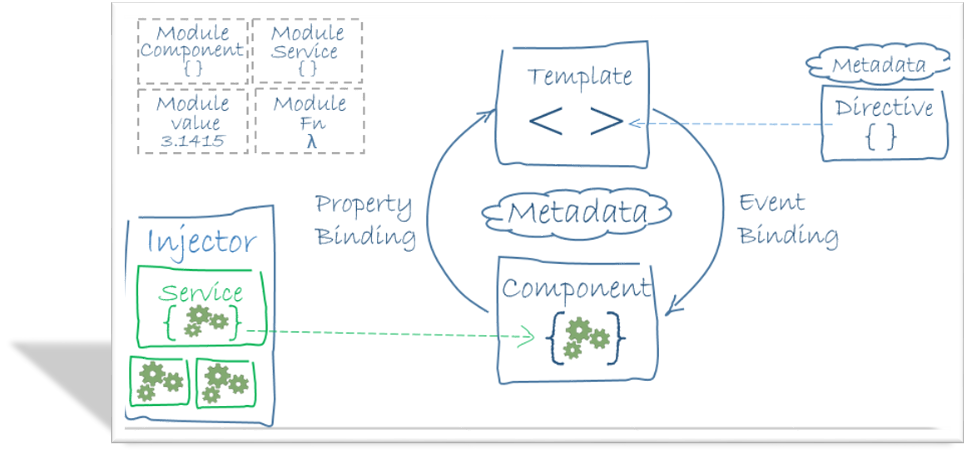
\includegraphics[width=10cm, keepaspectratio]{img/arq_angular}
  \caption{Arquitectura Angular}
  \label{figura:arq_angular}
\end{figure}


\subsection{Ionic 2}
\label{subsec:ionic}

Ionic 2\cite{Ionic} se trata de un framework destinado al desarrollo de aplicaciones h\'ibridas, aunque tambi\'en
puede ser utilizado para para implementar aplicaciones web. Una aplicaci\'on h\'ibrida es aquella
desarrollada por las tecnolog\'ias web: HTML, CSS Y JavaScript. Este tipo de aplicaciones tienen
una serie de ventajas como ser compatibles para una gran cantidad de sistemas operativos con
un tiempo de desarrollo menor, pero a cambio de esta gran ventaja el rendimiento es menor que
en una aplicaci\'on nativa.

Su caracter\'istica fundamental es que usa por debajo Angular, esto le da ventajas como tener
una buena estructura de proyecto y contar con una buena gama de componentes y directivas.

\subsubsection{Componentes}
\label{subsec:estilo}

Los componentes se utilizan unos a otros para la obtenci\'on de objetivos globales de la aplicaci\'on. Est\'an pensados para, de manera modular y encapsulada, resolver peque\~nos problemas.
Ionic ofrece componentes f\'aciles de utilizar, pero para comportamientos m\'as espec\'ificos de
nuestro modelo de negocio, ser\'a necesario crear nuestros propios componentes.

Los componentes de Ionic 2 se adaptan al dispositivo est\'eticamente. Manteniendo el mismo
c\'odigo, en un dispositivo iOS tiene diferente vista que en un dispositivo Android, ya que se
visi\'on de nativa y adem\'as da al usuario una experiencia cercana a la que est\'a acostumbrada en
su tel\'efono. Sin embargo, es decisi\'on del desarrollador mantener esta visi\'on en su aplicaci\'on o
personalizar la est\'etica a su gusto.
Se adapta al sistema operativo en el que se compila. 

\subsubsection{Apache Cordova}
\label{subsec:estilo}

Para el acceso a componentes nativos desde la aplicaci\'on de Ionic, como la c\'amara, aceler
\'ometro, teclado, usa plugins que proporciona Apache Cordova. Tambi\'en nos permite compilar
el desarrollo realizado con Ionic con tecnolog\'ias web en aplicaciones para m\'oviles instalables
mediante tiendas de aplicaciones.

\subsubsection{Estructura}
\label{subsec:estilo}

Un proyecto con Ionic contiene una lista de capetas y archivos. Cada parte tiene su funci\'on:

\begin{figure}[H]
  \centering
  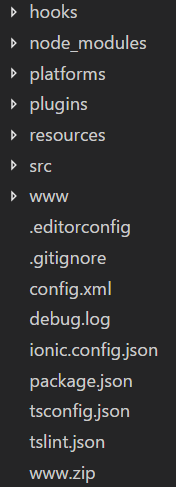
\includegraphics[width=3cm, keepaspectratio]{img/estructura_ionic}
  \caption{Estructura ionic}
  \label{figura:estructura_ionic}
\end{figure}

\begin{itemize}
  \item SRC: carpeta que contiene los archivos fuente con el c\'odigo desarrollado de la aplicaci\'on.
 \item WWW: contiene los archivos que se producen al realizar la transpilaci\'on del TypeScript y compilado de los archivos Sass, es decir, la trasformaci\'on de todos los archivos de 'src', de tal manera que el navegador sea capaz de entender.
 \item PLUGINS: contiene todos los plugins nativos que se utilizan para la aplicaci\'on.
 \item PLATFORM: archivos de cada plataforma a la que da soporte la aplicaci\'on. Suele ser Android e iOS.
 \item RESOURCES: contiene los iconos de la aplicaci\'on y el splash screen.
 \item HOOKS: scripts que se crean para ser ejecutados autom\'aticamente despu\'es de algo espec\'ifico.
\item NODE MODULES: dependencias de npm que vienen definidas en el package.json e instaladas en local dentro de tu proyecto.

\end{itemize}

\subsection{HTTP}
\label{subsec:estilo}

Son las siglas de \emph{Hypertext Transfer Protocol}\cite{HTTP}. Es un protocolo de transferencia donde se utiliza un sistema mediante el cual se permite la transferencia de informaci\'on entre diferentes servicios y los clientes que utilizan p\'aginas web.

Este protocolo opera por petici\'on y respuesta entre el cliente y el servidor. A menudo las peticiones tienen que ver con archivos, ejecuci\'on de un programa, consulta a una base de datos, traducci\'on y otras funcionalidades. Toda la informaci\'on que opera en la Web mediante este protocolo es identificada mediante el URL o direcci\'on.

La t\'ipica transacci\'on de protocolo HTTP se compone de un encabezado seguido por una l\'inea en blanco y luego un dato. Este encabezado define la acci\'on requerida por el servidor.

Una solicitud HTTP es un conjunto de l\'ineas que el navegador env\'ia al servidor. Contiene una l\'inea de solicitud que especifica el tipo de documento solicitado, el m\'etodo que se aplicar\'a y la versi\'on del protocolo utilizada. La l\'inea est\'a formada por tres elementos que deben estar separados por un espacio: el m\'etodo, la direcci\'on URL y la versi\'on del protocolo utilizada por el cliente. Tambien contiene los campos del encabezado de solicitud y el cuerpo de la solicitud.

\subsection{Servicio REST}
\label{subsec:rest}
Significa \emph{Representational State Transfer}\cite{REST}, traducido 'transferencia de representaci\'on de estado'. La clave de REST es que un servicio REST no tiene estado lo que quiere decir que, entre dos llamadas cualesquiera, el servicio pierde todos sus datos.

\subsection{Node.js}
\label{subsec:estilo}

Node.js\cite{Node} es un entorno de ejecuci\'on multiplataforma de c\'odigo abierto para desarrollar aplicaciones
web. Esta librer\'ia se ejecuta sobre JavaScript y est\'a basado en el motor V8 de Javascript
de Google. Este motor est\'a dise\~nado para correr en un navegador y ejecutar el c\'odigo de 
Javascript de una forma extremadamente r\'apida.

Se trata de un int\'erprete Javascript del lado del servidor, lo que permite utilizar el mismo
lenguaje de programaci\'on tanto para cliente como para servidor.
Node sirve para facilitar la creaci\'on de aplicaciones web escalables de manera sencilla y con
gran estabilidad, pudiendo ser utilizado para desarrollar cualquier tipo de aplicaci\'on. Adem\'as,
es importante volver a destacar su alt\'isima velocidad y su flexibilidad, dos de sus cualidades
m\'as importantes.

Trabaja con un \'unico hilo de ejecuci\'on que es el encargado de organizar todo el flujo de
trabajo que se deba realizar. Gestiona sus tareas de manera as\'incrona y para trabajar de manera
\'optima delega todo el trabajo en un poll de threads. La libreria que construye esto es Libuv, una
vez que el trabajo ha sido completado emite un evento recibido por Node.js.



\subsection{Express}
\label{subsec:express}

Express\cite{Express} es una infraestructura de aplicaciones web Node.js m\'inima y flexible que proporciona
un conjunto s\'olido de caracter\'isticas para las aplicaciones web y m\'oviles. Contiene muchos
m\'etodos de programa de utilidad HTTP y \emph{middleware}.

Node.js es una plataforma construida sobre el motor de JavaScript de Google Chrome (V8)
que permite la ejecuci\'on de JavaScript en el lado del servidor. Permite montar un servidor HTTP
utilizando el modulo http que viene incluido en el core de Node.

Para comenzar un proyecto en Express es necesario configurar en que puerto e IP va a estar
escuchando el servidor para atender a las peticiones. Adem\'as, es necesario a\~nadir las urls a las
que tiene que atender y que m\'etodo realizar para cada caso.

\subsubsection{Estructura}
\label{subsec:estilo}

\begin{figure}[H]
  \centering
  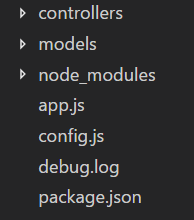
\includegraphics[width=3cm, keepaspectratio]{img/estructura_express}
  \caption{Estructura express}
  \label{figura:estructura_express}
\end{figure}


\subsection{MongoDB}
\label{subsec:estilo}

MongoDB\cite{MongoDB} se trata de una base de datos no relacional, es decir, NoSQL. Esto significa que los datos no
son almacenados en tablas y no garantiza consistencia. Este tipo de bases de datos tienen ciertas
desventajas, como: poca eficiencia en aplicaciones que necesiten usar los datos intensivamente,
o si contiene gran n\'umero de indexaciones. A cambio de esta desventaja tiene la capacidad de
manejar mucha cantidad de datos, no generan cuellos de botella y se ejecutan en clusters de
m\'aquinas baratas.

Este tipo de bases de datos surgieron por el \emph{Big Data}, donde la informaci\'on que se genera
es muy grande, de manera r\'apida y constante, y que, adem\'as, en ocasionas la forma es no
estructurada y cambiante. Las bases de datos relacionales ten\'i\'in carencias para afrontar esto.

\subsubsection{Colecciones}
\label{subsec:estilo}

MongoDB es una base de datos orientada a documentos, es decir, los documentos son almacenados
en BSON, que es una representaci\'on binaria de JSON. No siguen un esquema dijo,
los documentos de una misma colecci\'on pueden tener esquemas diferentes.

En MongoDB los documentos se agrupan en colecciones. Aunque lo normal es que los documentos
de una colecci\'on compartan estructura, puede ser flexible porque la estructura no se
impone a ning\'un documento y din\'amica porque la estructura puede cambiar. En el caso de que se
decida variar la estructura de datos, no ser\'ia necesarios crear ni modificar las colecciones, bastar\'ia con almacenar los nuevos documentos, con una estructura distinta, en la misma colecci\'on
o en otra.

No proporciona integridad referencial. Esto significa que, si en una colecci\'on hacemos referencia
a un documento de otra colecci\'on, la base de datos no tiene la responsabilidad de comprobar
que el documento referenciado existe.


\subsubsection{Velocidad}
\label{subsec:estilo}

MongoDB tiene una baja velocidad en generar o modificar informaci\'on. Esto provoca que
el acceso a la base de datos este m\'as tiempo bloqueado. Una operaci\'on de escritura bloquea el
acceso a toda la base de datos en la que se efect\'ua la operaci\'on. Para solucionar esto hay que
evitar actualizaciones que provoquen movimientos, es decir, que el crecimiento de un documento
sea tan grande que suponga un cambio de caj\'on. Cada documento se encuentra almacenado
en un caj\'on el cual cuenta con un espacio extra para posibles crecimientos futuros.

A cambio de esta baja velocidad de escritura, proporciona una gran rapidez de lectura.



\section{Trabajo relacionado}
\label{sec:relacionado}

Este proyecto esta inspirado en una aplicaci\'on similar conocida con el nombre de Doodle. Es una herramienta automatizada muy sencilla que te evita hacer varias llamadas o enviar multitud de emails o mensajes para quedar con alguien. Por lo tanto, mejora la organizaci\'on en todos los sentidos, tanto en eficiencia como en rapidez y concreci\'on.

Pero esta no es la \'unica aplicaci\'on que existe para el tema de la planificaci\'on, existen otras similares:

\begin{itemize}
  \item Timebridge\cite{Timebridge}: dirigida a profesionales. Su gran aliciente es que dispone adem\'as de soluciones para teleconferencia y reuniones en l\'inea, aunque no pueda competir con otras m\'as especializadas en ello y sean de pago. Adem\'as no requiere instalaci\'on y permite compartir archivos, acciones de pizarra, tomar notas en tiempo real de forma colaborativa, el seguimiento posterior a la reuni\'on de elementos de acci\'on y notas.
 \item When is Good\cite{WhenIsGood}: es una de las m\'as sencillas aunque no muy intuitiva y la m\'as adecuada para programar planes informales.
 \item Calendly\cite{Calendly}: se recomienda para establecer reuniones comerciales ya que funciona para encuentros cara a cara y al permitir acceder a la disponibilidad de la otra persona se pueden concertar citas de forma inmediata. 
 \item TimePal\cite{TimePal}: es una aplicaci\'on muy \'util cuando los asistentes son de diferentes husos horarios. Funciona como un tablero en el que se introducen las distintas horas en la que se est\'a disponible y muestra la hora que ser\'ia en las otras regiones. Adem\'as indica las horas del amanecer y atardecer en los distintos lugares as\'i como si es horario laboral o no.
 \item ScheduleOnce\cite{ScheduleOnce}: servicio orientado a empresas se conecta con los calendarios de Outlook, Office 365, Google, and iCloud y se puede integrar con Salesforce, Infusionsoft, GoToMeeting and WebEx.  Accedes a la p\'agina web, indicas las franjas horarias que te interesan y la herramienta crea dos enlaces: el primero se enviar\'a a los invitados, que indicaran el d\'ia y la hora que les conviene, y, el segundo, servir\'a para hacer el seguimiento de las respuestas.
\end{itemize}



\section{Estructura de la memoria}
\label{sec:estructura}

Despu\'es de esta introducci\'on, en la que hemos analizado diferentes plataformas que motivan
el desarrollo de este proyecto y ofrecido una visi\'on global del mundo web, explicando
sus or\'igenes, como ha evolucionado su desarrollo en la actualidad con tecnolog\'ias modernas
y comentando brevemente las tecnolog\'ias y herramientas utilizadas en este proyecto, continuaremos
describiendo las necesidades que han llevado a la realizaci\'on de este Trabajo Fin
de Grado. Esto se presenta en el cap\'itulo 2.

En el cap\'itulo 3 se explica el dise\~no e implementacion del proyecto. Este cap\'itulo es el m\'as extenso ya que contiene todo 
el desarrollo del proyecto. De la parte \emph{frontend} se detalla el mapa de navegac\'ion que contiene la aplicaci\'on, el dise\~no de cada pantalla con su correspondiente funcionalidad y la 
estructura de proyecto. De la parte \emph{backend} se describe la estructura de colecciones de la base de datos, los controladores utilizados, las relaciones que existen entre las colecciones y 
la seguridad.

En el cap\'itulo 4 se detalla como se ha llevado un experimento cuya finalidad es conocer la opini\'on de los usuarios sobre la aplicaci\'on, es importante
que tenga facil usabilidad.

Por \'ultimo est\'an las conclusi\'on obtenidas tras todo el aprendizaje y desarrollo del proyecto, as\'i como trabajos futuros para mejorar ciertas partes
de la aplicaci\'on.



%%%%%%%%%%%%%%%%%%%%%%%%%%%%%%%%%%%%%%%%%%%%%%%%%%%%%%%%%%%%%%%%%%%%%%%%%%%%%%%%
%%%%%%%%%%%%%%%%%%%%%%%%%%%%%%%%%%%%%%%%%%%%%%%%%%%%%%%%%%%%%%%%%%%%%%%%%%%%%%%%
% OBJETIVOS %
%%%%%%%%%%%%%%%%%%%%%%%%%%%%%%%%%%%%%%%%%%%%%%%%%%%%%%%%%%%%%%%%%%%%%%%%%%%%%%%%

\cleardoublepage % empezamos en p�gina impar
\chapter{Objetivos} % t�tulo del cap�tulo (se muestra)
\label{chap:objetivos} % identificador del cap�tulo (no se muestra, es para poder referenciarlo)

\section{Objetivo general} % t�tulo de secci�n (se muestra)
\label{sec:objetivo-general} % identificador de secci�n (no se muestra, es para poder referenciarla)

Este trabajo fin de grado consiste en crear una aplicaci\'on que ayude a tomar decisiones a la
hora de organizar eventos o reuniones, adem\'as de realizar encuestas de todo tipo.

Para organizar un nuevo evento o tomar determinada decisi\'on, un usuario debe crear una encuesta
con un determinado t\'itulo y las opciones a votar. Tambi\'en pueden a\~nadirse otros detalles opcionales. 
Una vez creada la encuesta se invita a las personas que tienen que votar por alguna o algunas
de las opciones indicadas. De esta manera se puede hacer un recuento y conocer cual es la opci\'on m\'as
votada.


\section{Objetivos espec\'ificos}
\label{sec:objetivos-especificos}

Una vez conocido cu\'al es el objetivo proncipal del proyecto, es interesante conocer cuales son los
objetivos m\'as espec\'ificos. Como este proyecto consta de dos partes, cada una de ellas cuenta
con los suyos propios. En el caso de la parte \emph{frontend} se trata de objetivos m\'as relacionados
con la parte del usuario y en el caso de \emph{backend} son objetivos relacionados con los datos
almacenados.

\subsection{Frontend}
\label{sec:objetivos-especificos}

\begin{itemize}
 \item Controlar los formatos introducidos al registrarse, de tal manera que no pueda introducirse un email con formato no v\'alido ni una contrase\~na con menos de 6 caracteres.
 \item Visi\'on global del usuario en cuanto a todas las encuestas que ha creado y poder visualizar los votos de esta.
 \item Permitir elegir el tipo de encuesta que se quiere crear. Esta elecci\'on ser\'a entre encuesta de tipo fecha o de tipo texto.
 \item Las encuestas de tipo fecha y de tipo texto unicamente se direfencian en el tipo de opci\'on que se puede a\~nadir.
 \item Dar opci\'on al usuario de a\~nadir hora y fecha o solo una fecha, en el caso de encuesta de tipo fecha.
 \item Al crear una encuesta poder elegir si se permite votar multiples \'opciones o se restringe a una sola votaci\'on por persona.
 \item Validar los campos introducidos al crear una encuesta. Los campos obligatorios son el t\'itulo y las opciones.
 \item Como datos opcionales, poder a\~nadir a la encuesta la ubicaci\'on del evento o alg\'un comentario.
 \item Un usuario s\'olo podr\'a enviar la encuesta creada a aquellos usuarios que est\'en en su lista de amigos
 \item Tr\'as realizar la votaci\'on de una encuesta, es posible modificar el voto.
 \item Un usuario puede cambiar sus datos personales de la cuenta, que son el nombre de usuario y contrase\~na.
\item Para facilitar la b\'usqueda de amigos, el usuario no deber\'a introducir el nombre concreto en el buscador, se hace una b\'usqueda de todos los nombres que contengan los caracteres introducidos.
\item Un usuario que a\'un no tenga amigos en su lista, no puede crear una encuesta.
\end{itemize}

\subsection{Backend}
\label{sec:objetivos-especificos}

\begin{itemize}
 \item S\'olo puede haber un nombre de usuario y email registrado en la aplicaci\'on.
 \item Encriptar las contrase\~nas que se han registrado y as\'i guardarlas en la base de datos.
 \item Permitir el cambio de nombre de usuario o contrase\~na, siempre que el usuario introduzca una contrase\~na v\'alida.
 \item Est\'a permitido borrar una cuenta, pero solo podr\'a eliminarla el propio usuario.
 \item Si un usuario vota de nuevo una encuesta, su antigua votaci\'on queda anulada.
 \item Solo puede haber un voto por usuario y opci\'on.
 

\end{itemize}





%%%%%%%%%%%%%%%%%%%%%%%%%%%%%%%%%%%%%%%%%%%%%%%%%%%%%%%%%%%%%%%%%%%%%%%%%%%%%%%%
%%%%%%%%%%%%%%%%%%%%%%%%%%%%%%%%%%%%%%%%%%%%%%%%%%%%%%%%%%%%%%%%%%%%%%%%%%%%%%%%
% DISE�O E IMPLEMENTACI�N %
%%%%%%%%%%%%%%%%%%%%%%%%%%%%%%%%%%%%%%%%%%%%%%%%%%%%%%%%%%%%%%%%%%%%%%%%%%%%%%%%

\cleardoublepage
\chapter{Dise\~no e implementaci\'on}

\begin{figure}[H]
  \centering
  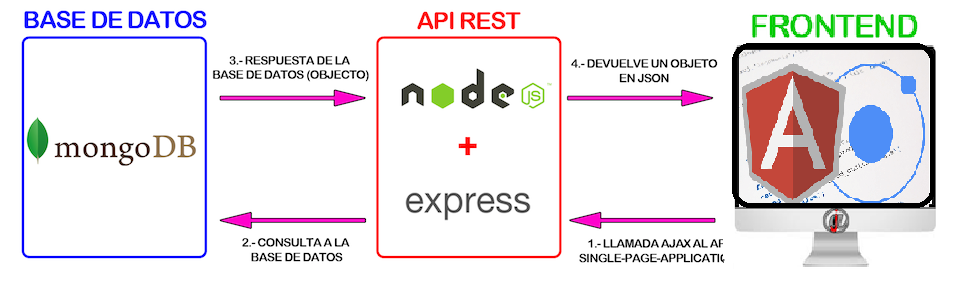
\includegraphics[width=14cm]{img/resumen.png}
  \caption{Arquitectura de la aplicaci\'on}
  \label{figura:frontend_backend}
\end{figure}


Este trabajo esta desarrollado utilizando la estructura de la figura \ref{figura:frontend_backend}, en la que podemos ver las principales tecnolog\'ias utilizadas. Este trabajo se puede
dividir en dos proyectos claramente diferenciados: la parte \emph{frontend} y la parte \emph{backend}\cite{FrontendBackend}.

Por una parte existe un proyecto desarrollado con Ionic. Como ya ha sido explicado en el apartado \ref{subsec:ionic}, es un \emph{framework} basado en Angular. Este proyecto contiene toda la funcionalidad sobre el interfaz del usuario,
es decir, la parte con la que interactua un usuario.

Por otra parte hay un proyecto desarrollado con Express, que b\'asicamente es Node.js. Este proyecto tiene la funcionalidad de tratar los datos de la aplicaci\'on, controlar su almacenamiento en la base de datos MongoDB y servir los datos
a la parte de \emph{frontend}.

Estos dos proyectos que son realizados de forma independiente tienen que ser unidos para que la 
aplicaci\'on pueda funcionar. Esta uni\'on es posible mediante llamadas AJAX, que es un mecanismo que permite la comunicaci\'on as\'incrona entre el cliente y el servidor de manera continua sin interrumpir los aspectos visuales de la p\'agina, haciendo actualizaciones parciales de la misma.
De estas llamadas, el servidor devuelven objetos JSON, esto es un formato para el intercambios de datos que puede ser le\'ido por cualquier lenguaje de programaci\'on.

A continuaci\'on son explicados los detalles en profundidad de cada uno de los proyectos, para conocer el funcionamiento de cada uno.



\section{Frontend}
\label{sec:frontend}

Es una especialidad para el desarrollo web, que trabaja la interfaz web y hace que el usuario pueda interactuar con nuestra web.
Casi todo lo se ve en la pantalla cuando se accede a una web es desarrollo \emph{frontend}, se centra en dar formato a contenidos, desarrollo del aspecto de la web y manipular resultados de datos obtenidos.

\subsection{Mapa de navegaci\'on}
\label{sec:mapa_navegacion}

El t\'ermino navegaci\'on describe la acci\'on de moverse entre las p\'aginas y dentro de la p\'agina.
Es el punto de partida de la experiencia del usuario. Es la forma en que los usuarios buscan el
contenido y las caracter\'isticas que les interesan.

Existen dos tipos de estructura de navegacion: jer\'arquica y plana. En una estructura jer\'arquica,
las p\'aginas se organizan en una estructura parecida a un \'arbol. Cada p\'agina secundaria tiene un
\'unico elemento primario, pero un elemento primario puede tener una o m\'as p\'aginas secundarias.
Para llegar a una p\'agina secundaria, hay que moverse a trav\'es del elemento primario. En el caso
de la estructura plana o lateral, las p\'aginas existen en paralelo. Puedes ir de una p\'agina a otra
en cualquier orden.

Esta aplicaci\'on sigue una estructura combinada entre jer\'arquica y plana. Se usan estructuras
planas para las p\'aginas de nivel superior que pueden verse en cualquier orden, y estructuras
jer\'arquicas para las p\'aginas que tienen relaciones m\'as complejas.

En la figura \ref{figura:mapa_navegacion} se puede ver el mapa de navegaci\'on de la aplicaci\'on. Empieza en la pantalla de login. Desde ah\'i se puede acceder al registro o a la pantalla de home si se han introducido bien los par\'ametros. Una vez en la pantalla de home, se puede acceder a cualquier parte de la aplicaci\'on.

Cada una de las dem\'as pantallas tienen su propia navegaci\'on. En el caso de Mis encuestas, se puede acceder al detalle de esta. En el caso de nueva encueta, se accede al primer paso, de este al segundo y de este al tercero. En el caso de Mis amigos, no contiene ninguna navegaci\'on aparte de la propia del Header y en el caso de Votos pendientes, de ella puedes navegar a editar votos.

La navegaci\'on del Header, tambi\'en podemos verla en la figura \ref{figura:mapa_navegacion} y esta puesta como un caso por separado, ya que es com\'un para todas las pantallas que contienen estos header. Como se puede ver, existen dos tipos de header, que ser\'an explicados con mas detalle en el apartado \ref{sec:header}.

\begin{figure}[H]
  \centering
  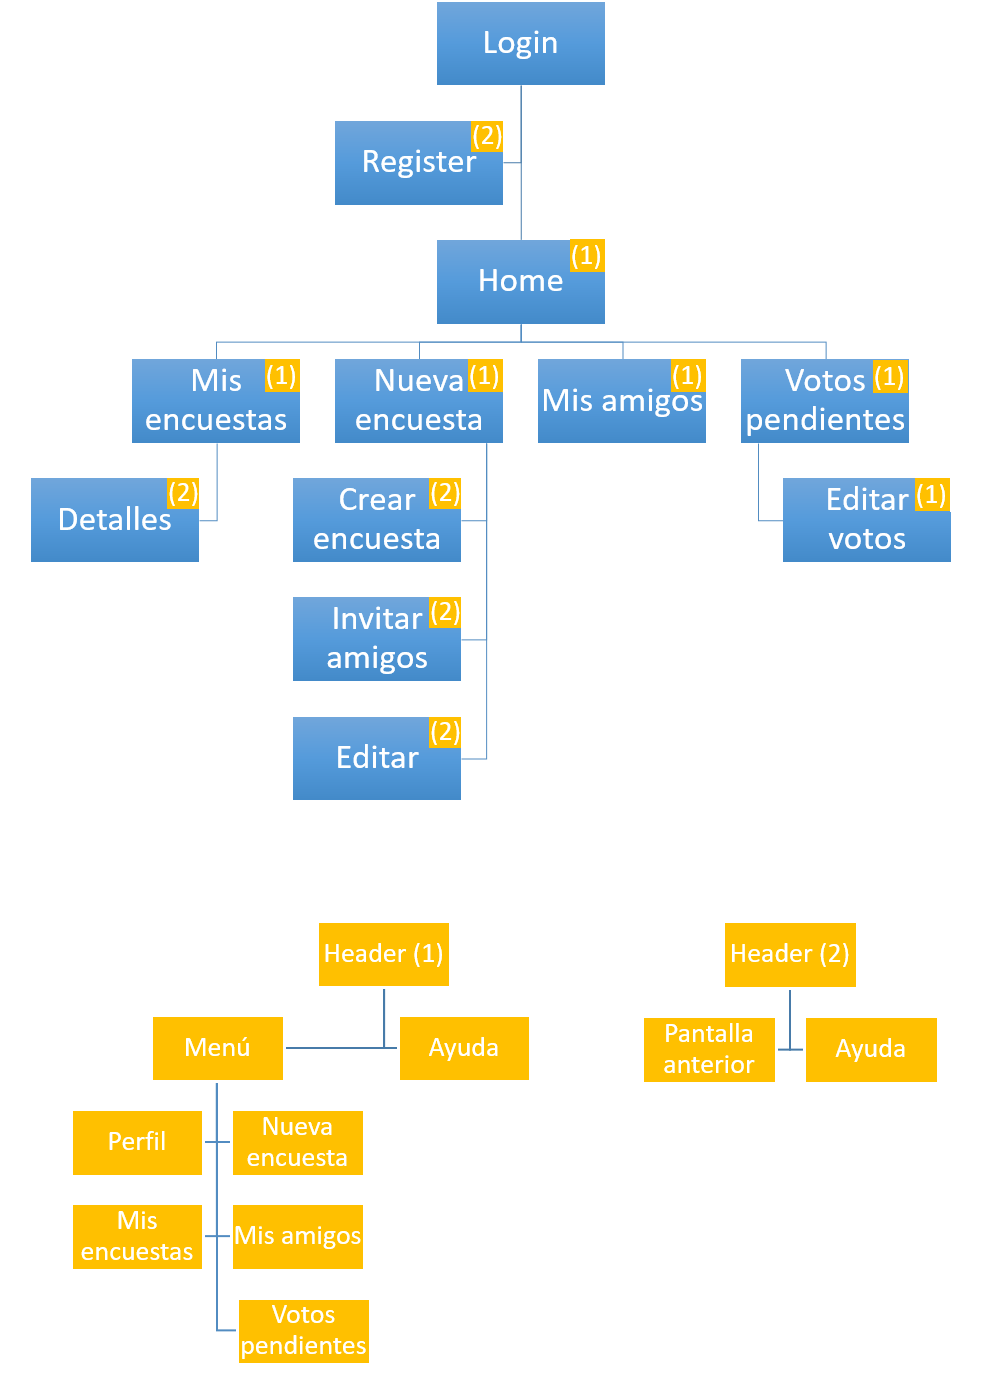
\includegraphics[width=15cm, keepaspectratio]{img/mapa_navegacion.png}
  \caption{Mapa navegaci\'on}
  \label{figura:mapa_navegacion}
\end{figure}




\subsection{Funcional}
\label{sec:funcional}

\subsubsection{Login}
\label{sec:login}

\begin{figure}[H]
 \centering
  \subfloat[Login]{
   \label{f:login}
    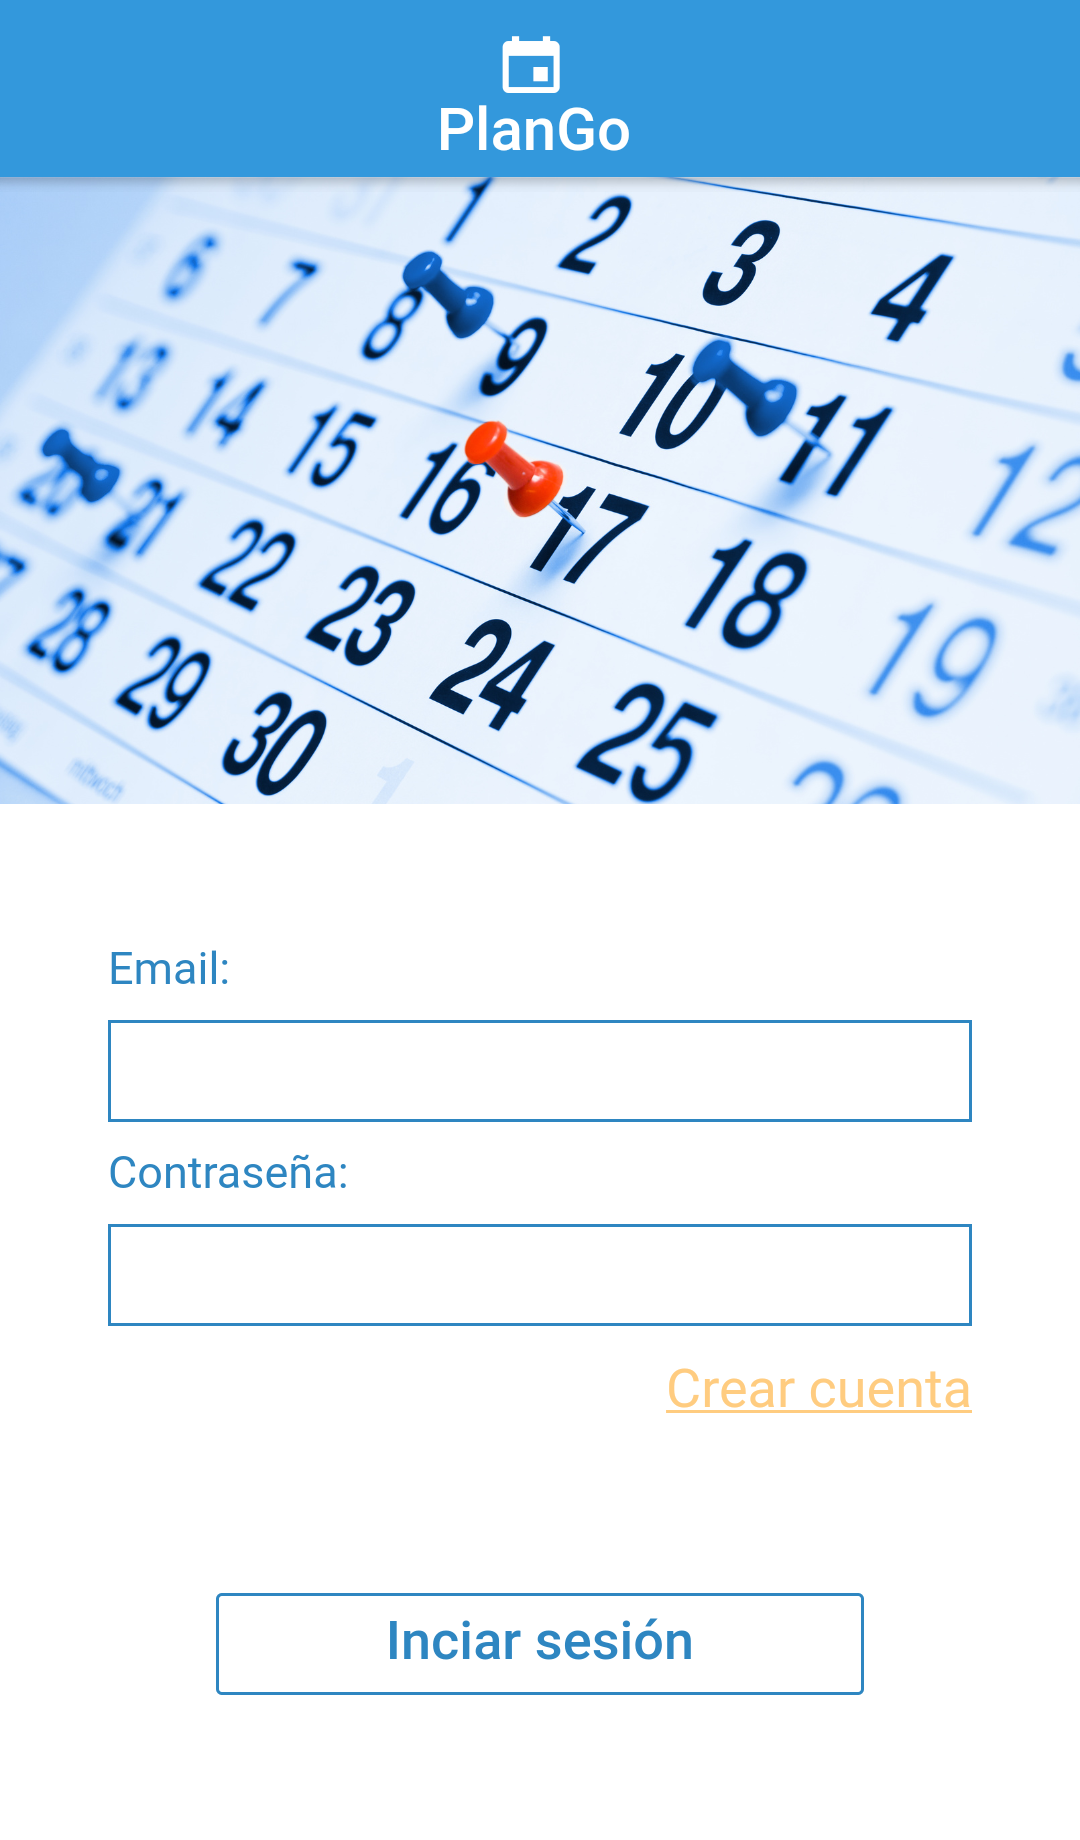
\includegraphics[width=0.3\textwidth]{img/login.png}}
  \subfloat[Error]{
   \label{f:error}
    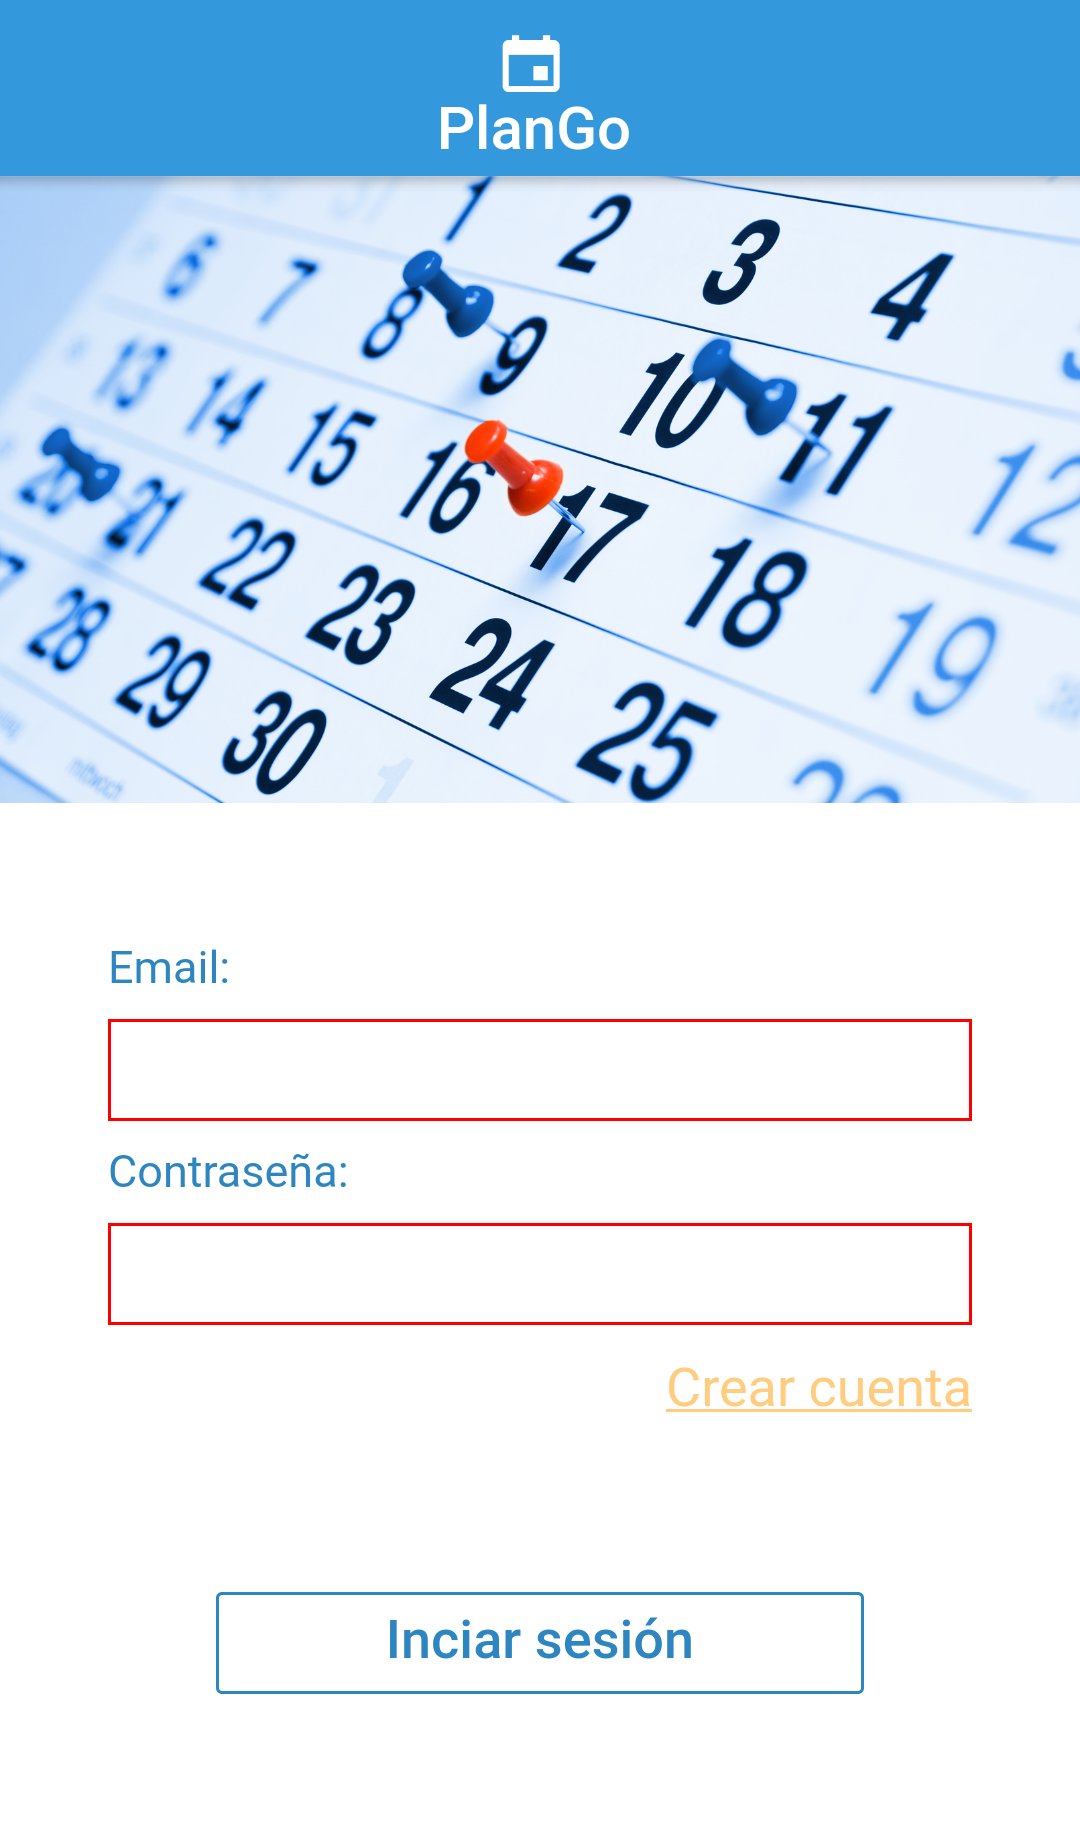
\includegraphics[width=0.3\textwidth]{img/login_error.png}}
 \caption{Pantalla de login}
 \label{f:animales}
\end{figure}

En la pantalla de login podemos encontrar dos inputs para poder introducir el correo y la
contrase\~na. De esta forma se puede comprobar si el usuario tiene cuenta en la aplicaci\'on y
adem\'as se identifica al usuario que est\'a usando la aplicaci\'on.

Se trata de un formulario reactivo, esto permite que los valores no tienen que ser recuperados
de un servidor, se pueden validar de forma inmediata. Ambos son campos requeridos por lo que
se comprueba que han sido introducidos, y en el caso de la contrase\~na que contenga m\'inimo 6
caracteres. Para el caso del email, se comprueba que sea un formato valido.

Tambi\'en encontramos un enlace para que aquellos usuarios que a\'un no han utilizado esta
aplicaci\'on puedan crearse una cuenta. Este enlace lleva a la p\'agina de registro.

Finalmente encontramos un bot\'on para iniciar sesi\'on. Al pulsar en este bot\'on se realiza la
validaci\'on del formato de email y se manda una petici\'on al servidor.


\subsubsection{Registro}
\label{sec:registro}

\begin{figure}[H]
  \centering
  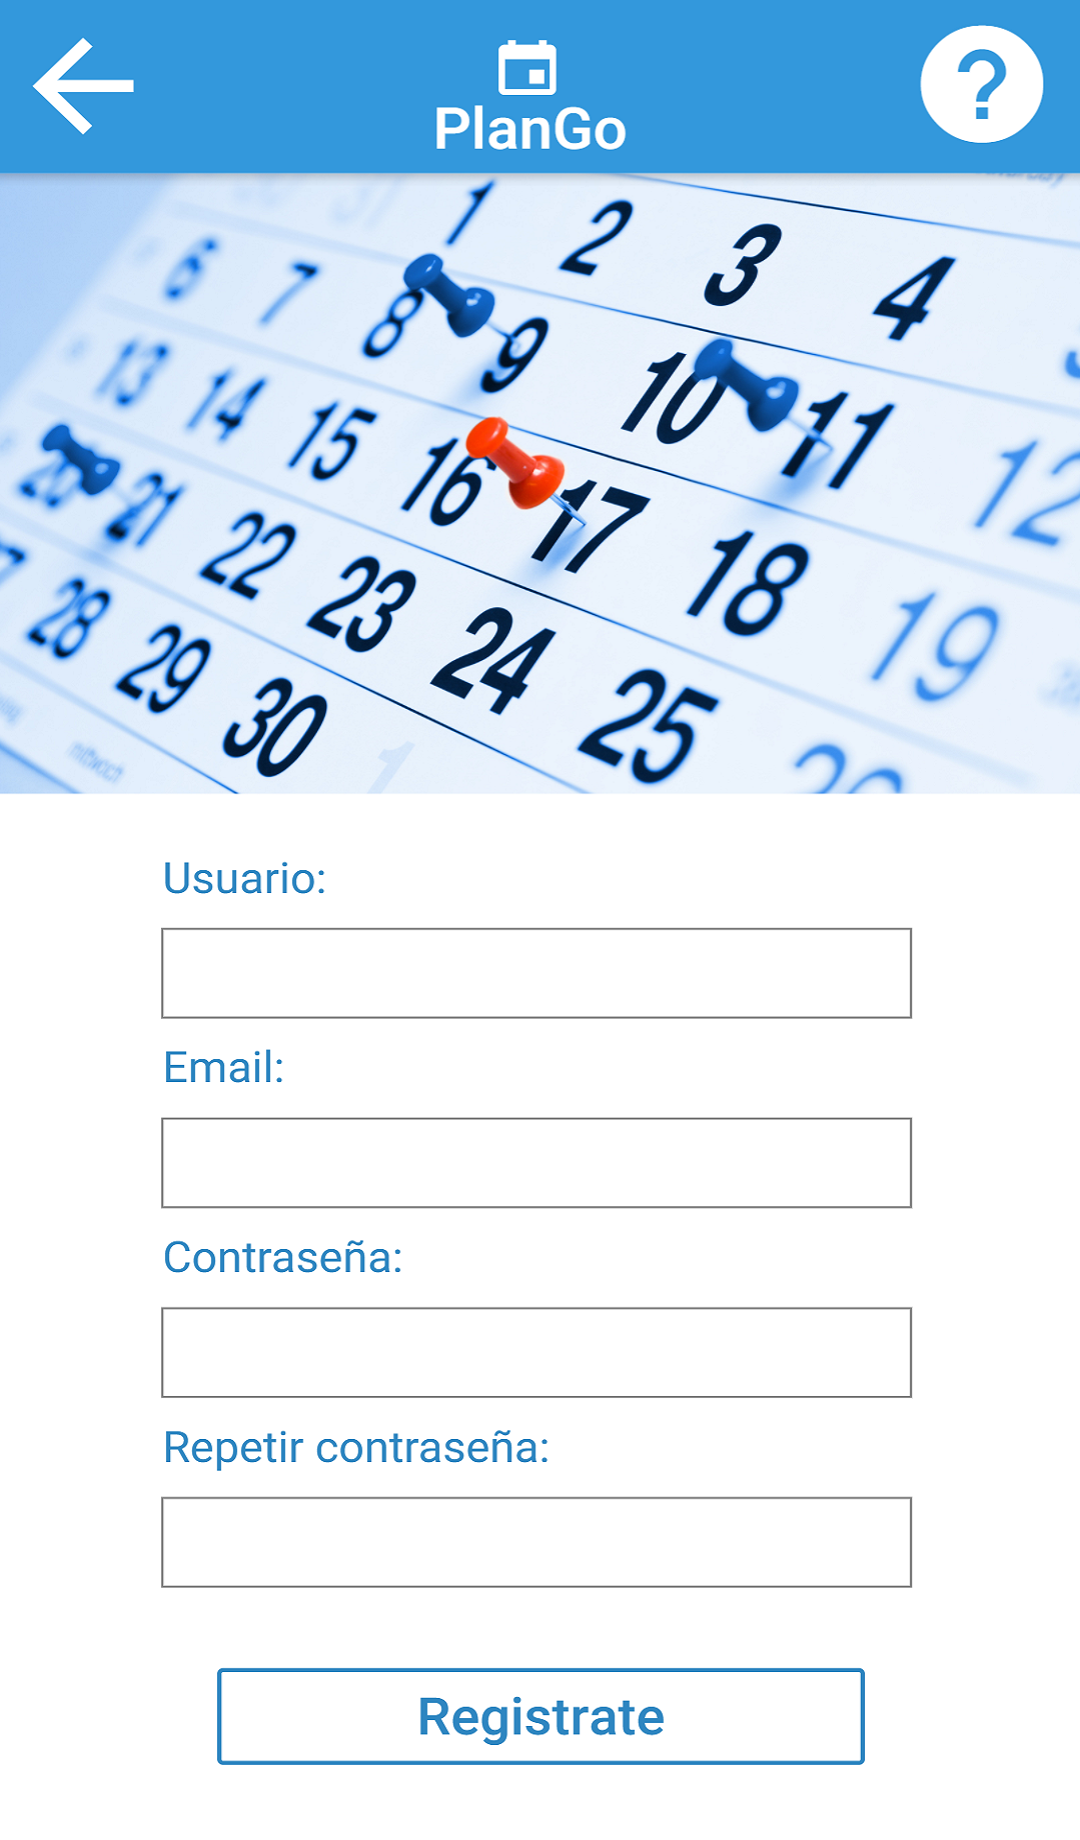
\includegraphics[width=0.3\textwidth]{img/register.png}
  \caption{Pantalla de Registro}
  \label{figura:register}
\end{figure}

\begin{figure}[H]
 \centering
  \subfloat[Nombre]{
   \label{f:error_name}
    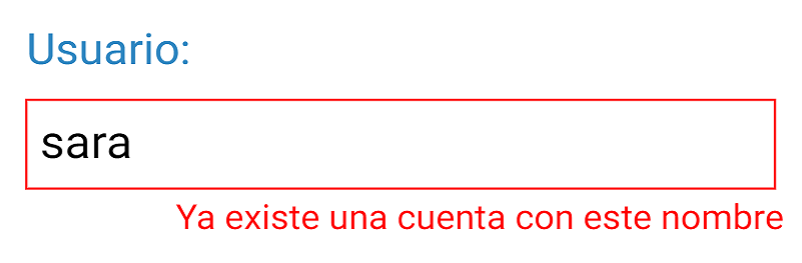
\includegraphics[width=0.3\textwidth]{img/error_name.png}}
  \subfloat[Email]{
   \label{f:error_email}
    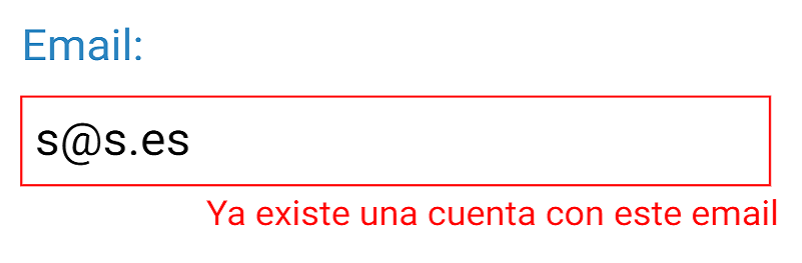
\includegraphics[width=0.3\textwidth]{img/error_email.png}}\\
  \subfloat[Contrase\~na]{
   \label{f:error_pass}
    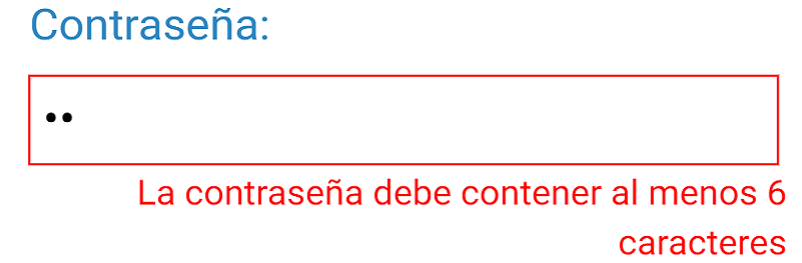
\includegraphics[width=0.3\textwidth]{img/error_pass.png}}
  \subfloat[Contrase\~na no coincide]{
   \label{f:error_pass}
    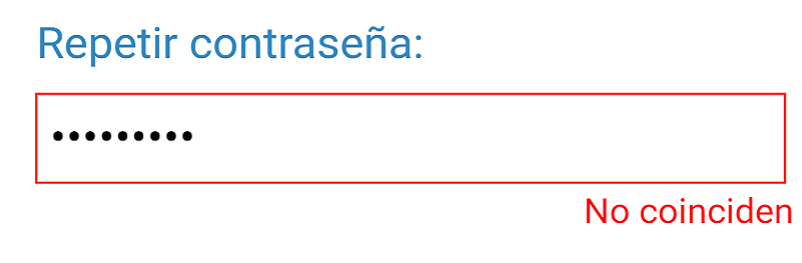
\includegraphics[width=0.3\textwidth]{img/error_pass2.png}}
 \caption{Errores pantalla de Registro}
 \label{f:animales}
\end{figure}

Contiene un formulario para los datos personales del usuario. Es un formulario reactivo
con sus correspondientes validaciones. Estas no se comprueban hasta que no se pulsa el bot\'on
'Registrate'.

\begin{itemize}
\item Usuario: mediante una petici\'on al servidor, se comprueba que no hay ning\'un usuario con
este nombre.
\item Email: se comprueba que sea un formato v\'alido y, adem\'as, mediante una petici\'on al
servidor, que no est\'e ya registrado.
\item Contrase\~na: se comprueba que no contenga menos de 6 caracteres.

\end{itemize}

He considerado que para este tipo de aplicaci\'on no son necesarios m\'as datos sobre el
usuario, lo m\'as importante es identificar quien esta votando y a quien va dirigida la encuesta.

\subsubsection{Home}
\label{sec:home}

\begin{figure}[H]
  \centering
  
\includegraphics[width=0.3\textwidth]{img/home.png}
  \caption{Pantalla de Home}
  \label{figura:home}
\end{figure}

En esta pantalla se encuentran accesos directos a distintas partes de la aplicaci\'on. Desde esta se puede acceder a todas las partes de la aplicaci\'on,
excepto al perfil que se accede mediante el men\'u lateral. 

El usuario puede acceder a sus encuestas creadas, a crear una nueva encuesta, consultar y a\~nadir a sus
amigos y acceder a las votaciones.

Al pulsar alguno de los accesos directos, se produce la navegaci\'on a la pantalla que corresponde.


\subsubsection{Header}
\label{sec:header}

\begin{figure}[H]
 \centering
  \subfloat[Men\'u]{
   \label{f:menu1}
    
\includegraphics[width=0.3\textwidth]{img/header_menu.png}}
  \subfloat[Atr\'as]{
   \label{f:atras1}
    
\includegraphics[width=0.3\textwidth]{img/header_atras.png}}
 \caption{Header}
 \label{f:header}
\end{figure}

\begin{figure}[H]
 \centering
  \subfloat[Men\'u]{
   \label{f:menu}
    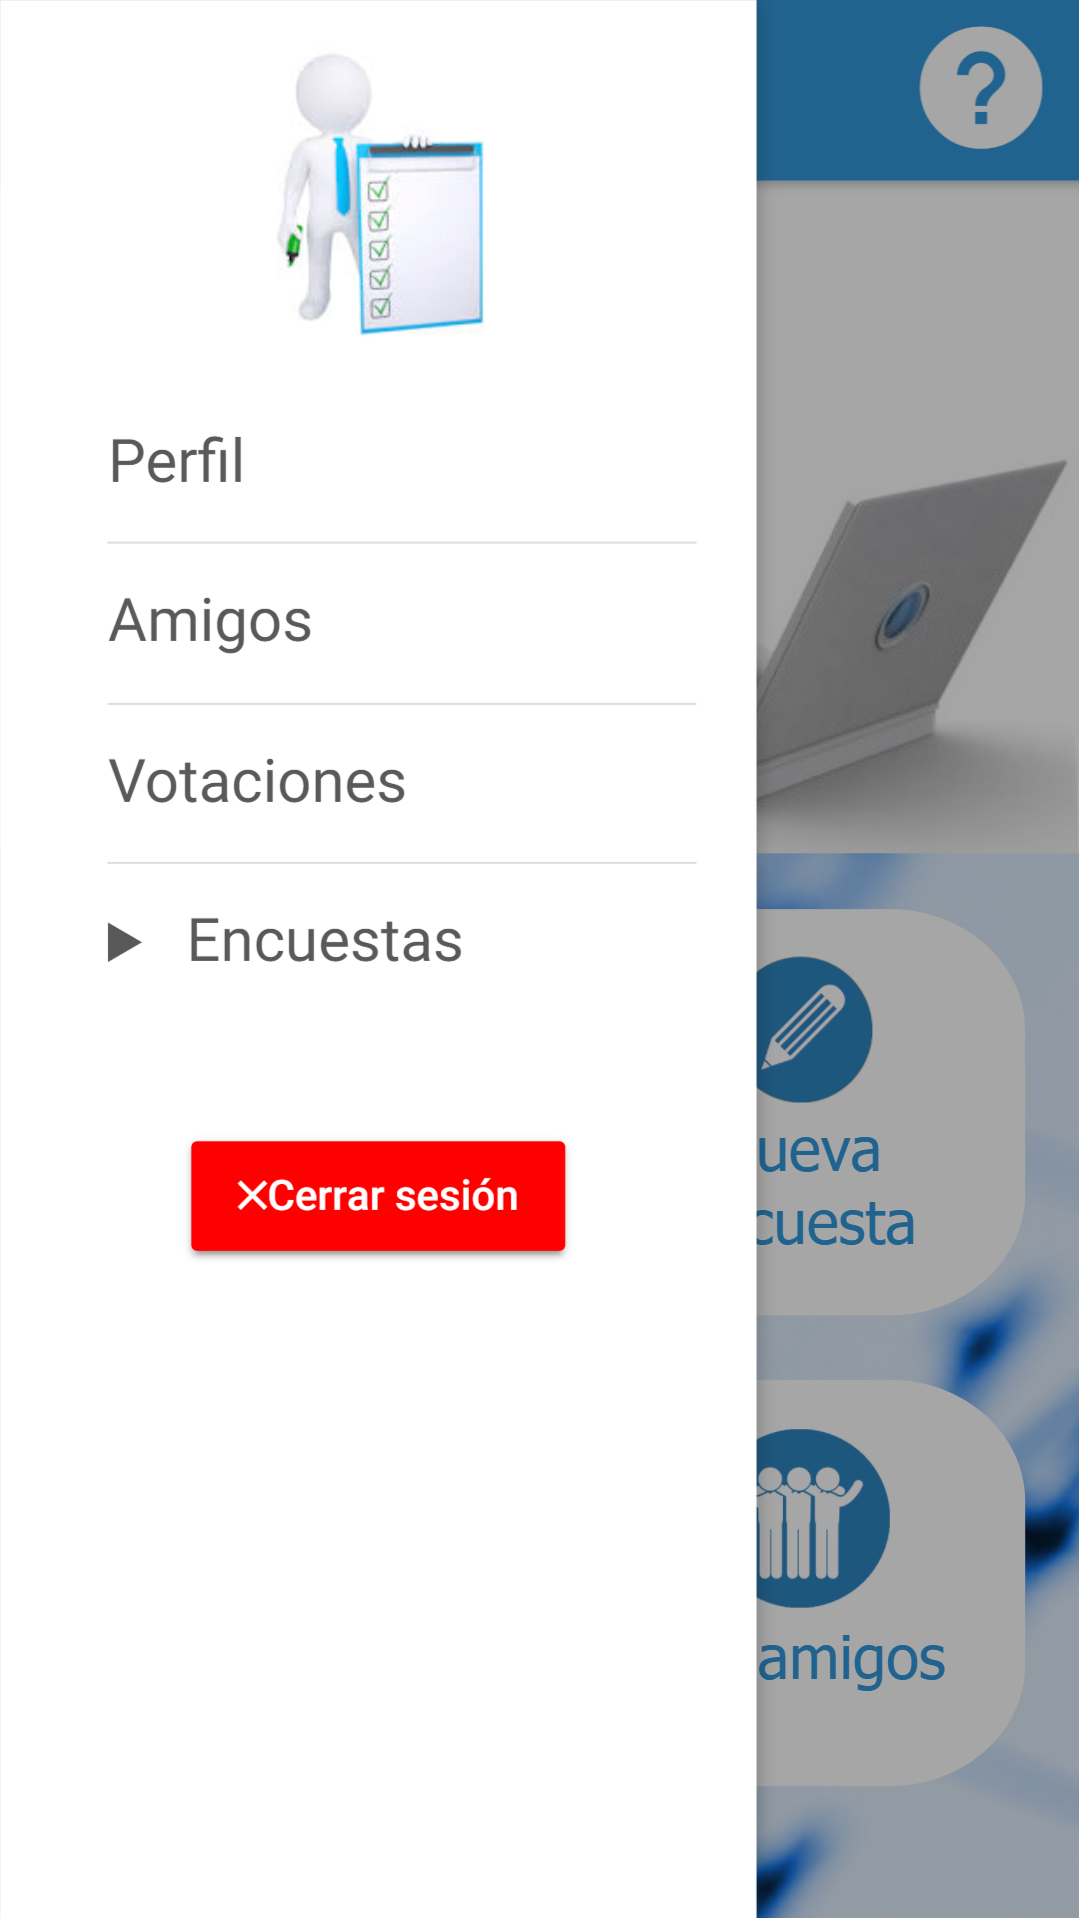
\includegraphics[width=0.3\textwidth]{img/menu.png}}
  \subfloat[Ayuda]{
   \label{f:help}
    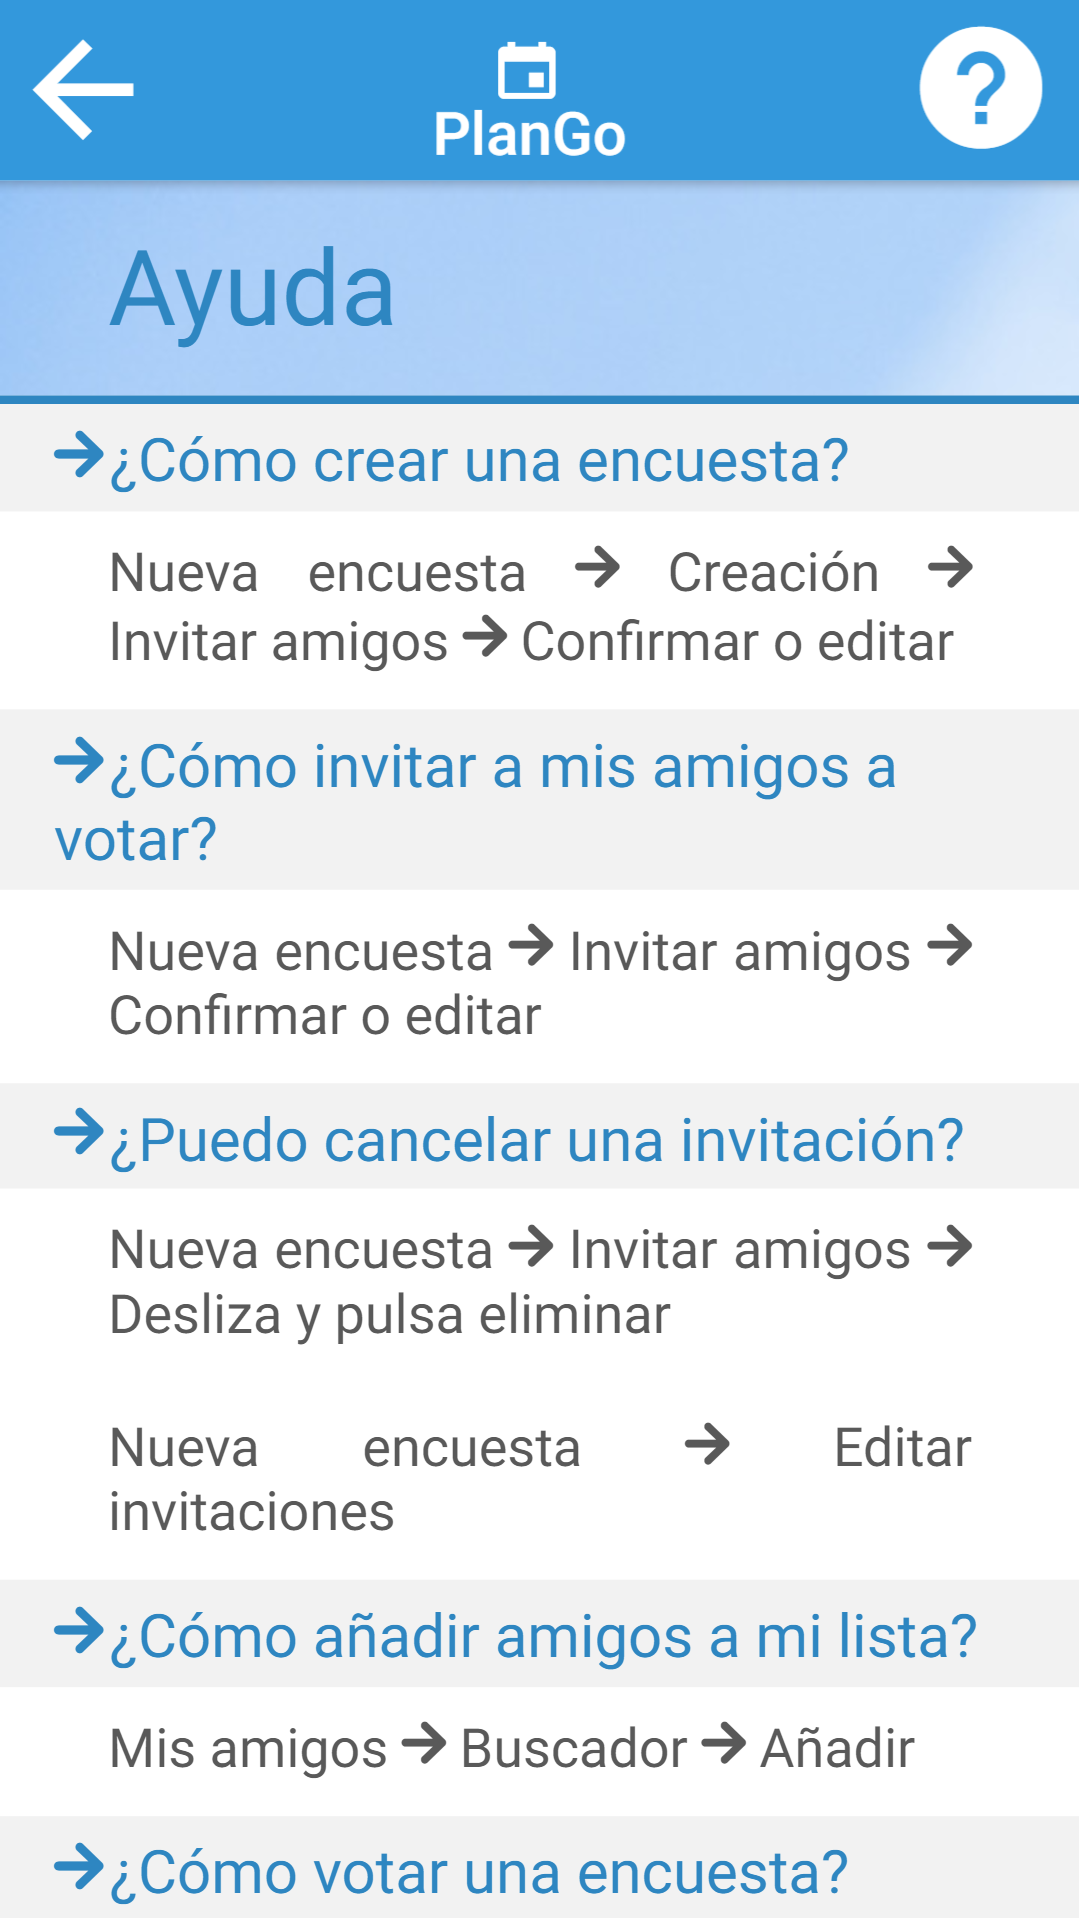
\includegraphics[width=0.3\textwidth]{img/help.png}}
 \caption{Pantalla de Men\'u y Ayuda}
 \label{f:header}
\end{figure}


El header cuenta con 4 botones:

\begin{itemize}
\item Men\'u lateral: nos permite acceder a cualquier parte de la aplicaci\'on, figura \ref{f:menu}.

\item Icono planGO: este icono te dirige a la pantalla de Home.
\item Icono ayuda: este icono te dirige a la pantalla de Ayuda, figura \ref{f:help}
\item Icono flecha: este icono te permite acceder a la pantalla anterior.
\end{itemize}

Como vemos en las figuras \ref{f:menu1} y \ref{f:atras1} el menu lateral y el icono flecha no se muestran a la vez.
Esto va a depender de la pantalla en la que nos encontremos. Cuando se produce navegaci\'on
jer\'arquica, aparece el icono atr\'as, para el resto de los casos aparece el icono de men\'u.



\subsubsection{Mis encuestas}
\label{sec:mis_encuestas}

\begin{figure}[H]
 \centering
  \subfloat[Listado]{
   \label{f:polls}
   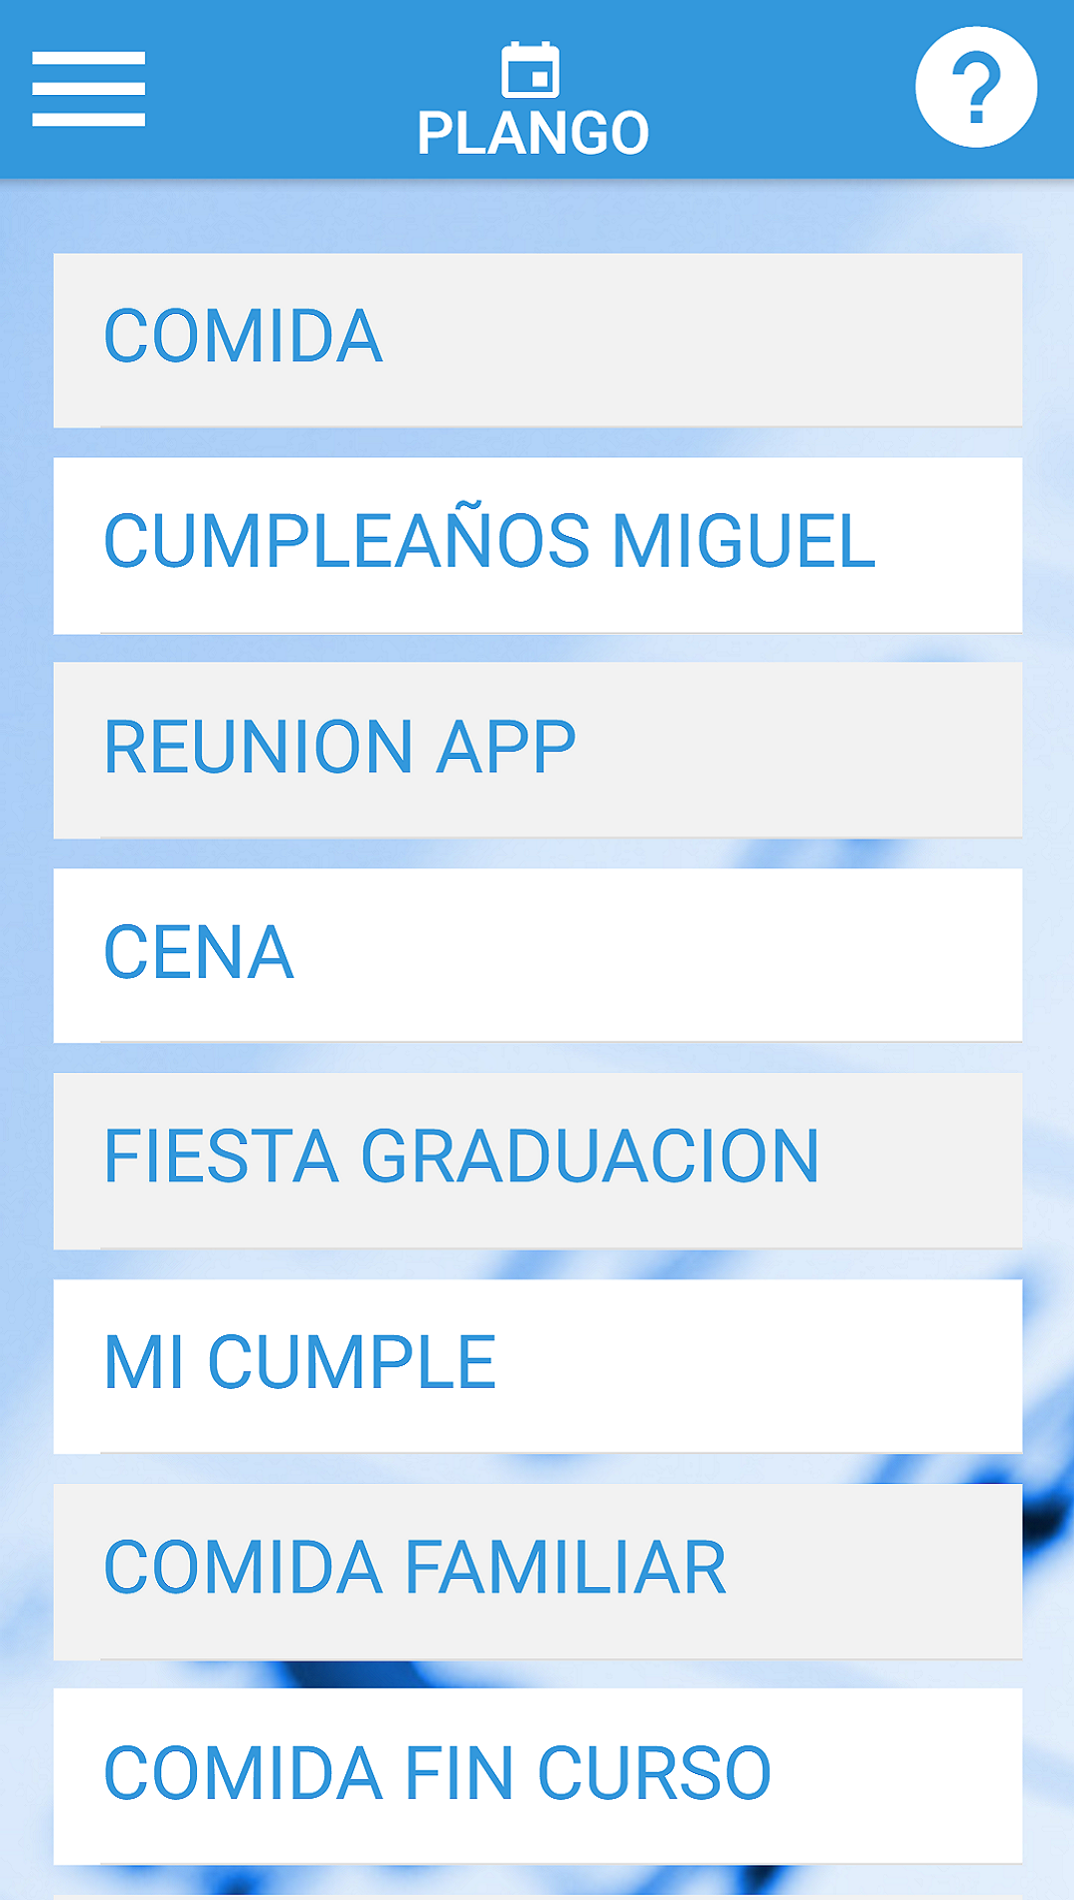
\includegraphics[width=0.3\textwidth]{img/mis_encuestas.png}}
  \subfloat[Detalle]{
   \label{f:scroll_tabla}
    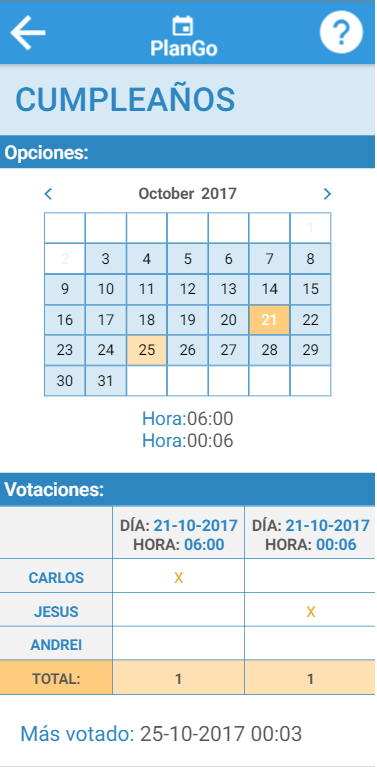
\includegraphics[width=0.3\textwidth]{img/votos_1.png}}
  \caption{Pantalla de Mis encuestas}
 \label{f:mis_encuestas}
\end{figure}

En esta pantalla el usuasio tiene acceso a todas las encuestas que han sido creadas por \'el.
Como vemos en la figura \ref{f:polls}, aparece un listado con todas las encuestas. Es posible hacer click en
cualquiera de las encuestas para acceder a los votos que ha obtenido.

Si no hay votos para la encuesta seleccionada, se mostrara un mensaje de aviso. En caso de que haya
votaciones, la pantalla mostrada varia en funci\'on si es de tipo texto o de tipo fecha.

Cuando la encuesta es de tipo texto, se muestra una tabla con las opciones que tiene disponibles la encuesta
y un recuento de votos por usuario. Cuando la encuesta es de tipo fecha, aparece un calendario con los d\'ias
que existen como opci\'on remarcados. Estos d\'ias se pueden pulsar, para que aparezca el detalle de las horas
a elegir, en caso de que las haya. Despu\'es hay una tabla igual que la descrita anteriormente para tipo texto.

Debido a que la tabla crece horizontalmente seg\'un sea el n\'umero de opciones, esta tabla permite realizar \emph{scroll} horizontal. 




\subsubsection{Mis amigos}
\label{sec:mis_amigos}

\begin{figure}[H]
 \centering
  \subfloat[Listado]{
   \label{f:lista}
    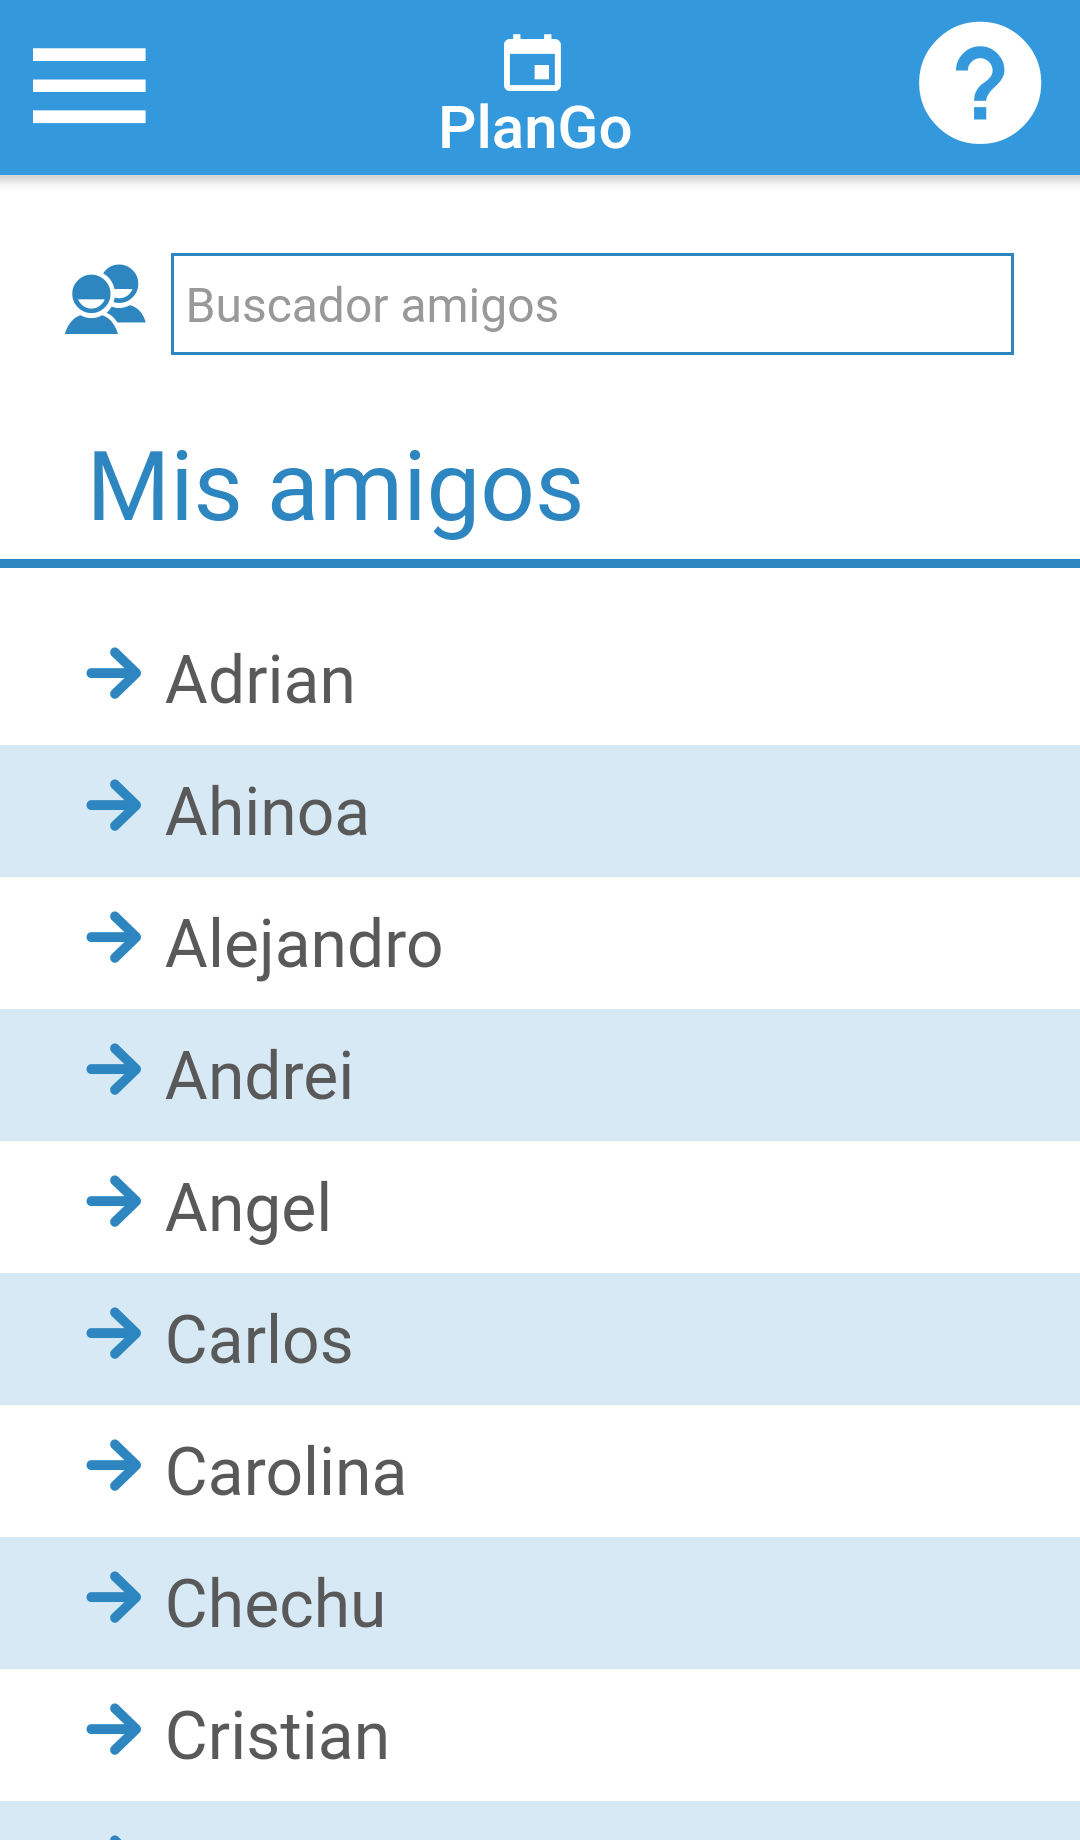
\includegraphics[width=0.3\textwidth]{img/mis_amigos.png}}
  \subfloat[Buscador]{
   \label{f:buscar}
    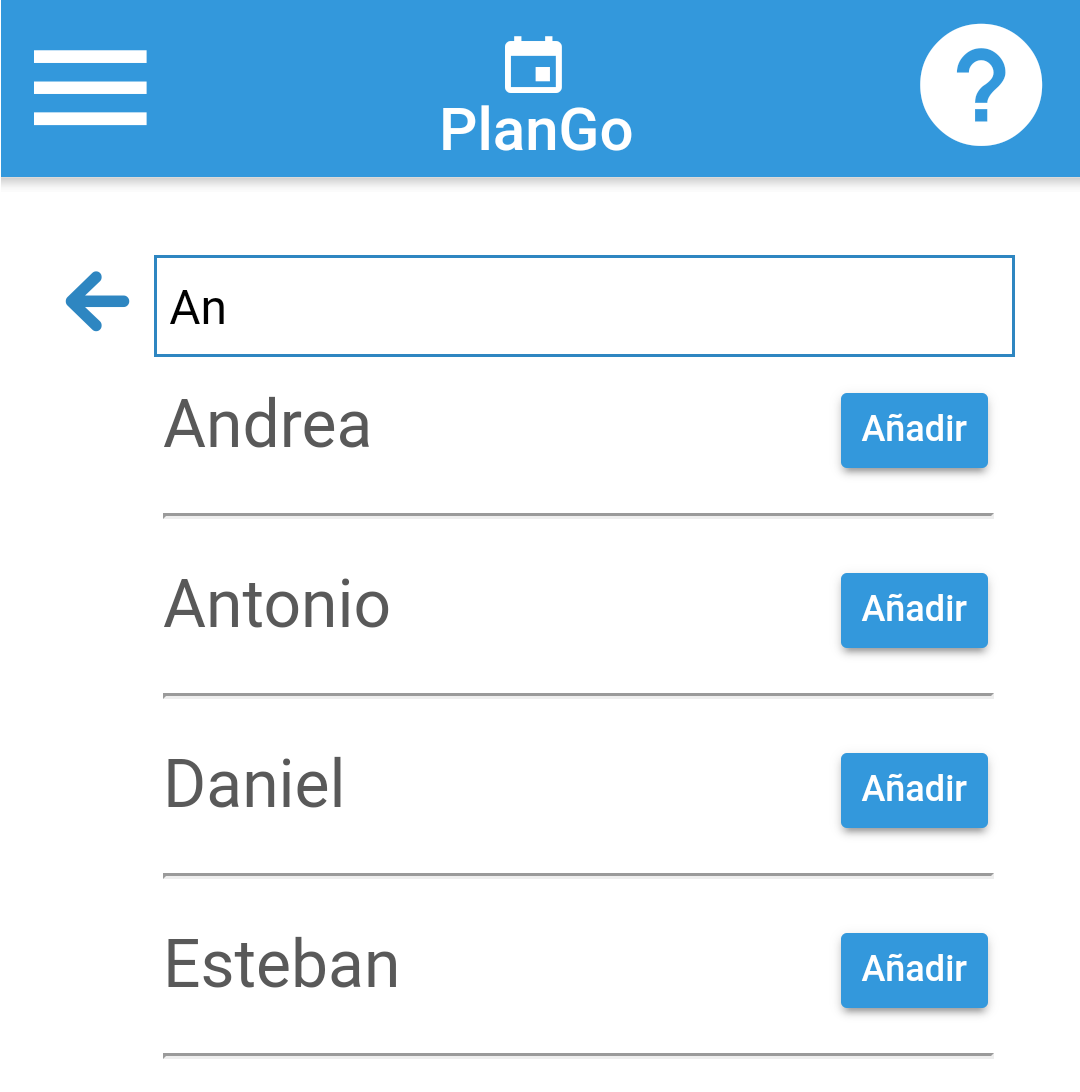
\includegraphics[width=0.3\textwidth]{img/mis_amigos_buscar.png}}
 \caption{Pantalla de Mis amigos}
 \label{f:mis_amigos}
\end{figure}

Esta pantalla contiene un buscador en la parte superior y un listado, como se puede ver en
la figura \ref{f:lista}.

El buscador permite encontrar usuarios, que tengan cuenta en la aplicaci\'on, introduciendo
su nombre. Este filtro tiene autocompletar, de tal manera que el listado de b\'usqueda se va actualizando
a la vez que el usuario va introduciendo caracteres. Esto es muy \'util para el usuario,
pues no tiene porque saber el nombre exacto del usuario que quiere buscar. Solo aparecen los
usuarios que a\'un no tiene en su lista de amigos. En el caso de querer cerrar esta b\'usqueda,
existe un bot\'on con forma de flecha, para volver al estado anterior.

Para a\~nadir un nuevo amigo, tras haber realizado su b\'usqueda, hay que pulsar en el bot\'on
'a\~nadir'.

En el listado se ven todos los usuarios que contiene en su lista de amigos.


\subsubsection{Perfil}
\label{sec:perfil}

\begin{figure}[H]
 \centering
  \subfloat[Cambio nombre]{
   \label{f:nombre}
    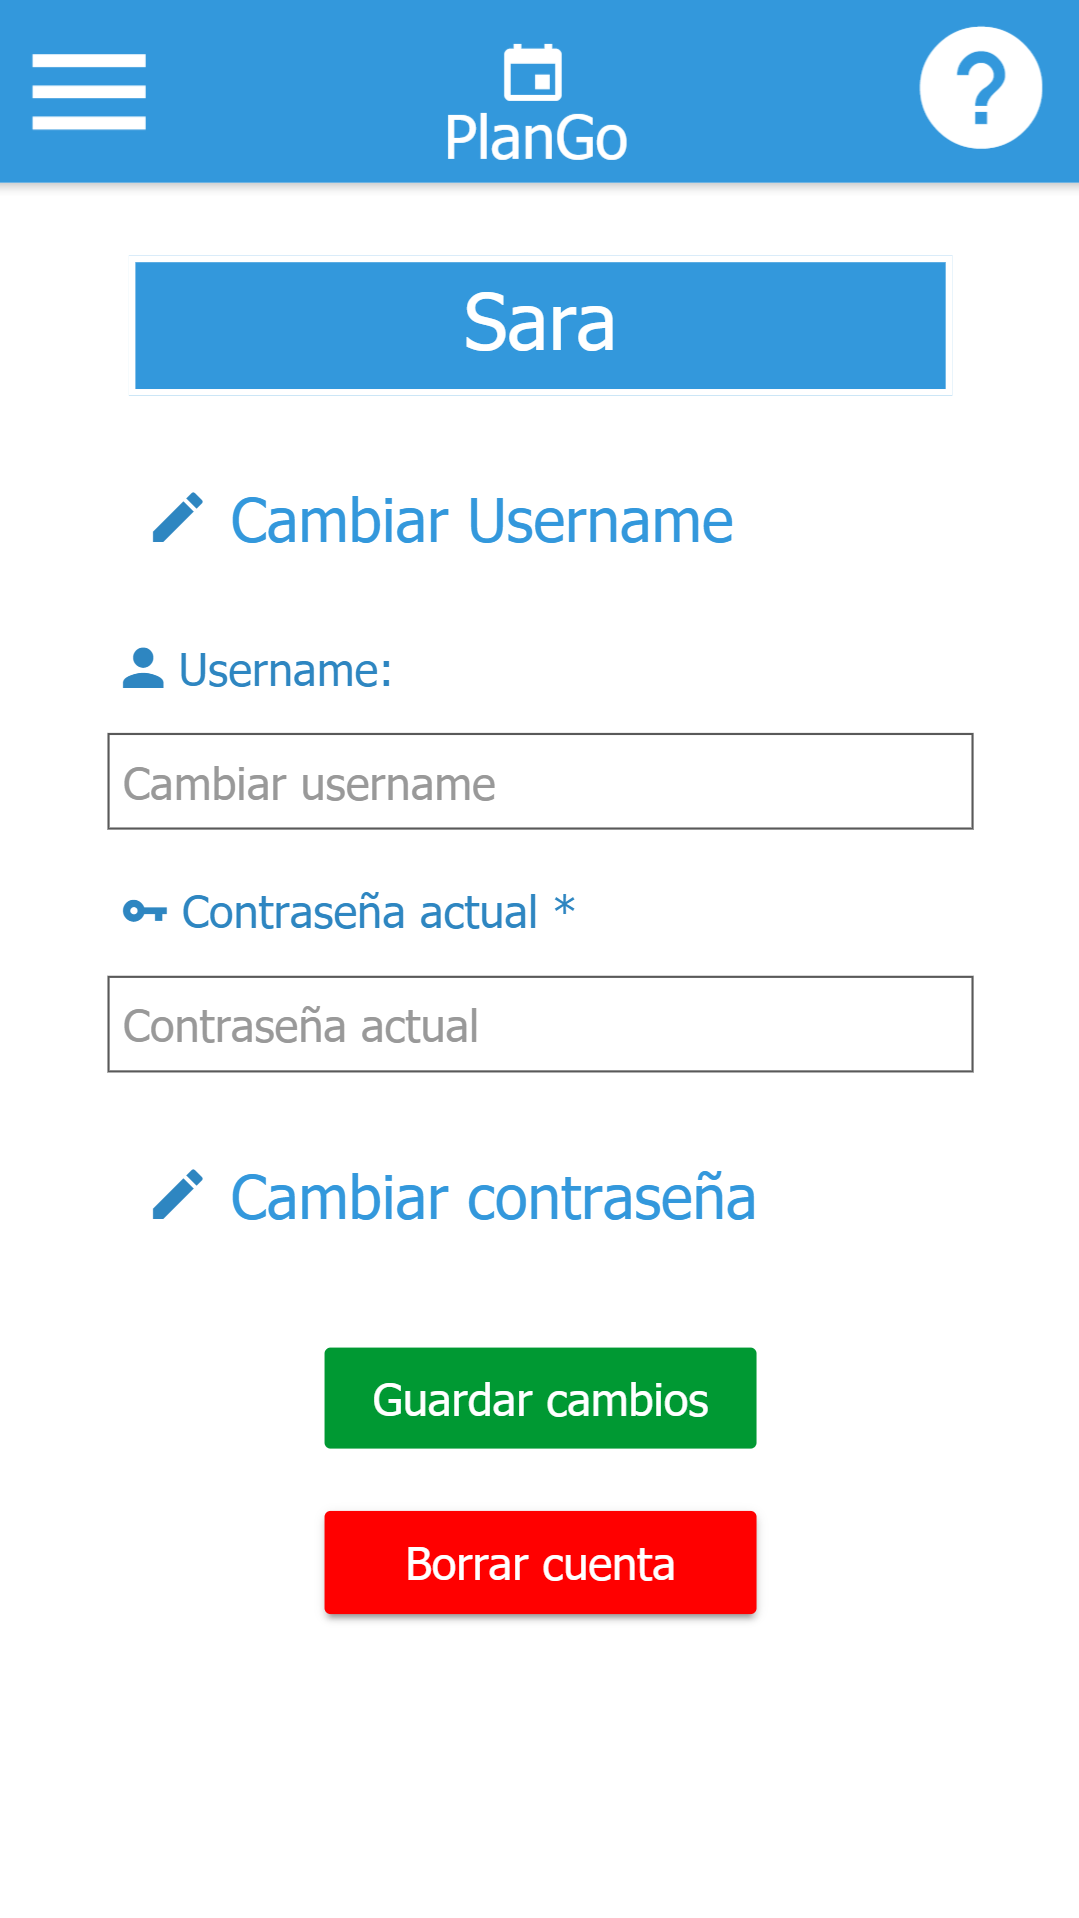
\includegraphics[width=0.3\textwidth]{img/perfil1.png}}
  \subfloat[Cambio contrase\~na]{
   \label{f:contrasena}
    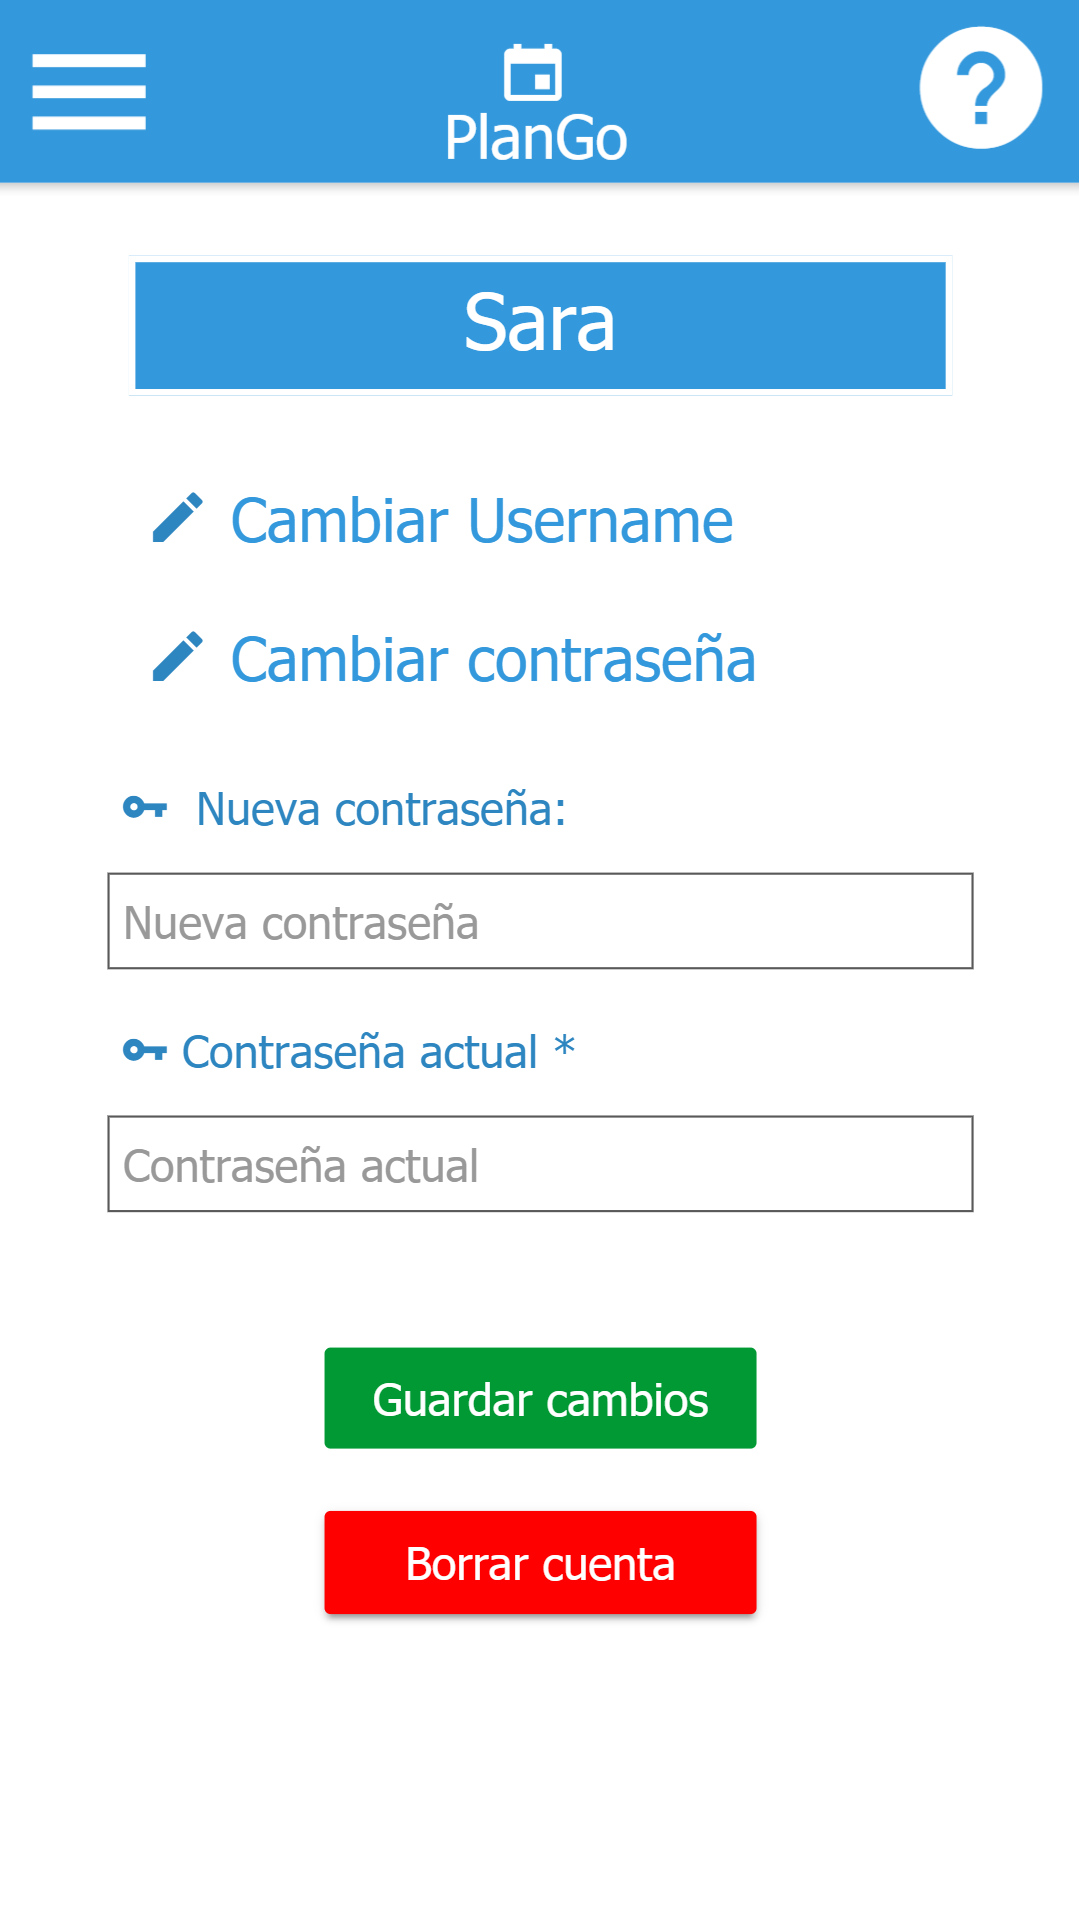
\includegraphics[width=0.3\textwidth]{img/perfil2.png}}
 \caption{Pantalla de Perfil}
 \label{f:perfil}
\end{figure}

Esta pantalla contiene dos desplegables, cada uno de los cuales esta destinado a una funci\'on
diferente. Es una pantalla bastante intuitiva como se ve en la fig.

En el desplegable 'Cambiar Username' el usuario podr\'a cambiar el nombre con el que esta
identificado en la aplicaci\'on. En el caso del desplegable 'Cambiar contrase\~na' el usuario podr\'a
cambiar su contrase\~na actual.

Para todos los cambios que se realicen en el perfil del usuario, por seguridad, es necesario
que introduzca la contrase\~na actual. De esta manera s\'olo el propio usuario conocedor de su
contrase\~na podr\'a realizar cambios.


\subsubsection{Nueva encuesta}
\label{sec:nueva_encuesta}

\begin{figure}[H]
 \centering
  \subfloat[Selecci\'on tipo]{
   \label{figura:tipo_encuestas}
    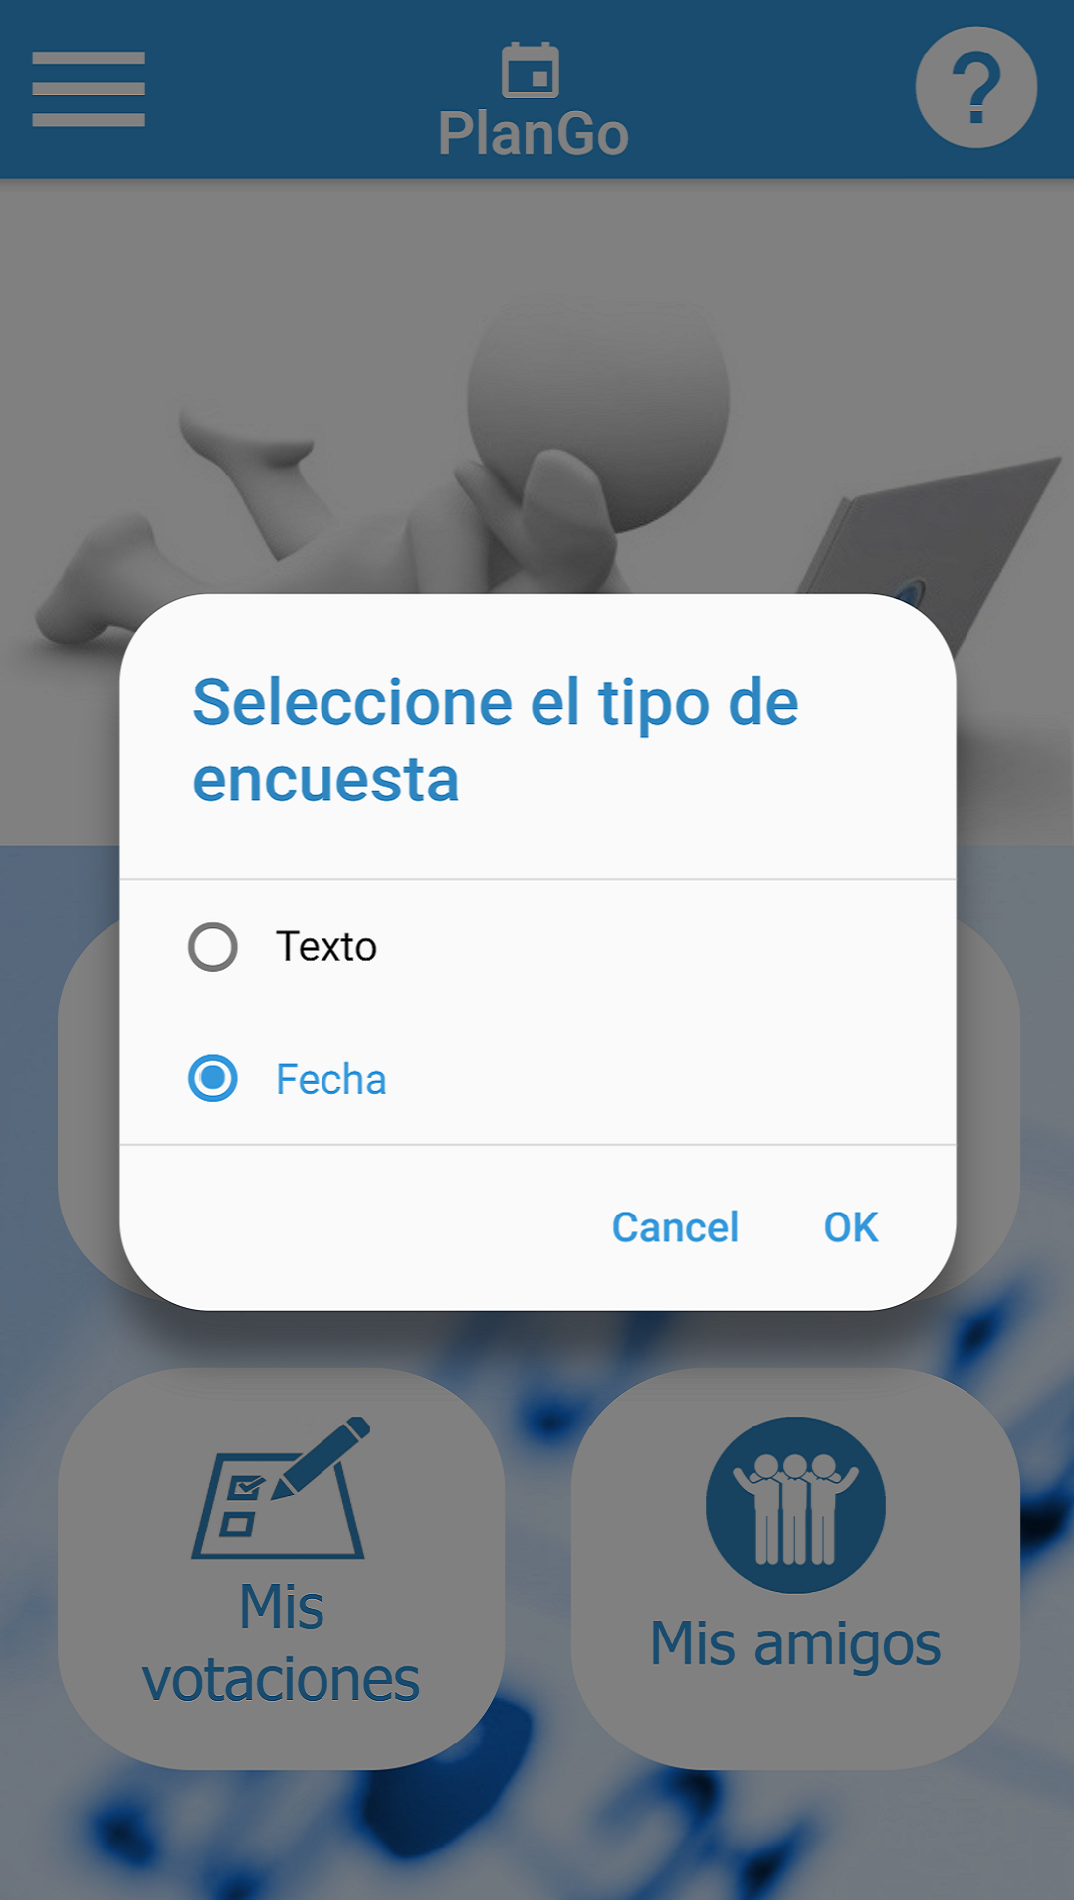
\includegraphics[width=0.3\textwidth]{img/t_fecha.png}}
  \subfloat[Tipo texto]{
   \label{f:t_texto}
    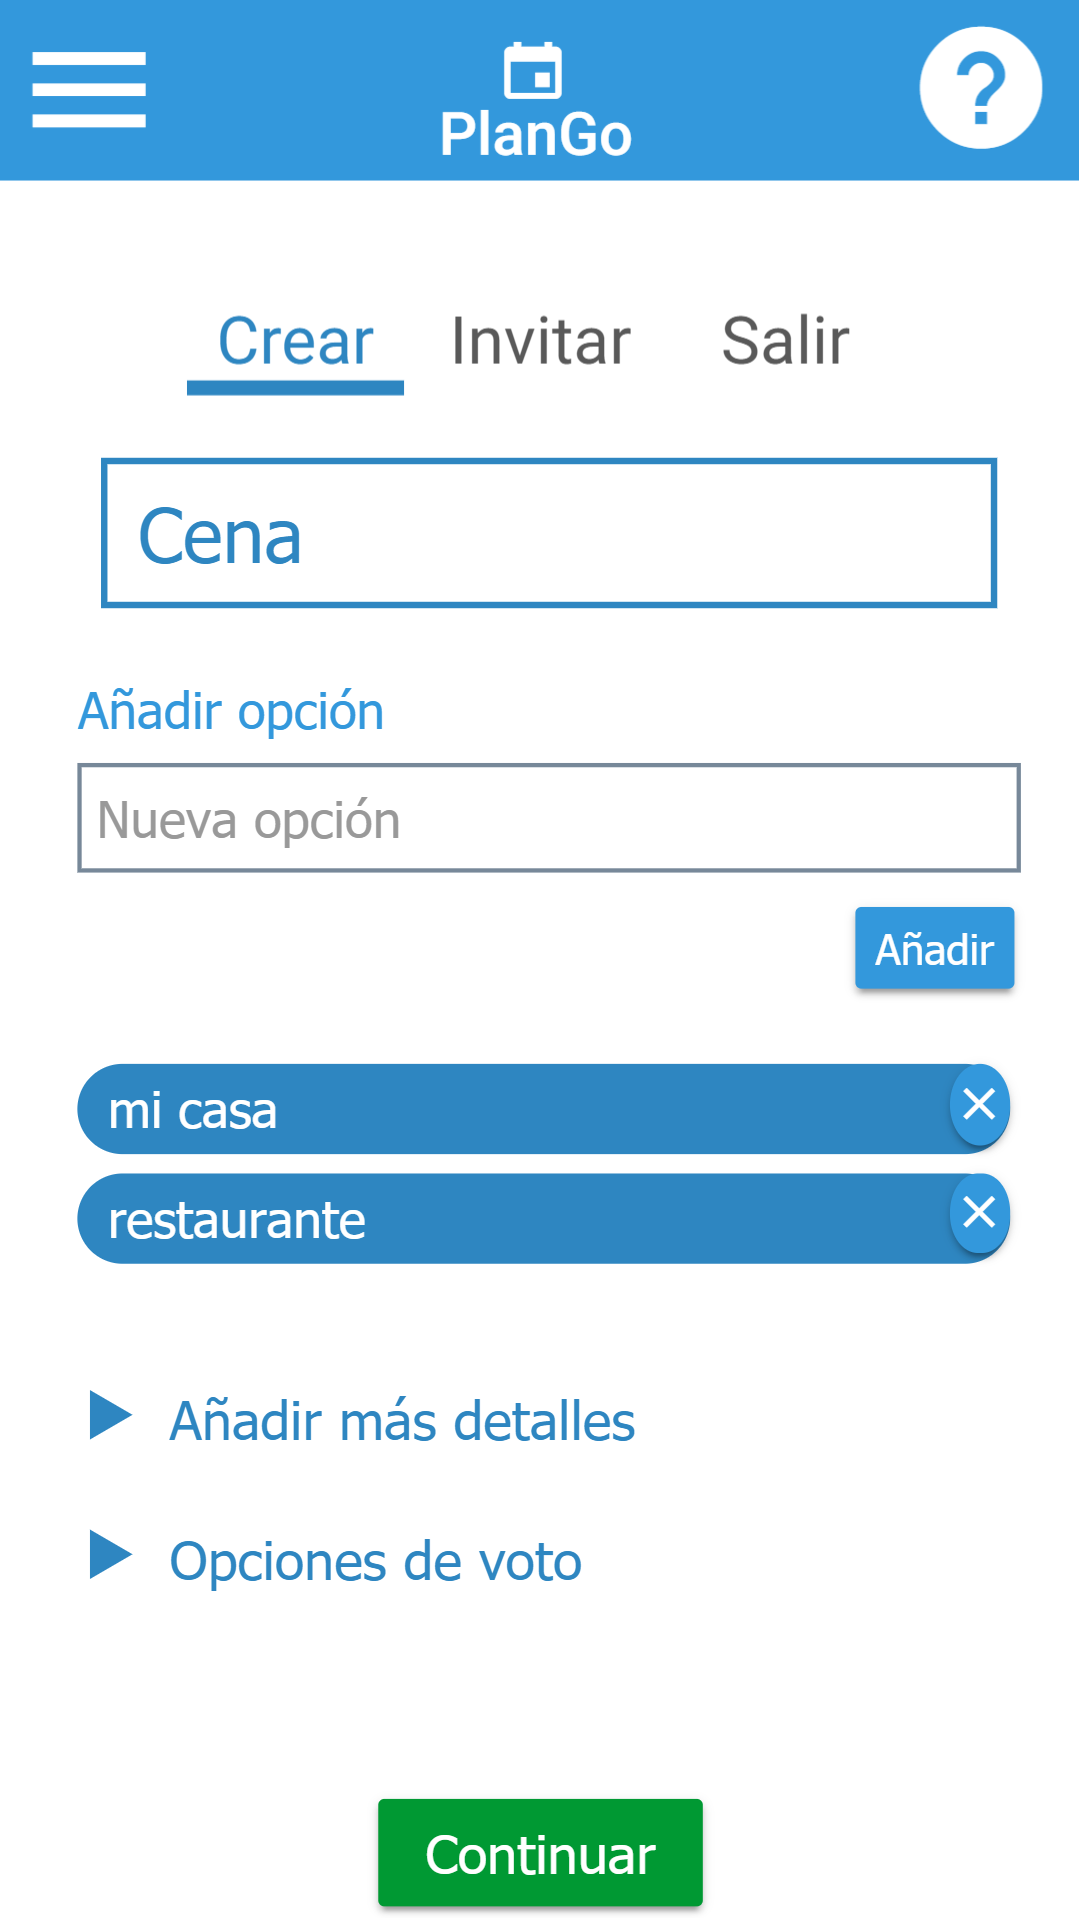
\includegraphics[width=0.3\textwidth]{img/texto.png}}
  \subfloat[Tipo fecha]{
   \label{f:fecha}
    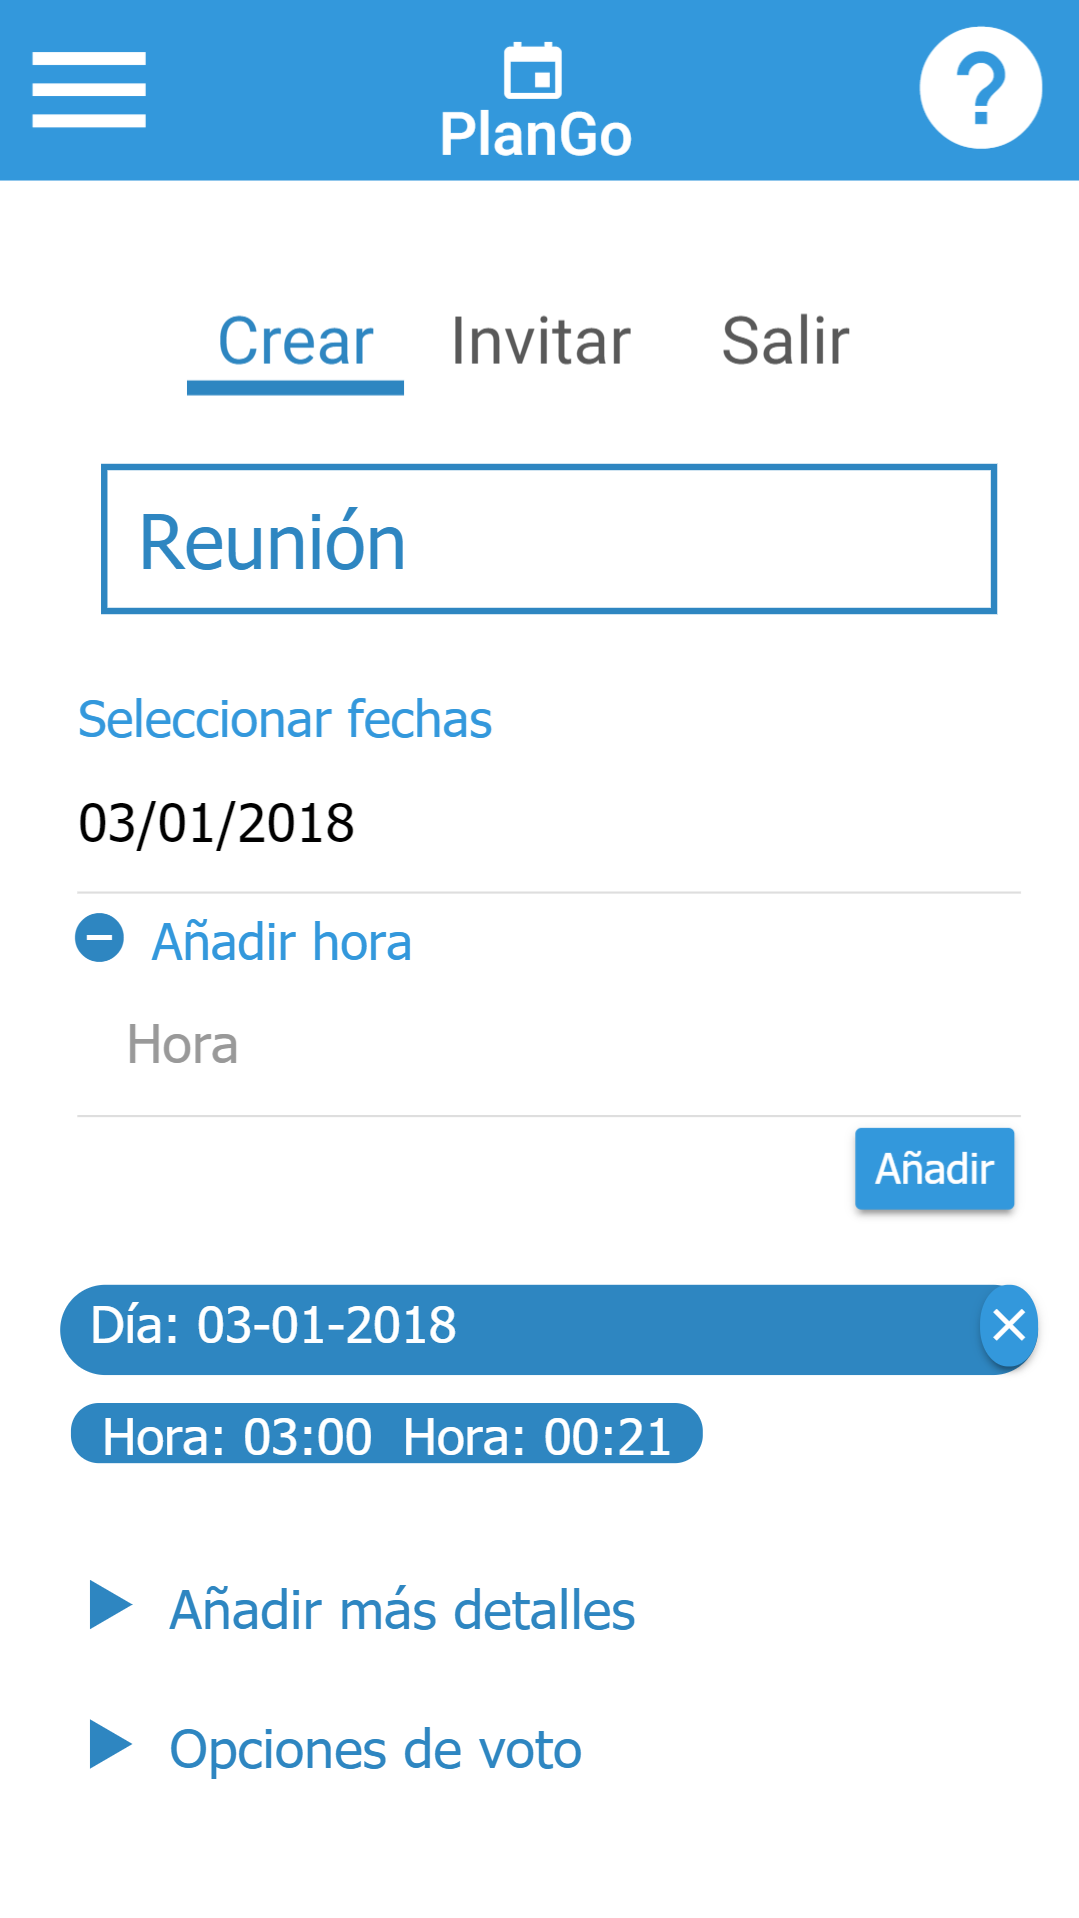
\includegraphics[width=0.3\textwidth]{img/fecha.png}}
 \caption{Pantalla de Nueva encuesta: paso 1}
 \label{f:poll}
\end{figure}

\begin{figure}[H]
 \centering
  \subfloat[Listado]{
   \label{f:nueva2}
    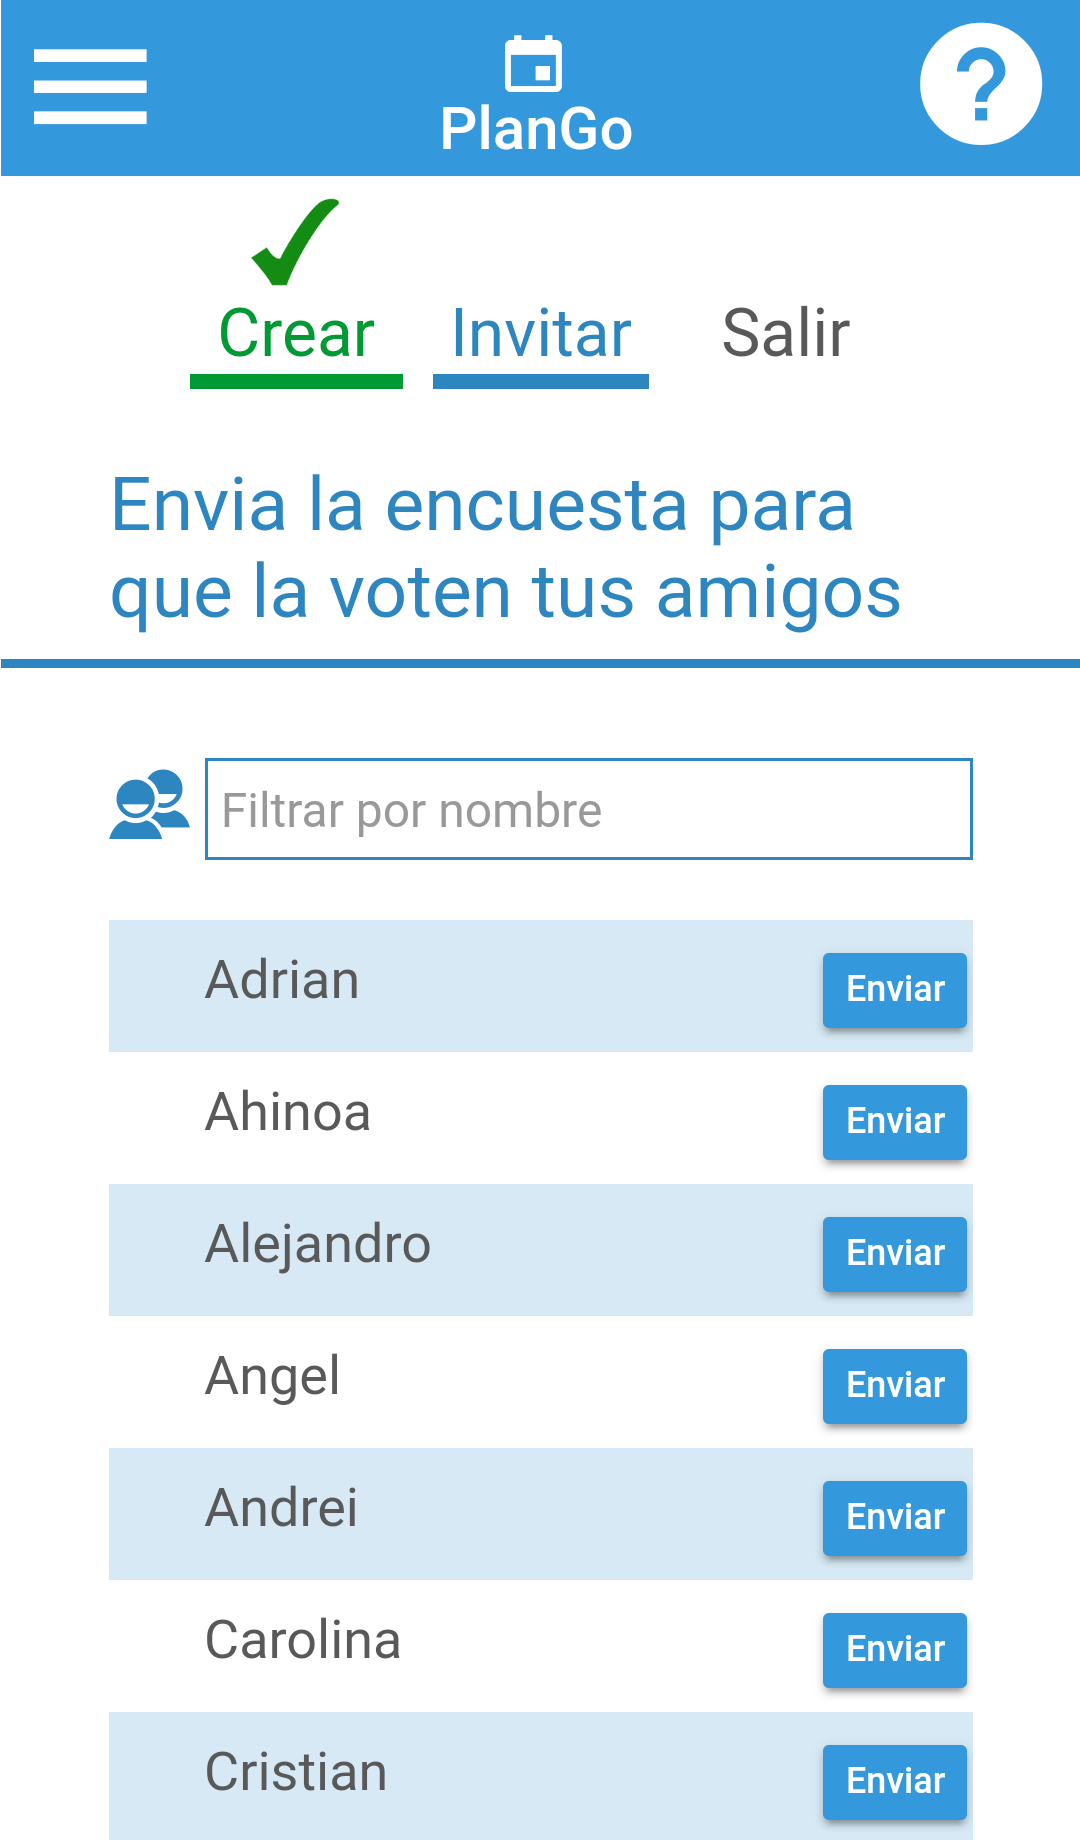
\includegraphics[width=0.3\textwidth]{img/nueva_2.png}}
  \subfloat[Invitaciones]{
   \label{f:nueva21}
    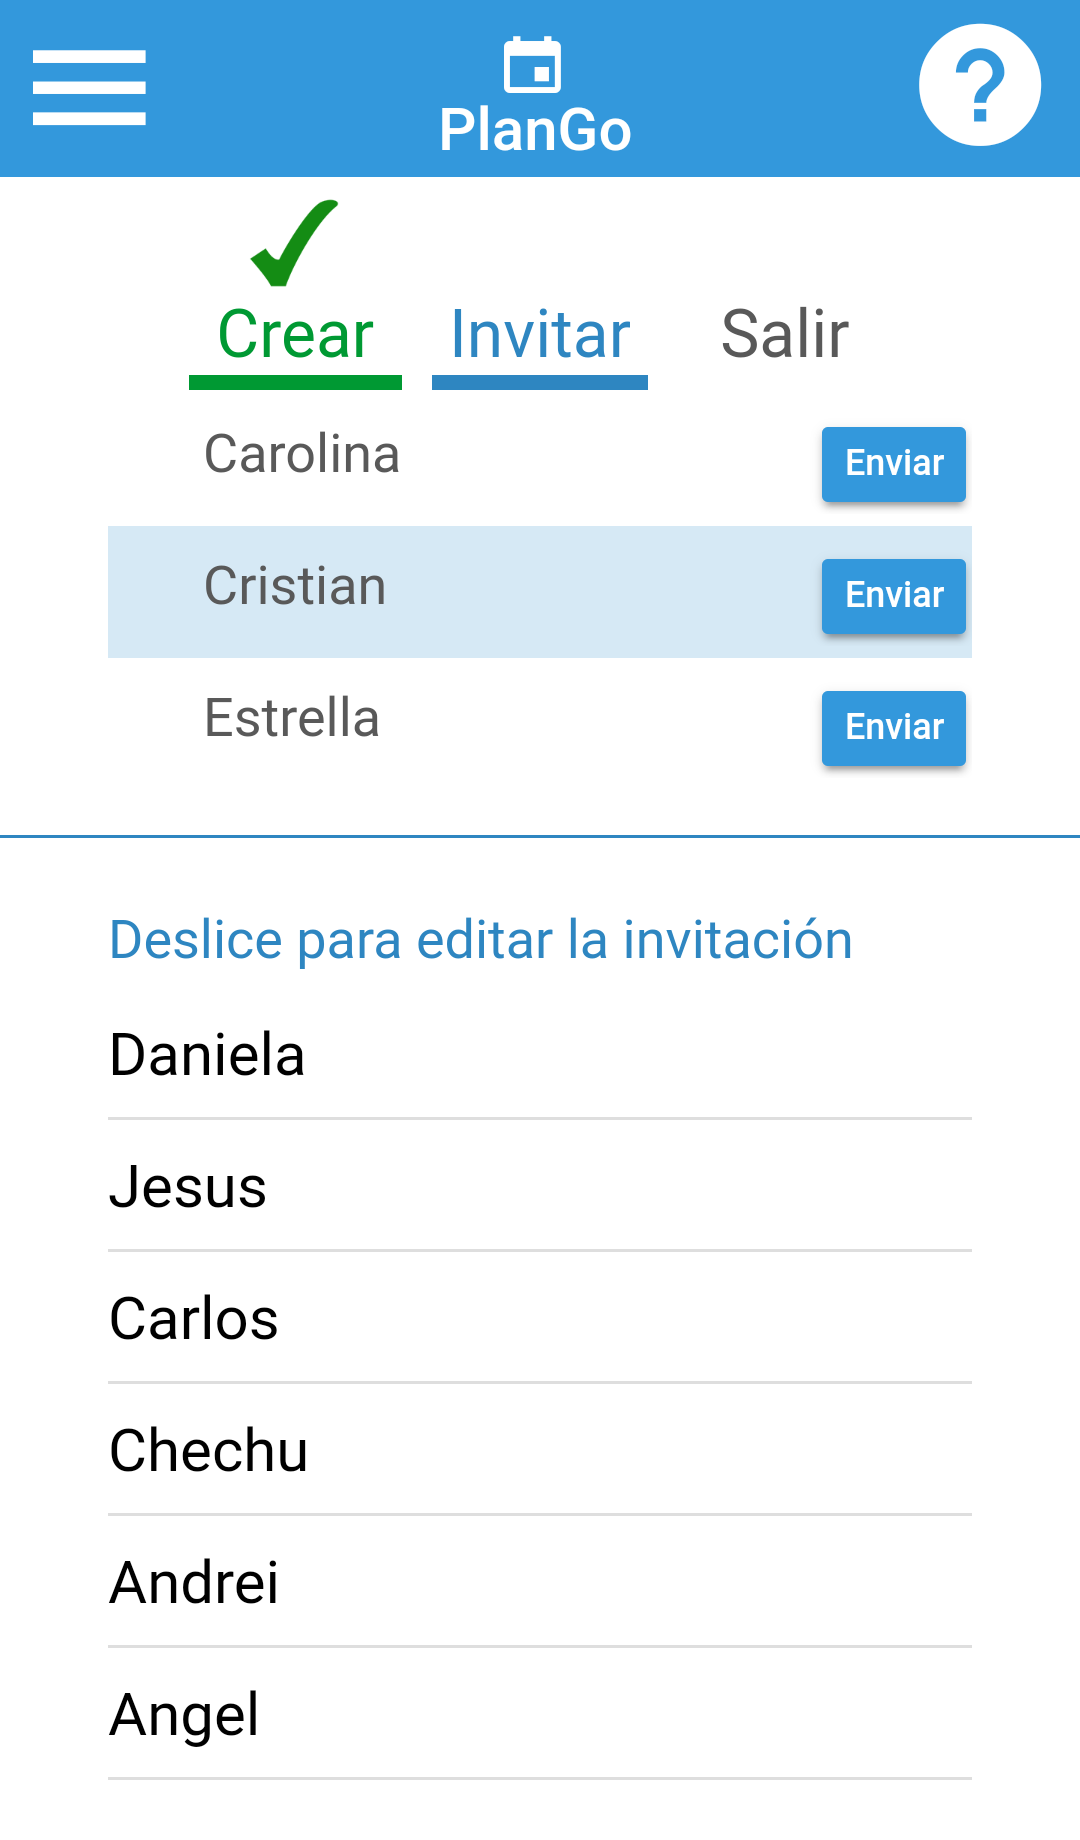
\includegraphics[width=0.3\textwidth]{img/nueva_21.png}}
\subfloat[Eliminar]{
   \label{f:nueva22}
    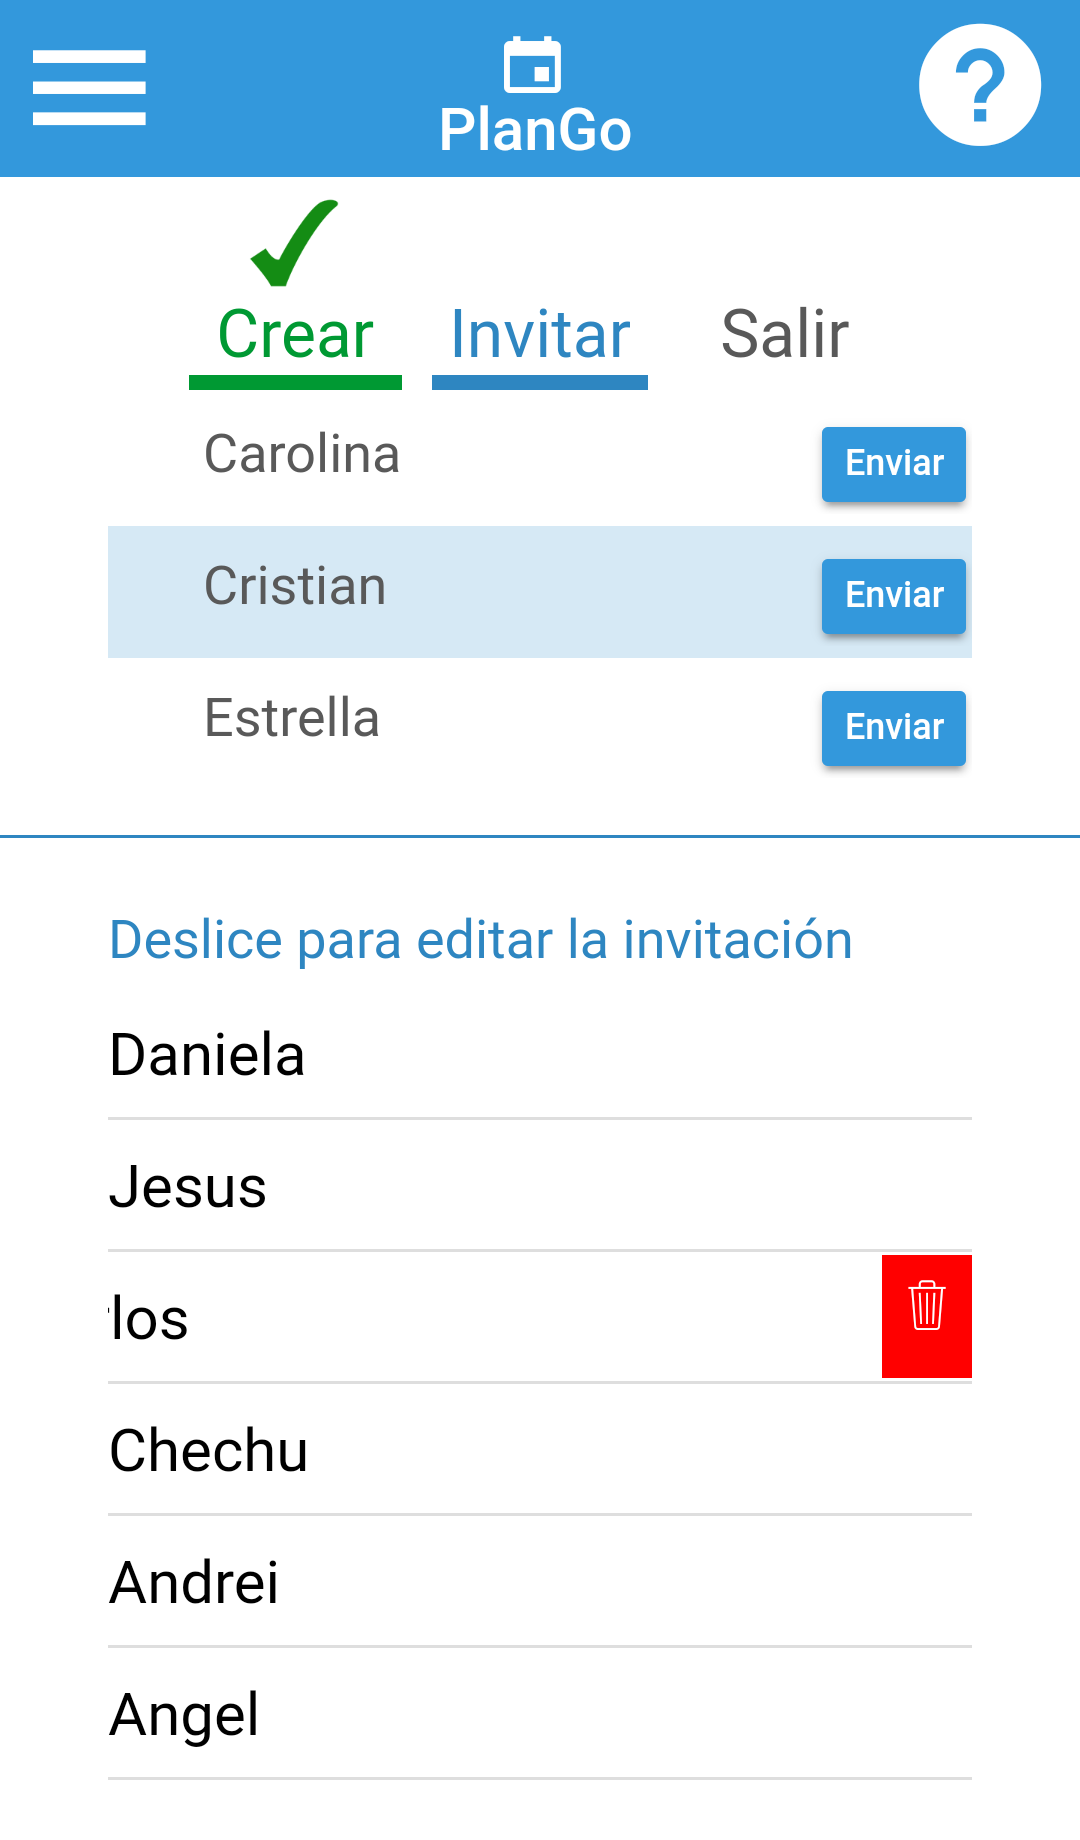
\includegraphics[width=0.3\textwidth]{img/nueva_22.png}}
 \caption{Pantalla de Nueva encuesta: paso 2}
 \label{f:enviar_encuesta}
\end{figure}


Esta es la parte principal de la aplicaci\'on, la creaci\'on de la encuesta.
Existen dos tipos de encuesta: por fecha o por texto. En una encuesta por fecha, se podr\'a 
votar sobre fechas y horas. En el caso de una encuesta por texto las votaciones se realizar\'an
entre textos que pueden ser de cualquier tipo. Como se ve en la figura \ref{figura:tipo_encuestas}, esta elecci\'on se hace
en una alerta que aparece al pulsar el bot\'on 'Nueva encuesta'.

Una vez selecionado el tipo de encuesta que se quiere crear, se accede a rellenar los datos
necesarios para la encuesta, como se ve en la figura \ref{f:poll}. El formulario contiene varios campos, los
cuales algunos son opcionales y otros no.

Los campos requeridos son el t\'itulo y las opciones,
si esto no se cumple, se mostrar\'a el campo erroneo en rojo. Dentro de los campos opcionales 
encontramos que se puede a\~nadir una ubicaci\'on o un comentario. Adem\'as de esto, hay una opci\'on
que restringe la encuesta a un solo voto por votante.

Una vez completado el primer paso, pasamos al segundo. En este, el usuario tiene que elegir 
a que amigos enviar la encuesta. De esta manera, estos podr\'an realizar su voto. 

Como se ve en la figura \ref{f:enviar_encuesta}, en este paso encontramos un buscador y un listado. El buscador tiene la funcionalidad de facilitar al usuario
la b\'usqueda de aquellos amigos a los que quiere enviar la encuesta. En el listado aparecen todos los amigos
con un bot\'on de 'Enviar'. Este bot\'on envia la encuesta al usuario seleccionado. En la figura \ref{f:nueva21} 
se puede ver el resumen que se genera de todas las invitaciones realizadas. En el caso de querer cancelar
una invitaci\'on es posible arrastrando sobre el nombre y pulsando en la papelera como se ve en la figura \ref{f:nueva22}. 

Una vez completados estos pasos, en el \'utimo paso tenemos la posibilidad de modificar datos introducidos 
durante la creaci\'on de la encuesta o modificar las invitaciones a amigos. 


\subsubsection{Votaciones pendientes}
\label{sec:votacion_pendiente}

\begin{figure}[H]
 \centering
  \subfloat[Pendientes]{
   \label{f:pendientes}
    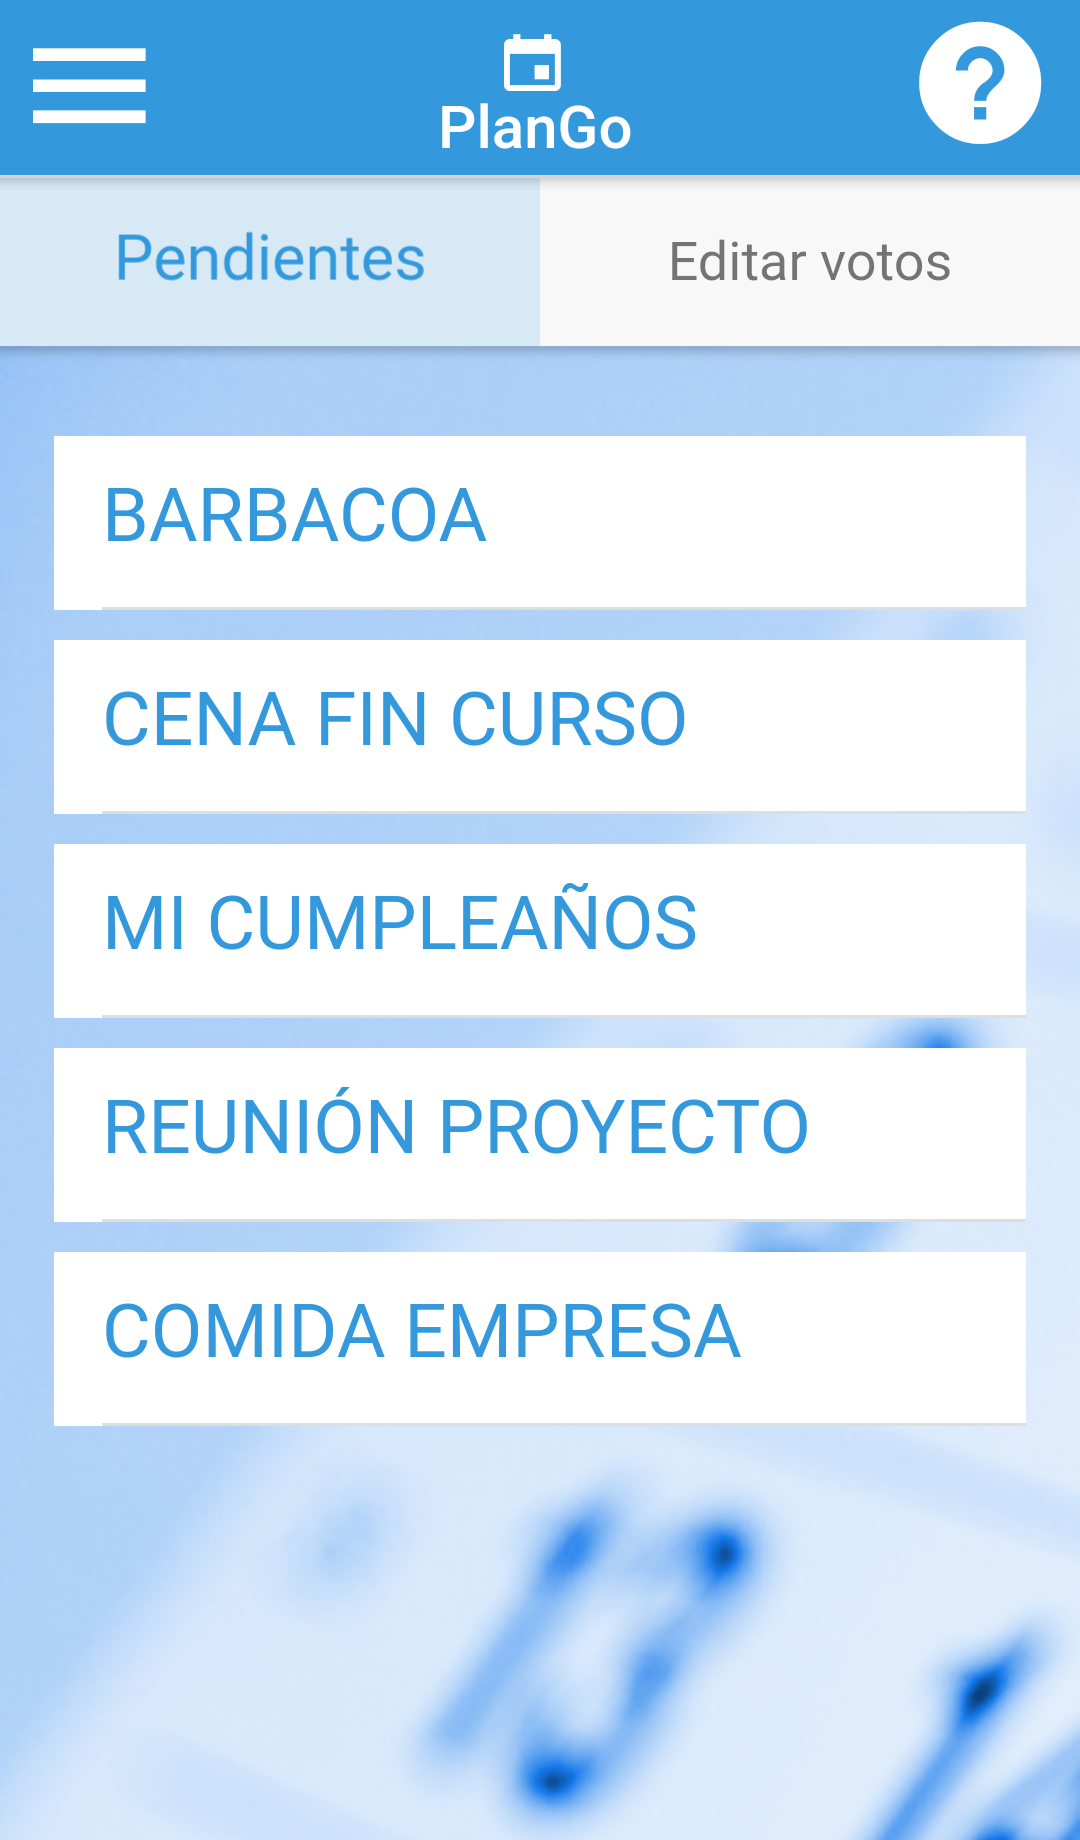
\includegraphics[width=0.3\textwidth]{img/pendientes.png}}
  \subfloat[Votaci\'on]{
   \label{f:votacion}
    
\includegraphics[width=0.3\textwidth]{img/pend.png}}
 \caption{Pantalla de Votaciones pendientes}
 \label{f:votaciones_pendientes}
\end{figure}

Esta pantalla contiene dos tabs. Ambas contienen un listado de encuestas, pero estan destinadas a distinta funcionalidad.

En la tab pendientes (figura \ref{f:pendientes}) se encuentran todas las encuestas que el usuario a\'un no ha votado. Para poder
realizar el voto hay que pulsar encima del t\'itulo de la encuesta. De esta manera se accede al detalle de la encuesta y sus opciones.
Una vez decidido el voto, se pulsa en 'Guardar mi voto'.

En la tab editar voto, aparecen las encuestas que ya han sido votadas. Esta pantalla permite modificar un voto ya enviado. Su funcionalidad
es igual que en el caso de pendientes, al pulsar encima del t\'itulo se accede a la votaci\'on.




\subsection{Arquitectura} 
\label{sec:arquitectura}

La arquitectura general es la de la figura \ref{figura:estructura_ionic} que ya ha sido explicada en el cap\'itulo de introducci\'on en la
tecnolog\'ia Ionic. Como ya hemos dicho, la parte en la que se lleva a cabo todo el desarrollo es en la carpeta 'src', por esto es la parte
en la que voy a entrar en detalle.

\subsubsection{App} 
\label{sec:app}

Existe una carpeta llamada 'app', en la cual lo m\'as importante es:

\begin{itemize}
\item Una carpeta que contiene ficheros destinados a la declaraci\'on de variables para ser usadas en toda la aplicaci\'on. Esta serie de variables son utilizadas en los estilos de los componentes.
Contienen los colores, tama\~nos de letra e iconos. Este es un ejemplo de buenas pr\'acticas, si fuera necesario cambiar la apariencia de toda la aplicaci\'on, bastaria con modificar alguna de estas variables.

\item Fichero app.component.ts: contiene la inicializaci\'on de la aplicaci\'on y configuraci\'on para elegir cu\'al ser\'a la pantalla de inicio.

\item Fichero app.module.ts: tiene gran importancia ya que en \'el est\'an declarados todos los componentes y servicios que han sido creados.

\item Fichero app.css: contiene reglas de CSS que se aplican a todos los componentes.

\end{itemize}

\subsubsection{Pages} 
\label{sec:pages}

En la carpeta 'pages' es donde se encuentran todos los componentes creados. Como se ha visto en el punto \ref{subsec:func_angular}, Angular esta basado en componentes, que ha su vez
pueden contener otros componentes. De esta manera la arquitectura conseguida es m\'as estructurada. 

Cada componente esta formado por tres ficheros: el typescript donde est\'a la l\'ogica, el html donde est\'a la vista y el css que modifica la vista.

En este proyecto, hay pantallas que est\'an formadas \'unicamente por un componente y otras que contienen m\'as. La pantalla de login es la \'unica que realmente contiene un \'unico componente, en cambio Registro, Home y Perfil aparte de su propio componente, est\'an formados por el componente com\'un Header. En la figura \ref{figura:arq_comp}, de forma esquem\'atica, se puede ver qu\'e componentes forman cada una de las pantallas. 

La pantalla de Mis encuestas cuenta con dos diferentes, uno que muestra el listado de todas las encuestas creadas por el usuario logeado  y otro para mostrar el detalle y sus votos. Este \'ultimo contiene a su vez el componente de calendario, que s\'olo se muestra en el caso de ser una encuesta de tipo fecha.

La pantalla de Nueva encuesta est\'a formada por cuatro componentes. Un componente principal que contiene las tabs y el control sobre estas, y los componentes de las pantallas del primer, segundo y tercer paso. El primer paso es la creaci\'on, el segundo la invitaci\'on y por ultimo la pantalla de editar.

La pantalla de Votaciones pendientes, tiene estructura similar a la de Nueva encuesta. Hay un componente principal que contiene las tabs y el control de est\'as, y los dos componentes que forman las pantallas de cada tab.

El componente Header, que es com\'un para la mayoria de las pantallas, lo esta puesto en la figura aparte. Este contiene el men\'u lateral, que es un componente y la navegaci\'on a Ayuda, que tambi\'en es un componente.




\begin{figure}[H]
  \centering
  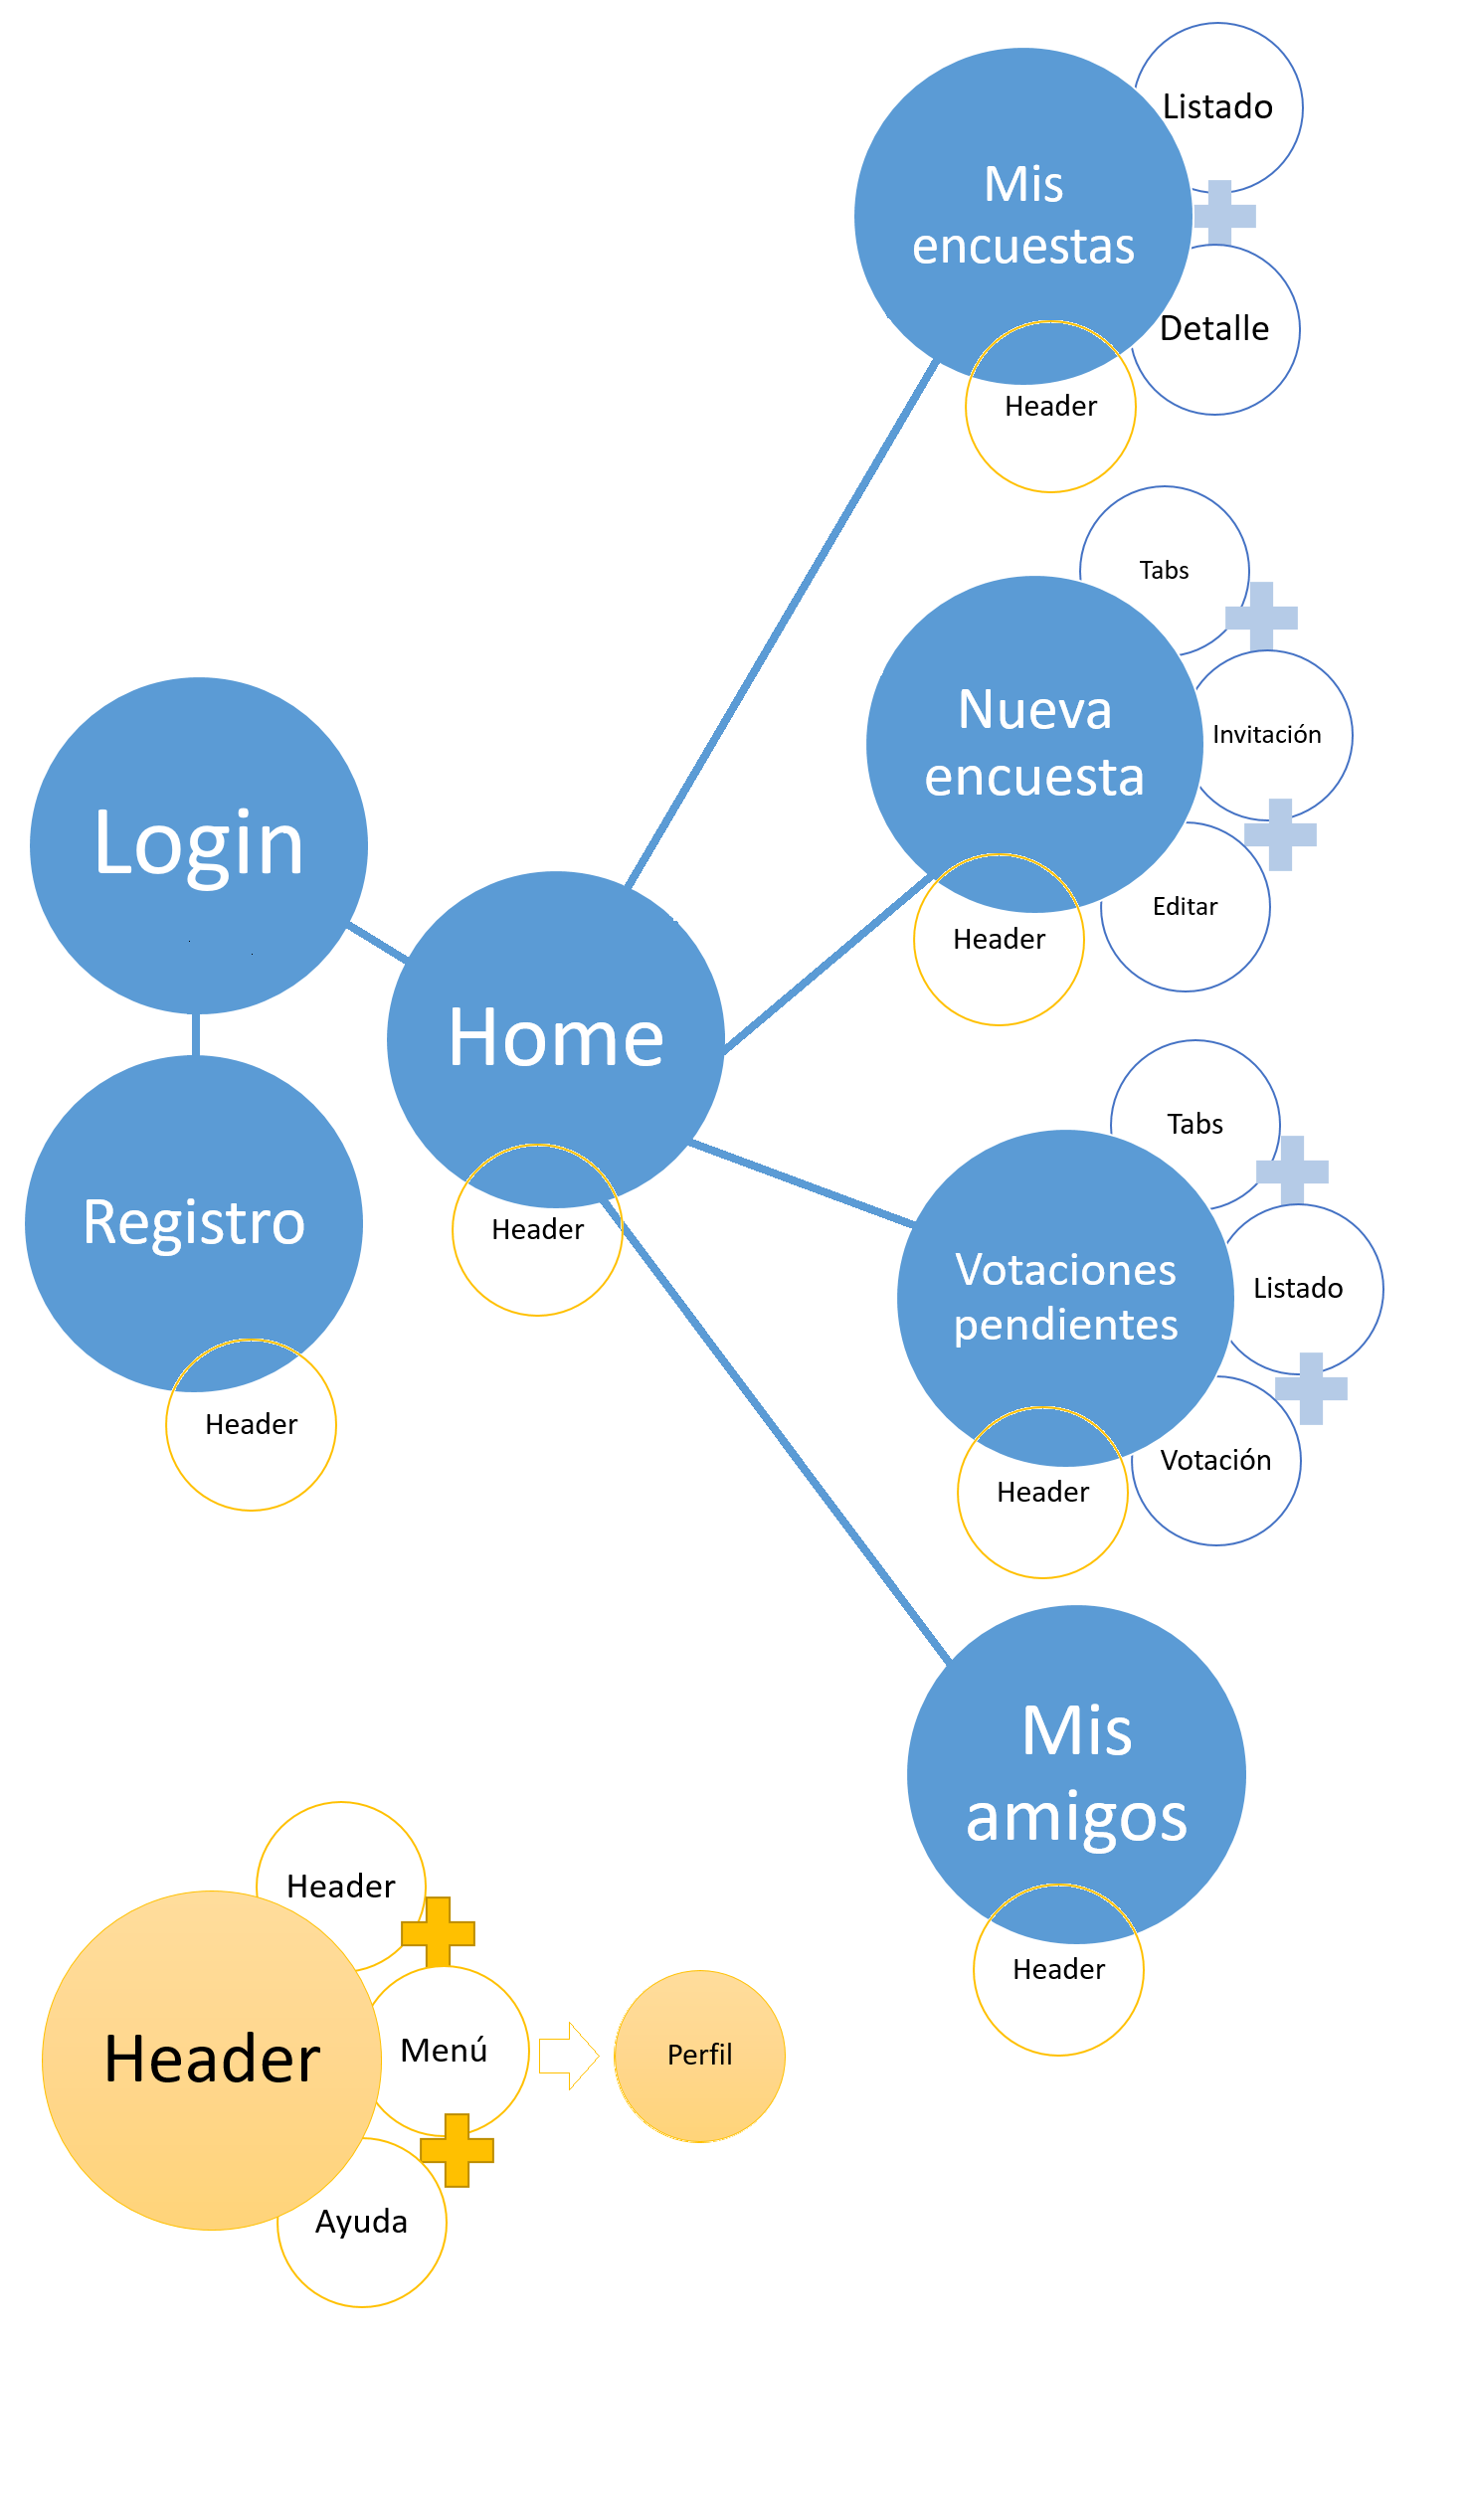
\includegraphics[width=13cm, keepaspectratio]{img/arq_comp.png}
  \caption{Estructura componentes}
  \label{figura:arq_comp}
\end{figure}


\subsubsection{Shared} 
\label{sec:shared}

Esta carpeta ha sido creada para todos los servicios de la aplicaci\'on, componentes comunes y modelos de datos. Los servicios son 
los encargados de hacer la l\'ogica de negocio, asi como las peticiones al servidor. Los modelos son intefaces que definen que atributos
contiene un objeto, de esta forma se protege el c\'odigo contra posibles fallos por mal tipado.

\begin{itemize}
\item Los componentes comunes y por lo tanto, que han sido reusados son el header, el men\'u y el calendario. En el caso del calendario, no es un componente com\'un como tal, ya que solo es utilizado en una pantalla, pero he considerado que debe estar en esta carpeta por estar totalmente preparado para ser rehusado.
\item Los modelos son: friend, poll, user y vote. Es una forma de asegurarnos que las variables que creamos contienen exclusivamente lo que esta declarado en el modelo. Esta es la gran ventaja que tiene TypeScript como ya se ha comentado.

\item Existe un servicio para las peticiones al servidos de cada una de las pantallas. Adem\'as, hay un servicio que contiene toda la l\'ogica de como realizar peticiones HTTP de tipo GET, PUT y POST. Esto facilita que en cada servicio solo sea necesario importar este servicio y despu\'es usarlo para las distintas peticiones que se necesitan.
\end{itemize}


\subsection{Capa de servicios} 
\label{sec:arquitectura}

En este apartado vamos a dejar de lado la parte de la vista de la aplicaci\'on para ir adentr\'andonos en la parte de servicios. Por un lado hay un proyecto para todo el desarrollo de la parte front y otro para la parte back, pero esto tiene que ser conectado de alguna manera. Una vez visto este paso intermedio, profonduzaremos en la parte back en el apartado \ref{sec:backend}.


El cliente env\'ia una petici\'on HTTP, en este caso la aplicaci\'on. La petici\'on es un mensaje de texto creado por un cliente en un formato especial. El cliente env\'ia la petici\'on a un servidor, y luego espera la respuesta. La primera l\'inea de una petici\'on HTTP es la m\'as importante y contiene dos cosas: la URI y el m\'etodo HTTP. La URI es la direcci\'on o ubicaci\'on que identifica un\'ivocamente al recurso que solicita el cliente y el m\'etodo HTTP  define lo que quieres hacer con el recurso.

En la figura \ref{figura:http_service} est\'an representadas todas las peticiones que realiza la aplicaci\'on, separadas por pantallas. El m\'etodo GET se utiliza para recuperar datos del servidor y transmite informaci\'on a trav\'es de la URI agreg\'andole par\'ametros. El m\'etodo POST se usa para crear un recurso en el servidor y los datos se incluyen en el cuerpo de la petici\'on.


\begin{itemize}
\item Login: 
solo es necesario consultar si el usuario y contrase\~na introducidos son correctos y existen en la base de datos. El m\'etodo utilizado para ello es de tipo POST, ya que los detalles de email y contrase\~na se enviar\'an en el cuerpo de mensajes HTTP en lugar de en la URL.

\item Registro:
lo que se quiere es generar un recurso en el servidor, es decir, a\~nadir en la base de datos un nuevo usuario. El m\'etodo utilizado para ello es de tipo POST, en cuyo cuerpo lleva el nombre de usuario, email y contrase\~na.

\item Mis encuestas:
es necesario realizar una petici\'on para recuperar todas las encuestas. Para ello se realiza una peticion GET con el id del usuario como par\'ametro. Adem\'as de esta petici\'on, a la hora de visualizar los votos que tiene determinada encuesta, se utiliza una petici\'on GET con id de encuesta como par\'ametro.

\item Nueva encuesta:
a la hora de crear una encuesta, como ya ha sido explicado en el apartado \ref{sec:nueva_encuesta}, existen tres pasos diferentes, de los cuales, los dos primeros requieren peticiones HTTP. 
En el primer paso, en la creaci\'on de la encuesta, se usa una petici\'on POST para que se a\~nada la encuesta en la base de datos. En el cuerpo de esta petici\'on, van el t\'itulo, las opciones y todos los datos que definen la encuesta. 
Una vez creada la encuesta, en el segundo paso, hay que enviar la encuesta a los amigos. Para pintar el listado de amigos, es necesario traer estos datos del servidor mediante una petici\'on GET con id de usuario como par\'ametro. Adem\'as se utilizan peticiones para a\~nadir o borrar la encuesta al amigo seleccionado.

\item Votaciones pendientes: 
para poder pintar el listado de votos pendientes o de editar votos, se realiza la petici\'on GET correspondiente, que tendr\'a como par\'amento el id del usuario. Para guardar cualquier voto, se hace mediante una petici\'on POST con los votos en el cuerpo.
Si se realiza la votaci\'on de una encuesta que pertenece a los votos pendientes, desaparecer\'a de los votos pendientes y pasar\'a a ser de la lista de editar votos. Todo esto se realiza con peticiones POST.

\item Perfil:
esta pantalla permite los cambios de usuario o de contrase\~na. Ambos se hacen con peticiones PUT, ya que solo se trata de actualizar los valores en la base de datos.

\item Mis amigos:
esta parte de la aplicaci\'on requiere de dos listados. Ambos son obtenidos mediante peticiones GET, cada una apuntando a la URL correspondiente.

\end{itemize}

\begin{figure}[H]
  \centering
  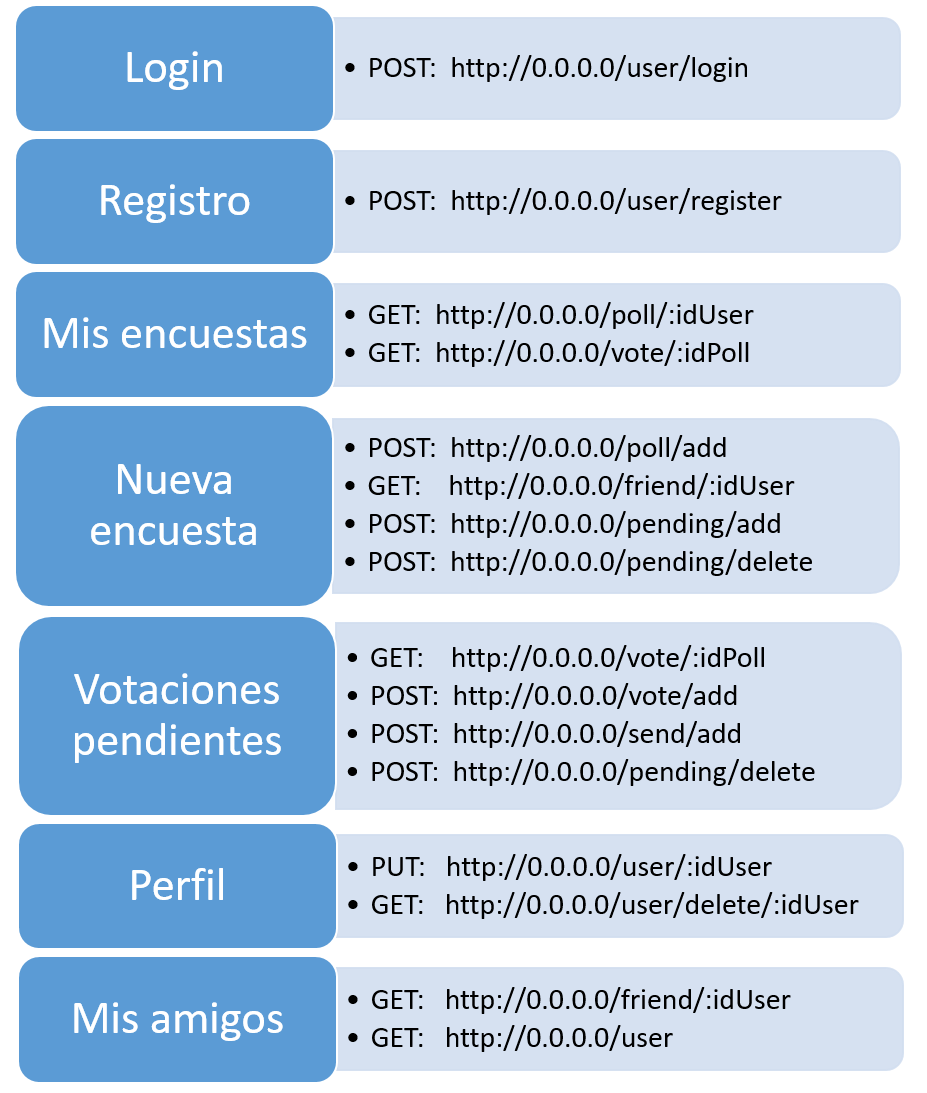
\includegraphics[width=11cm, keepaspectratio]{img/http_service.png}
  \caption{Peticiones HTTP}
  \label{figura:http_service}
\end{figure}



\section{Backend}
\label{sec:backend}

Est\'a enfocado s\'olo a lenguajes de programaci\'on, orientado a funcionamientos, trabajar con datos internos, crear aplicaciones que controlen datos  de la base de datos de la web, para poder ser consultados por el usuario.

Toda la parte \emph{backend} esta desarrollada con las tecnolog\'ias Express y MongoDB. 


\subsection{Servidor} 
\label{sec:servidor}

Un servidor es un ordenador u otro tipo de equipo inform\'atico encargado de suministrar informaci\'on a una serie de clientes, que pueden ser tanto personas como otros dispositivos conectados a \'el. 

En este proyecto se han utilizado servicios REST, que ha sido explicado en el apartado \ref{subsec:rest}.

El servidor esta desarrollado con un framwork llamado Express, cuyos detalles ya han sido explicados en el apartado \ref{subsec:express}. 

Existe un fichero llamado 'app.js' para la creaci\'on del servidor y por lo tanto hacer llamadas HTTP. En este fichero se encuentran las dependencias necesarias. Tambien se encuentra que con HTTP se crea el servidor y se le indicamos en que IP y puerto estar\'a escuchando. A esta direcci\'on donde la parte del cliente enviar\'a las peticiones. Todo esto es parte de la configuraci\'on necesaria para la creaci\'on de un servidor.

Una vez creado el servidor, se declaran las rutas con sus correspondientes m\'etodos HTTP e instancias. Esto significa qu\'e cuando el servidor reciba una petici\'on con alguna de las rutas declaradas y con el correcto m\'etodo, se llevara a cabo la instancia que est\'a indicada para dicha ruta. En la figura \ref{f:ej_route} se puede ver un ejemplo de como se crean las rutas.

Aparte de esto, falta una parte importante, la conexi\'on con la base de datos, en este caso con MongoDB.

En los siguientes apartados, se detallan los modelos y controladores, estos tambi\'en son importados en el fichero 'app.js' para su uso.

\begin{figure}[H]
  \centering
  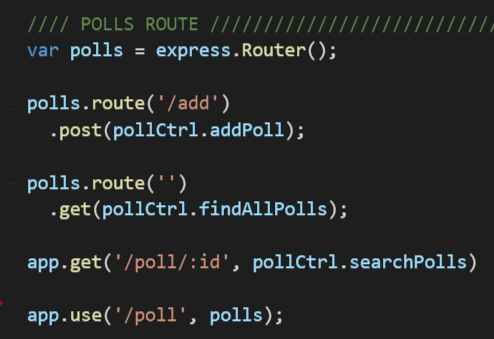
\includegraphics[width=8cm, keepaspectratio]{img/ej_route.png}
  \caption{Ejemplo: ruta encuestas}
  \label{f:ej_route}
\end{figure}



\subsection{Modelos} 
\label{sec:modelos}

Los modelos son creados usando Mongoose para poder guardar la informaci\'on en la base de datos siguiendo el esquema. Como base de datos se ha utilizado MongoDB. Al ser una base de datos Open Source NoSQL orientada a documentos tipo JSON viene bien para entregar los datos en este formato en las llamadas a la API. 

Los modelos que han sido creados son:
\begin{itemize}
\item User: contiene la informaci\'on necesaria del usuario: el nombre, email y contrase\~na.
\item Poll: contiene la informaci\'on de una encuesta: titulo, ubicaci\'on, comentario, si solo es posible un voto, las opciones, el tipo de encuesta y el id del usuario que la ha creado. Ver figura \ref{f:ej_model}
\item Friend: contiene el id del usuario y los usuarios que son sus amigos.
\item Vote: contiene el id de la encuesta y las opciones con sus respectivos votos.
\item Pending-vote: contiene un id de usuario y las encuestas que tiene dicho usuario por votar.
\item Send-vote: contiene un id de usuario y las encuestas dicho usuario ya ha votado. 
\end{itemize}

Una vez creados los modelos, se puede implementar la conexi\'on a la base de datos en el archivo antes explicado, 'app.js'.

\begin{figure}[H]
  \centering
  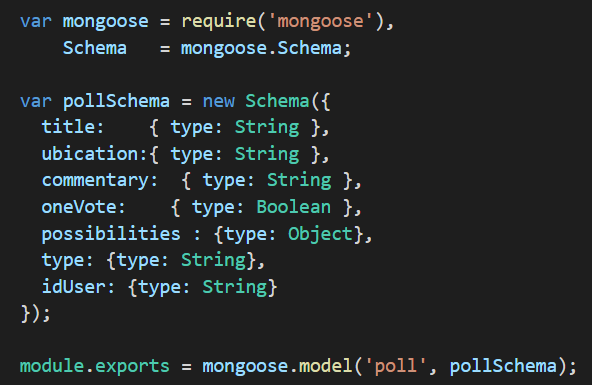
\includegraphics[width=9cm, keepaspectratio]{img/model.png}
  \caption{Ejemplo: modelo encuesta}
  \label{f:ej_model}
\end{figure}


\subsection{Controladores} 
\label{sec:controladores}

La parte de controlador tiene mucho que ver con el enrutamiento y con lo que en Express llaman \emph{middleware}: funciones que reciben una entrada (request) y una salida (response). Lo que sucede entre la entrada y la salida es el controlador.

Los controladores de las rutas de la API est\'an creados en un archivo separad que se llama 'controllers'. Estos controladoes son exportados para poder modularizarlos y que puedan ser llamados desde el archivo principal de la aplicaci\'on. 

Existe un controlador por cada modelo de datos, en cada uno de los cuales existen funciones para llevar a cabo diferentes interaciones con la base de datos. Las interaciones suele ser que a\~nadir datos, actualizarlos o eliminarlos.

En todos los controladores existen unas funciones que son comunes para todas pero con sus correspondientes peculiaridades:

\begin{itemize}
\item 'FindAll...': realiza una b\'usqueda por la colecion de la base de datos que se le haya indicado. Devuelve todos los datos encontrados, sin ning\'un filtro.

\item 'FindById': como su propio nombre indica, realiza una b\'usqueda por la colecion de la base de datos que se le haya indicado y devuelve solo aquellos datos filtrados por un ID.

\item 'Add...': funci\'on utilizada para a\~nadir datos a la colecci\'on indicada. Esta funci\'on no coincide en todos los controladores. En el caso del controlador para usuarios, antes de a\~nadir un nuevo usuario se comprueba que no haya ningun usuario con el mismo nombre ni con el mismo email. En los dem\'as controladores, se comprueba si el dato a a\~nadir ya existe en la base de datos, para actualizarlo o a\~nadirlo.

\item 'Search...': realiza una b\'usqueda por la base de datos. En cada uno de los controladores dicha b\'usqueda se realiza por el dato o datos que repesentan el modelo de datos. En el caso del controlador de usuarios se busca por email y contrase\~na y en el resto se busca por el id de usuario.

\item 'Update...': como su nombre indica, sirve para actualizar datos en la base de datos sobre algo ya almacenado.

\item 'Delete...': permite eliminar datos de la base de datos.

\end{itemize}

\begin{figure}[H]
  \centering
  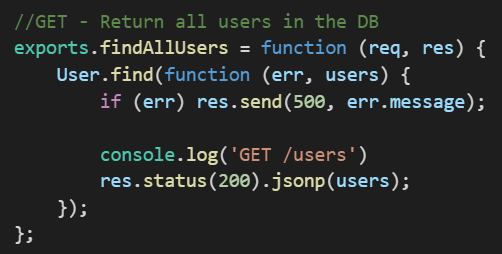
\includegraphics[width=9cm, keepaspectratio]{img/controller.png}
  \caption{Ejemplo: funci\'on controlador}
  \label{f:controller}
\end{figure}

Siempre que se quiera trabajar con los datos de una base de datos debe
seguir una nomenclatura definida. Primeramente aparece el nombre de la colecci\'on sobre la que se quiere
trabajar y posteriormente el m\'etodo a usar. Los m\'etodos usados para filtrar han sido findById para filtrar por id, findOne para buscar un dato concreto. Para introducir o eliminar datos se han usado otros m\'etodos: 'save' y para borrar 'detele'.


\subsection{Base de datos: MongoDB} 
\label{sec:base_datos_mongo}

\begin{figure}[H]
  \centering
  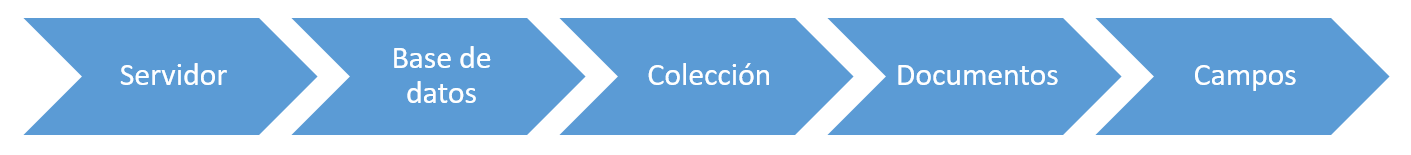
\includegraphics[width=14cm, keepaspectratio]{img/arq_mongo.png}
  \caption{Arquitectura MongoDB}
  \label{f:arq_mongo}
\end{figure}

La jerarqu\'ia principal de MongoDB viene dada por los elementos
presentados en la figura \ref{f:arq_mongo}. Utiliza documentos con distintas estructuras. Un
conjunto de Campos formar\'an un Documento, que en caso de asociarse con
otros formar\'a una Colecci\'on. Las bases de datos estar\'a formada por
Colecciones, y a su vez, cada servidor puede tener tantas bases de datos como el
equipo lo permita.

En este caso solo hay una base de datos, que recibe el nombre de encuestasApp. Esta base de datos tiene seis coleccioneque contienen  una serie de campos diferentes, en funci\'on de las necesidades de dicha colecci\'on. Estas funcionalidades se ver\'an detalladamente en el apartado \ref{sec:colecciones}.

En la figura \ref{f:ej_col}, se puede ver en detalle como esta formada la base de datos. Aparecen todas las colecciones y en detalle la de 'Users'. Esta colecci\'on almacena Documentos con los campos de usuario, email y contrase\~na, adem\'as a\~nade campo de id que identifica este documento en la base de datos y campos propios de la encriptaci\'on. 

\begin{figure}[H]
  \centering
  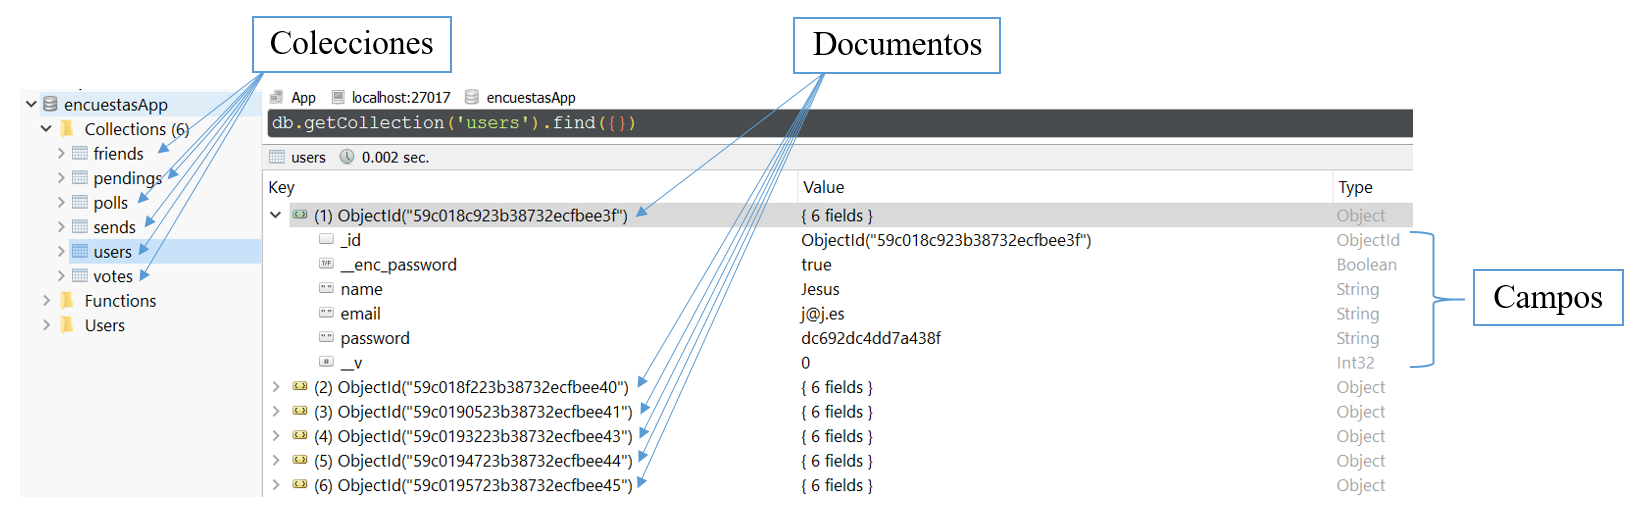
\includegraphics[width=17cm, keepaspectratio]{img/ej_col.png}
  \caption{Ejemplo coleccion 'Users'}
  \label{f:ej_col}
\end{figure}


\subsection{Colecciones} 
\label{sec:colecciones}

Una colecci\'on, como ya se ha explicado, es un contenedor de los documentos en MongoDB. No es necesaria su creaci\'on datos por primera vez, ya que Mongo comprueba previamente si existe la colecci\'on y si no, la crea autom\'aticamente.

Todos los documentos tienen el capo de 'id', este campo es creado por Mongo para poder identificar cada documento y 'v' que hace refecencia a la versi\'on.

\subsubsection{Users} 
\label{sec:c_users}
Esta coleci\'on contiene documentos con los campos de nombre, email, contrase\~na. Adem\'as, tambi\'en existen el campo 'encpassword', que nos permite saber si la contrase\~na esta o no encriptada.

La principal funci\'on de esta coleci\'on es almacenar todas las cuentas de usuario que se han creado en la aplicaci\'on. Solo aquellos usuarios que tengan cuenta podr\'an acceder, introduciendo su email y contrase\~na. Adem\'as de esto, nos d\'a un identificador que es \'unico para cada usuario. Este id es muy importante a la hora de relacionar los datos de esta colecci\'on con otra.

\subsubsection{Polls} 
\label{sec:c_polls}
Esta coleci\'on contiene documentos con los campos de t\'itulo, ubicaci\'on, comentario, solo un voto, tipo, opciones e id de usuario.

Todas las encuestas que son creadas a trav\'es de la aplicaci\'on son almacenadas en esta colecci\'on. Para saber quien es el creador de la encuesta, cada documento contine el campo 'idUser', este coincide con uno de los id de la colecci\'on de 'Users'. De esta manera tenemos relacionadas ambas colecciones.

\subsubsection{Friends} 
\label{sec:c_friends}
Esta coleci\'on contiene documentos con los campos de id de usuario e id de amigos.

El id de usuario se corresponde a un id de la colecci\'on de 'Users' y nos permite conocer a qu\'e usuario estamos haciendo referencia. El id de amigos se trata de un array de ids, todos ellos de la coleccion de 'Users. De esta forma, cuando se necesita conocer qu\'e amigos tiene un determinado usuario, solo es necesario filtrar esta colecci\'on por su id y, a partir de su array id de amigos y la colecci\'on 'Users', conocer los detalles de sus amigos. 

\subsubsection{Votes} 
\label{sec:c_votes}

Esta colecci\'on contiene documentos con los campos de id de encuesta y un array de opciones. Dentro de este array, hay otro array que contiene los voto.

El id de encuesta se corresponde a un id de la colecci\'on de 'Polls' y nos permite saber a que encuesta estamos haciendo referencia. El array de opcione contiene todas las opciones de la encuesta. Por cada opci\'on hay un array en el que se almacena quien la ha votado. 


\subsubsection{Pendings} 
\label{sec:c_pending}

Esta colecci\'on contiene documentos con los campos de id de usuario e id de encuesta.

La funcionalidad de esta colecci\'on es conocer que encuestas tiene el usuario pendientes de votar. Con el id de usuario se conoce el usuario que tiene que votar y con el id de encuesta la encuesta a votar. Accediendo a la colecci\'on 'Polls' con el id se pueden conocer los detalles de la encuesta.

\subsubsection{Send} 
\label{sec:c_send}

Esta colecci\'on contiene documentos con los campos de id de usuario e id de encuesta.

La funcionalidad de esta colecci\'on es conocer que encuestas ha votado ya el usuario. Con el id de usuario se conoce el usuario que ha votado y con el id de encuesta la encuesta. Accediendo a la colecci\'on 'Polls' con el id se pueden conocer los detalles de la encuesta.


\subsection{Relaci\'on entre colecciones} 
\label{sec:colecciones}

\begin{figure}[H]
  \centering
  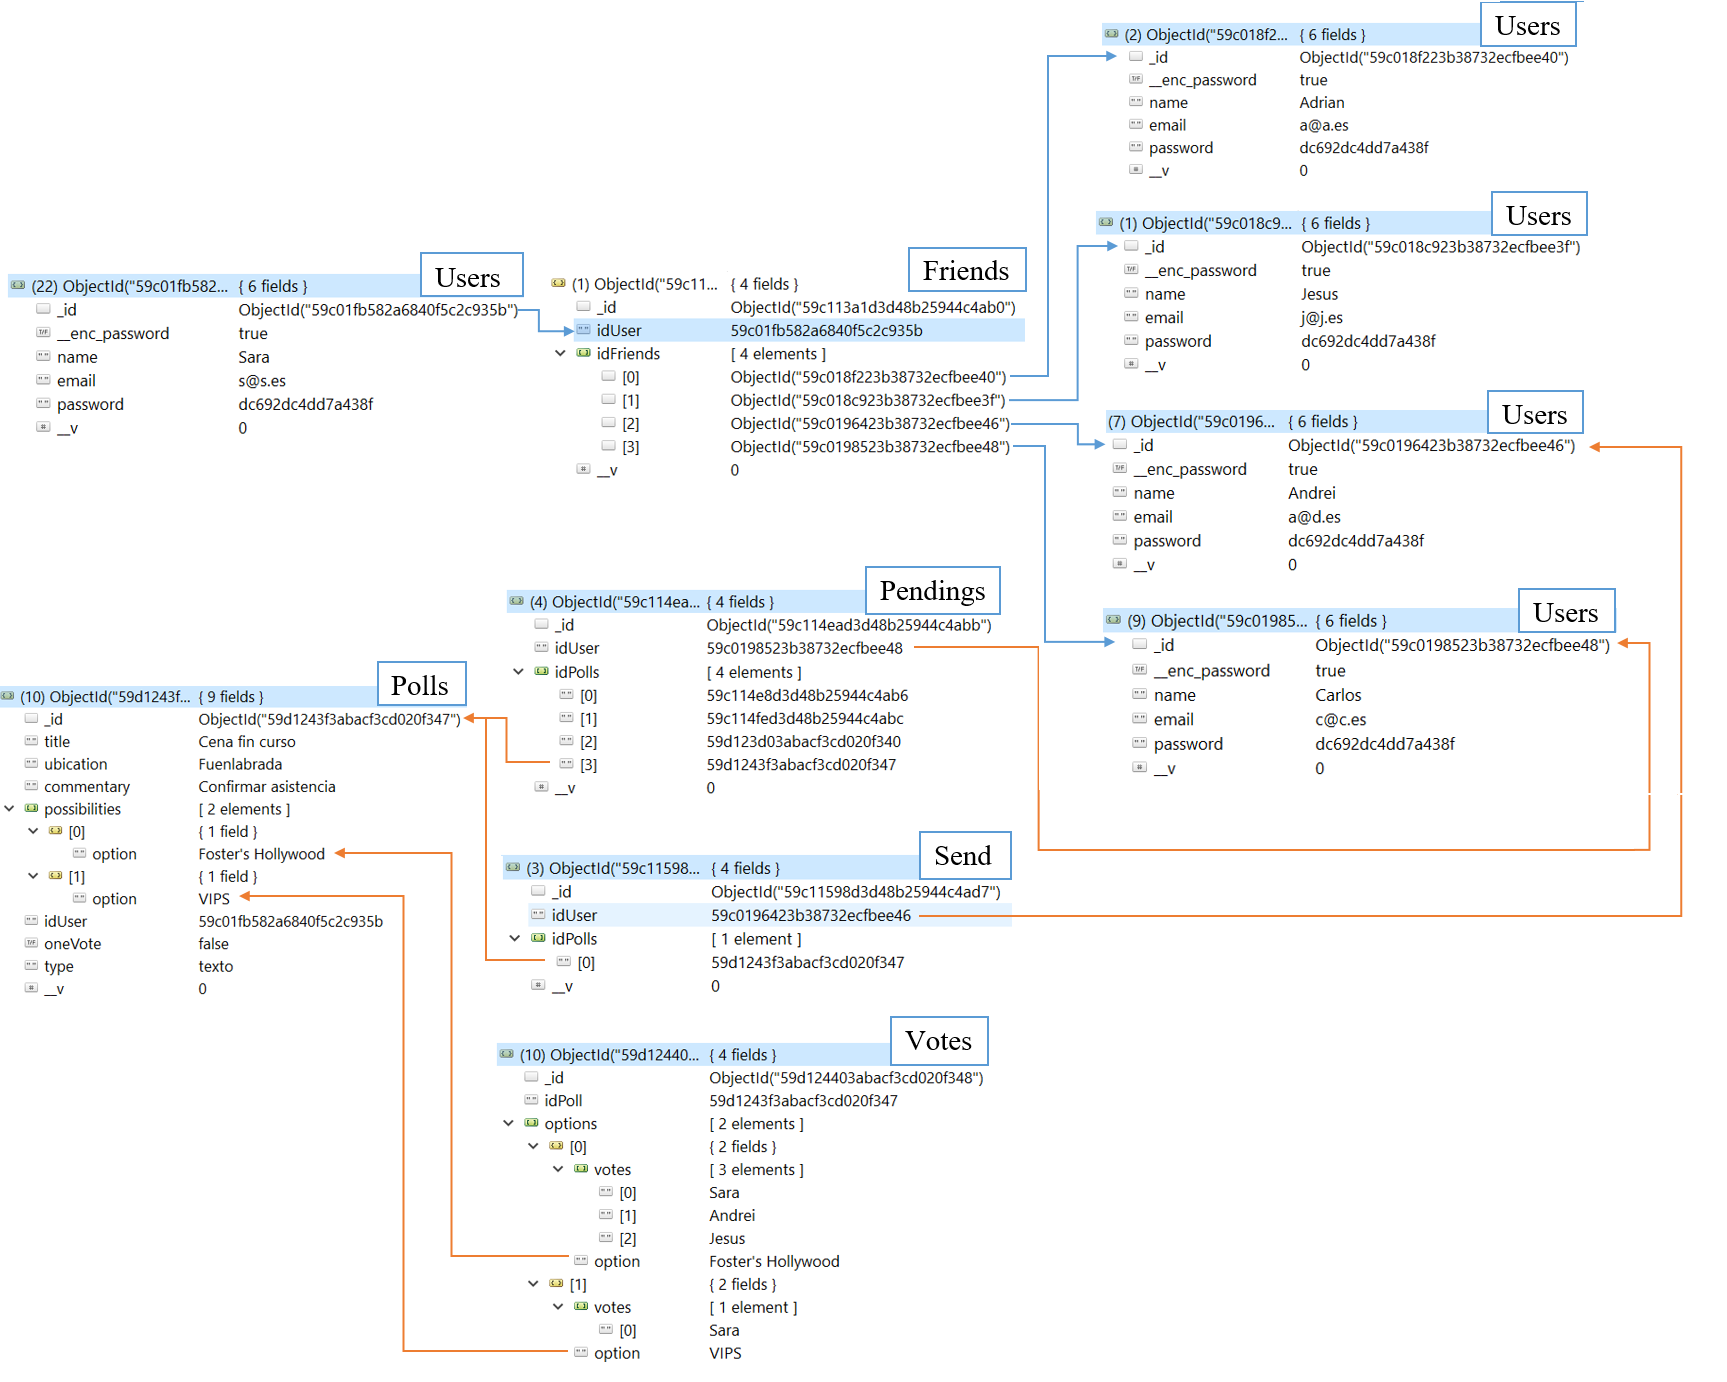
\includegraphics[width=18.5cm, keepaspectratio]{img/base_datos.png}
  \caption{Relaci\'on entre colecciones}
  \label{f:}
\end{figure}

La mejor manera de entender las colecciones descritas en el apartado \ref{sec:colecciones} es saber las relaciones que hay entre ellas. Algunas de las colecciones tienen la funcionalidad unicamente de relacionar dos colecciones. Es el caso de 'Friends', 'Pendigns' y 'Send'. Esto se consigue gracias a los identificadores \'unicos de cada documento.

Esta forma de relacionar datos tiene un inconveniente, la posible inconsistencia de datos. Una base de datos est\'a inconsistente si dos datos que deber\'ian ser iguales no lo son. Esto puede ocurrir si para una funcionalidad se necesita modificar dos colecciones distintas y, por alg\'un error, solo se realiza en una. Al tratarse de una base de datos no relacional, para solucionar esta incosistencia, una coleccion deber\'ia contener todos los datos. Pero esto no ser\'ia eficiente, las operaciones con la base de datos llevar\'ian m\'as tiempo, incluso llegando a ser imposible su uso si el n\'umero de documentos es muy grande.




\subsection{Seguridad} 
\label{sec:seguridad}

La seguridad de aplicaciones web es una rama de la Seguridad Inform\'atica que se encarga espec\'ificamente de la seguridad de sitios web, aplicaciones web y servicios web. Es una rama muy amplia que requerir\'ia una amplia investigaci\'on y aprendizaje. El objetivo de este trabajo no es este, por lo que la seguridad aplicada es bastante b\'asica.

De los datos almacenados en la base de datos, la autentificaci\'on es lo m\'as importante de cara a la seguridad. Por esto he considerado necesario guardar la contrase\~na encriptada. De esta manera, aunque alguien acceda a la base de datos, no podr\'a obtener la contrase\~na real.

La encriptaci\'on est\'a hecha mediante un plugin de mongoose llamado mongoose-field-encryption. Ofrece un cifrado sim\'etrico para campos individuales. En necesario indicar una contrase\~na que permite en encriptado y desencriptado. El inconveniente de este m\'etodo es que si alguien consiguiera esta contrase\~na tendr\'ia acceso a todas las contrase\~nas.

\begin{figure}[H]
  \centering
  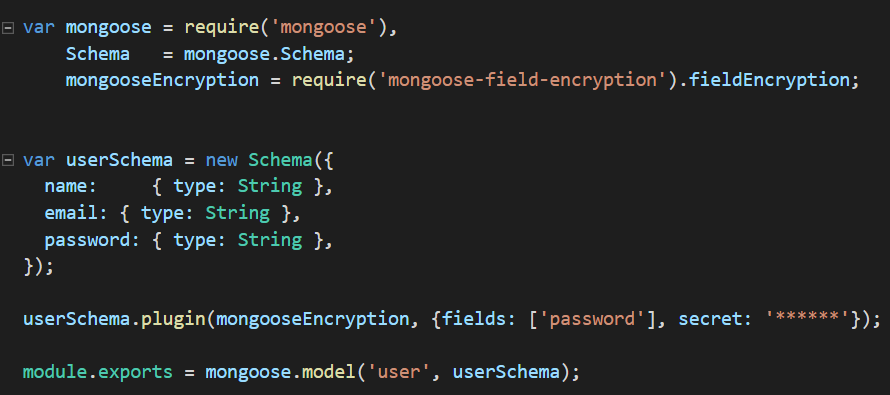
\includegraphics[width=12cm, keepaspectratio]{img/enc.png}
  \caption{Encriptaci\'on}
  \label{f:}
\end{figure}





%%%%%%%%%%%%%%%%%%%%%%%%%%%%%%%%%%%%%%%%%%%%%%%%%%%%%%%%%%%%%%%%%%%%%%%%%%%%%%%%
%%%%%%%%%%%%%%%%%%%%%%%%%%%%%%%%%%%%%%%%%%%%%%%%%%%%%%%%%%%%%%%%%%%%%%%%%%%%%%%%
% PRUEBA %
%%%%%%%%%%%%%%%%%%%%%%%%%%%%%%%%%%%%%%%%%%%%%%%%%%%%%%%%%%%%%%%%%%%%%%%%%%%%%%%%

\cleardoublepage
\chapter{Prueba}

En esta \'ultima fase del proyecto, he realizado una prueba de usuarios con la \'utlima versi\'on de la aplicaci\'on desarrollado. El prop\'osito de esta es comprobar la experiencia de los usuarios, verificar los objetivos que han sido logrados y que no existen fallos en la aplicaci\'on. 

El proceso de beta testing es el \'ultimo paso necesario para disfrutar de una aplicaci\'on que realmente funciona dentro de cualquiera de las tiendas de aplicaciones de las grandes tecnol\'ogicas. En Android el sistema para la subida de una versi\'on de prueba se llama alpha y betta, pero en el caso de iOS se llama TestFlight. Esto es lo que estamos realizando con esta prueba final del proyecto, sin utilizar las plataformas oficiales de Android y Apple.

\section{Objetivos de la prueba} 
\label{sec:seguridad}

El objeto principal de la prueba es la obtenci\'on de resultados sobre la usabilidad y funcionalidad de los usuarios con la aplicaci\'on. Para que una aplicaci\'on sea de inter\'es, es importante que cumpla dichos requisitos.

Para ello se determina si se cumplen los siguientes objetivos:
\begin{itemize}
\item La aplicaci\'on debe cumplir la funcionalidad descrita en los requisitos establecidos inicialmente en la secci\'on \ref{chap:objetivos}.
\item El usuario debe intuir con facilidad como debe utilizar la aplicaci\'on, asi como la navegaci\'on.
\end{itemize}

\section{Desarrollo} 
\label{sec:seguridad}

Para poder desarrollar la prueba ha sido necesario que cada usuario contara con un dispositivo movil. He instalado la aplicaci\'on en cada uno de los dispositivos, con la configuraci\'on correcta para que conecte con el servidor. Dado que la parte \emph{backend} no esta corriendo en ning\'un servidor real, he utiilizado el propio ordenador como servidor.

Una vez acabado esto y con la aplicaci\'on preparada para funcionar, se ha empezado con la prueba. Esta est\'a formada por varias partes. En una primera parte he considerado que ser\'ia interesante dejar a los usuarios navegar por la aplicaci\'on para as\'i valorar como es de intuitiva. En una segunda fase, he marcado una serie de hitos a realizar:

\begin{enumerate}
\item Crear una cuenta.
\item Logearse.
\item Navegar por todos los accesos de la aplicaci\'on para comprobar que no continen ning\'un dato.
\item A\~nadirse como amigos.
\item Crear una encuesta e invitar a los amigos.
\item Votar las encuestas pendientes
\item Cambiar datos del perfil.
\end{enumerate}

En la tercera y \'utima fase, han tenido que rellenar una encuesta en la que debian poner una puntuaci\'on sobre diez a algunos puntos de la aplicaci\'on. Con los resultados de estas preguntas he conseguido llegar a unas conclusiones.

\section{Conclusiones de la prueba} 
\label{sec:conclusion_prueba}

Una vez realizada la prueba, he considerado que los puntos m\'as importantes sobre una aplicaci\'on son: el dise\~no (como de atractivo parece el aspecto visual), la usabilidad (si la aplicaci\'on funciona de forma fluida), la utilidad (si la usarian o no) y la intuitividad (manejo de la app sin ayuda).

Gracias a la primera fase de la prueba, los usuarios pueden reflexionar sobre como de intuitiva es la aplicaci\'on. Respecto a los demas puntos de inter\'es, los usuarios lo han podido sacar sobre el desarrollo de toda la prueba.

En la figura \ref{f:prueba_result} se pueden ver las puntuaciones que ha dado cada usuario. Dado que el n\'umero de usuarios que han realizado la prueba no es alto, los resultados obtenidos no son demasiado relevantes, pero si son suficientes para obtener una idea sobre la opini\'on que pueden tener los usuarios sobre la aplicaci\'on.

\begin{figure}[H]
  \centering
  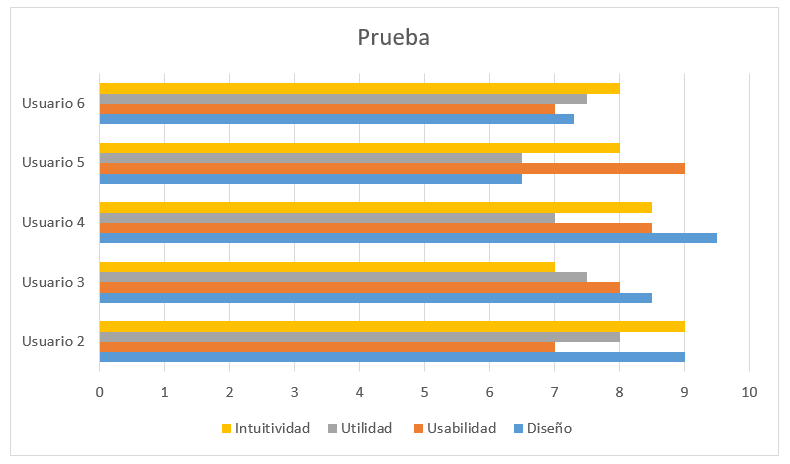
\includegraphics[width=12cm, keepaspectratio]{img/prueba.png}
  \caption{Resultado prueba}
  \label{f:prueba_result}
\end{figure}

Como conclusi\'on se obtiene que los puntos fuertes de la aplicacion son el dise\~no y la intuitividad. El punto a mejorar ser\'ia la utilidad, aunque a\'un as\'i tampoco tiene mal puntuaci\'on. Creo que al ser una aplicaci\'on con una funcionalidad ya conocida por los usuarios, no llama la atenci\'on especialmente por lo que ha podido repercutir en la nota sobre este punto. En cuanto la usabilidad, creo que la nota obtenia es bastante correcta. 

Tras este estudio, creo que ser\'ia interesante pensar una funcionalidad que sorprenda al usuario y que no este acostumbrado a ver.

\begin{figure}[H]
  \centering
  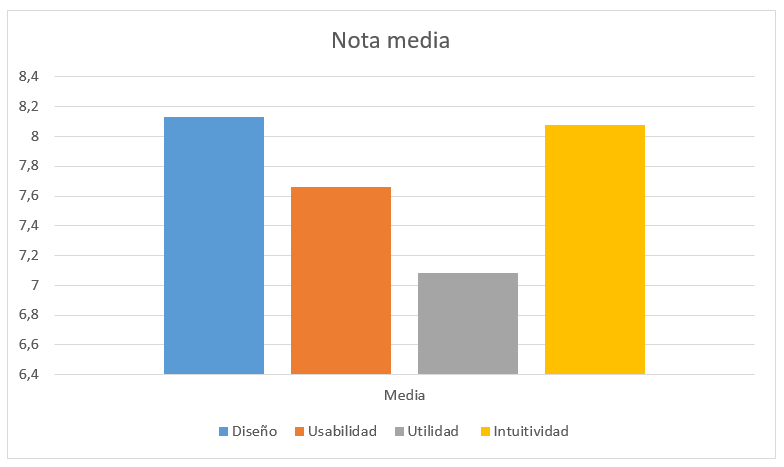
\includegraphics[width=10cm, keepaspectratio]{img/media.png}
  \caption{Media resultado prueba}
  \label{f:prueba-media}
\end{figure}






%%%%%%%%%%%%%%%%%%%%%%%%%%%%%%%%%%%%%%%%%%%%%%%%%%%%%%%%%%%%%%%%%%%%%%%%%%%%%%%%
%%%%%%%%%%%%%%%%%%%%%%%%%%%%%%%%%%%%%%%%%%%%%%%%%%%%%%%%%%%%%%%%%%%%%%%%%%%%%%%%
% CONCLUSIONES %
%%%%%%%%%%%%%%%%%%%%%%%%%%%%%%%%%%%%%%%%%%%%%%%%%%%%%%%%%%%%%%%%%%%%%%%%%%%%%%%%

\cleardoublepage
\chapter{Conclusiones}
\label{chap:conclusiones}
 
\section{Planificaci\'on temporal}
\label{sec:planificacion-temporal}

El tiempo empleado la finalizaci\'on de este proyecto ha sido de cinco meses naturales, de los cuales la dedicaci\'on solo ha podido ser ha tiempo parcial. La media de horas empleadas al d\'ia entre semana ha podido ser, aproximadamente, de tres horas y los fines de semana una media de cinco horas. 

El proyecto ha pasado por varias fases a lo largo del tiempo:

\begin{itemize}
\item Primer mes:

 Mi dedicaci\'on durantes este tiempo fue a la realizaci\'on de un tutorial sobre Angular\cite{TutorialAngular}, el cual me di\'o una serie de conocimientos para poder empezar la parte visual de la aplicaci\'on. Tras este tutorial, empec\'e a crear las primeras pantallas de la aplicaci\'on.

 \item Segundo mes: 

Este mes fue dedicado a la realizaci\'on de un tutorial destinado a conectar Angular con Meteor para poder desarrollar la parte \emph{backend} con Meteor. Durante este periodo, debido a una serie de problemas con la realizaci\'on de este tutorial, decid\'i buscar otra alternativa y as\'i poder avanzar en el proyecto. Finalmente la tecnolog\'ia elegida fue Express y para empezar el desarrollo segu\'i un tutorial\cite{TutorialExpress}. Esto me permiti\'o poder realizar las primeras llamadas HTTP desde la parte \emph{frontend} de la aplicaci\'on.

\item Tercer y cuarto mes: 

Una vez montada la base de la parte front y la parte back, desarrolle en paralelo ambas partes. Desarrollaba la pantalla y a la par,  creaba los controladores necesarios en Express para que atendiera a las peticiones necesarias en dicha pantalla. Una vez terminado todo el desarrollo, fue importante la parte del testeo de la aplicaci\'on. Durante esta parte se cambiaron funcionalidades de la aplicaci\'on como: poder a\~nadir hora como opci\'on en una encuesta, ordenar alfab\'eticamente los listados, cambio en pantalla de visualizo de votos, etc.

\item Quinto mes: 

Este \'ultimo tramo ha sido dedicado a la elaboraci\'on de la memoria y la preparaci\'on de la presentaci\'on. Adem\'as de esto, durante esta etapa, se hizo el experimento de poner a un grupo de personas a usar la aplicaci\'on siguiendo una serie de hitos, para posteriormente contestar unas preguntas.

\end{itemize}

\section{C\'odigo fuente}
\label{sec:codigo-fuente}

El c\'odigo fuente de la aplicaci\'on se encuentra en repositorios de GitHub. Existen tres repositorios para este trabajo: uno para el proyecto de  \emph{frontend}, otro para el proyecto de  \emph{backend} y por \'ultimo uno para la memoria desarrollada en Latex. Utilizar esta herramienta permite tener un buen control de versiones.

El proyecto \emph{frontend} se encuentra en:

 \url{https://github.com/LopezZambrano/prueba/tree/master/planGO}.

El proyecto \emph{backend} se encuentra en:

 \url{https://github.com/LopezZambrano/node-api-rest}. 

La memoria se encuentra en:

 \url{https://github.com/LopezZambrano/memoria-planGO}.

\subsection{M\'etrica LOC}
\label{sec:metrica-fuente}

El n\'umero de l\'ineas de c\'odigo o LOC\cite{LOC} (\emph{Lines Of Code}) es una m\'etrica est\'andar que se utiliza para tratar de determinar el tama\~no de un desarrollo inform\'atico y tambi\'en en cierta medida dan una idea del esfuerzo que se ha necesitado para crearlo.

Las LOC son una medida un tanto imprecisa, porque se puede escribir c\'odigo m\'as o menos compacto seg\'un el estilo de cada uno. Adem\'as hay lenguajes con sintaxis m\'as larga que otras y por tanto que generan m\'as l\'ineas.

Adem\'as de l\'ineas de c\'odigo en total es interesante medir tambi\'en algunas m\'etricas relacionadas, como las que han sido medidas en este caso: n\'umero de ficheros, espacios en blanco y comentarios.

Dado que se han utilizado frameworks que generan codigo de forma autom\'atica, solo ha sido contabilizado aquel c\'odigo que ha tenido que ser desarrollado. De esta manera el an\'alisis se ajusta m\'as al esfuerzo realizado.

Para realizar este an\'alisis, se ha utilizado una herramienta llamada CLOC\cite{CLOC}. Los resultados obtenidos en dicho an\'alisis han sido recogidos las tablas de las figuras \ref{f:front-media} y \ref{f:back-media}.

Las conclusi\'on de este an\'alisis, viendo los resultados, es clara. Existe un mayor exfuerzo en la parte de \emph{frontend} con un total de 4.419 l\'ineas de c\'odio frente a las 559 de la parte de \emph{backend}.

\begin{figure}[H]
  \centering
  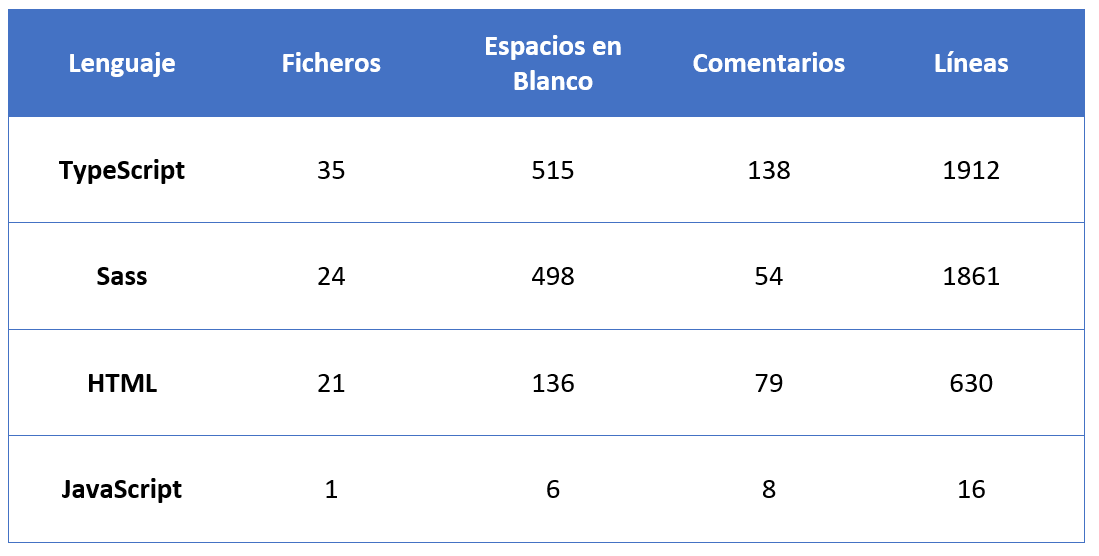
\includegraphics[width=12cm, keepaspectratio]{img/front_a.png}
  \caption{An\'alisis c\'odigo frontend}
  \label{f:front-media}
\end{figure}

\begin{figure}[H]
  \centering
  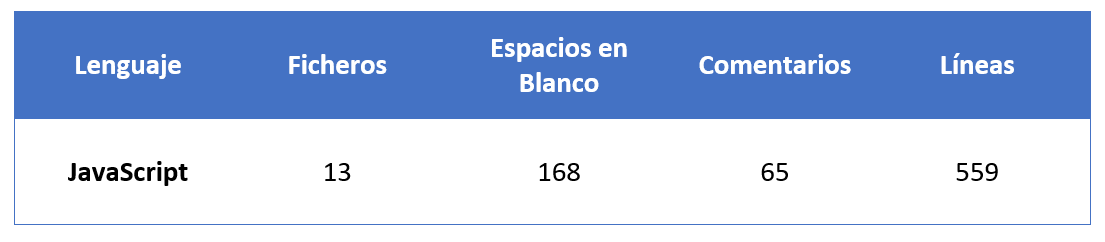
\includegraphics[width=12cm, keepaspectratio]{img/back_a.png}
  \caption{An\'alisis c\'odigo backend}
  \label{f:back-media}
\end{figure}





\section{Aplicaci\'on de lo aprendido}
\label{sec:aplicacion}

El principal conocimiento que se ha aplicado para el desarrollo de este trabajo es el de la proramaci\'on. Durante todos los a\~nos del grado se ha ido mejorando este conocimiento practicando con diferentes lenguajes. Tambi\'en es importante el desarrollo personal durante estos a\~nos de ser autodidacta, lo que da cierta soltura para aprender nuevos lenguajes. 

Durante el grado de Ingenier\'ia en Sistemas de Telecomunicaci\'on, s\'olo he tenido una asignatura relacionada con este proyecto. Esta asignatura se llama Servicios y Aplicaciones de Ordenadores. En esta asignatura desarrollamos una p\'agina web sobre indicencias de tr\'afico. Esta pr\'actica fu\'e desarrollada con el \emph{framework} Django. Me permiti\'o aprender el lenguaje de programaci\'on Pyton y obtener unos conocimientos que han resultado muy \'utiles para el desarrollo de este trabajo fin de grado. Estos conocimientos son el manejo con una base de datos y los conceptos b\'asicos de HTML y CSS.

Este proyecto ha sido inspirado en esta asignatura, me pareci\'on muy interesante y he querido profundizar en ello.


\section{Lecciones aprendidas}
\label{sec:lecciones_aprendidas}

Con este trabajo he conseguido mi principal objetivo de aprender y profundizar sobre numerosas tecnolog\'ias web muy actuales. Me parece interesante la experiencia de crear de cero una aplicaci\'on, compuesta tanto por su parte de \emph{frontend} como su parte de \emph{backend}, ya que permite aprender la diferencia entre ambos y saber relacionarlos.

Sobre todo destacar los conocimientos que he adquirido en Angular, con todo lo que ello conlleva: CSS, HTML y TypeScript.

Otros conocimientos adquiridos a destacar son:

\begin{enumerate}
  \item Lenguaje programaci\'on JavaScript y TypeScript.
  \item Ampliar los conocimientos de CSS y HTML.
  \item Desarrollo parte \emph{frontend} en Angular e Ionic.
  \item Creaci\'on de un servidor mediante el framework Express.
  \item Utilizaci\'on base de datos MongoDB.
  \item Instalaci\'on de un apk en un dispositivo.
\end{enumerate}



\section{Trabajos futuros}
\label{sec:trabajos_futuros}

Como cualquier aplicaci\'on, existen varias versiones de la misma e incluso cuando ya est\'a en producci\'on. Esto se debe a que hay mejores continuas y correci\'on de errores, as\'i como propuestas que realizan los propios usuarios. En las stores de app es posible valorar cada aplicaci\'on y a\~nadir quejas y sugerencias. Esta es la mejor manera de que la aplicaci\'on evolucione. Hasta que una aplicaci\'on no esta en uso, no salen las verdaderas necesidades.

Como trabajo futuro ser\'ia interesante realizar las mejoras que pidan los usuarios y as\'i adaptarla a sus necesidades.

Otro punto importante a mejorar es a\~nadir m\'as seguridad a la base de datos. Al tratarse de una aplicaci\'on cuyos datos almacenados no son de gran importancia, he considerado que era m\'as importante desarrollar m\'as el proyecto en otros \'ambitos. Ser\'ia interesante el aprendizaje en el mundo de la seguridad.

Por \'ultimo, seg\'un las conclusiones obtetidas en la prueba del apartado \ref{sec:conclusion_prueba}, al ser una aplicaci\'on cuya funcionalidad nos la dan otras m\'as famosas, habr\'ia que pensar algo que la haga \'unica y capte la atenci\'on de los usuarios.

En relaci\'on a otras aplicaciones parecidas que han sido brevemente explicadas en el apartado \ref{sec:relacionado}, la mayoria son herramientas que permiten una funcionalidad similar a la de este trabajo pero de forma web, es decir, sin ser instaladas en el dispositivo m\'ovil. Las \'unicas que permiten su instalaci\'on son TimePal y Doodle, pero con TimePal guarda poca relaci\'on. 

La principal diferencia de esta aplicaci\'on con respecto a Doodle es la posibilidad de tener amigos agregados. De esta manera se hace m\'as r\'apida la invitaci\'on de votar una encuesta. Adem\'as cada usuario tiene un listado de encuestas que a\'un no ha votado para evitar que se le pueda olvidar. Otra gran diferencia es la necesidad de crearse una cuenta, que en Doodle no es obligatorio.

%%%%%%%%%%%%%%%%%%%%%%%%%%%%%%%%%%%%%%%%%%%%%%%%%%%%%%%%%%%%%%%%%%%%%%%%%%%%%%%%
%%%%%%%%%%%%%%%%%%%%%%%%%%%%%%%%%%%%%%%%%%%%%%%%%%%%%%%%%%%%%%%%%%%%%%%%%%%%%%%%
% APÉNDICE(S) %
%%%%%%%%%%%%%%%%%%%%%%%%%%%%%%%%%%%%%%%%%%%%%%%%%%%%%%%%%%%%%%%%%%%%%%%%%%%%%%%%

\cleardoublepage
\appendix

\chapter{Ap\'endice}

\vspace{20em}

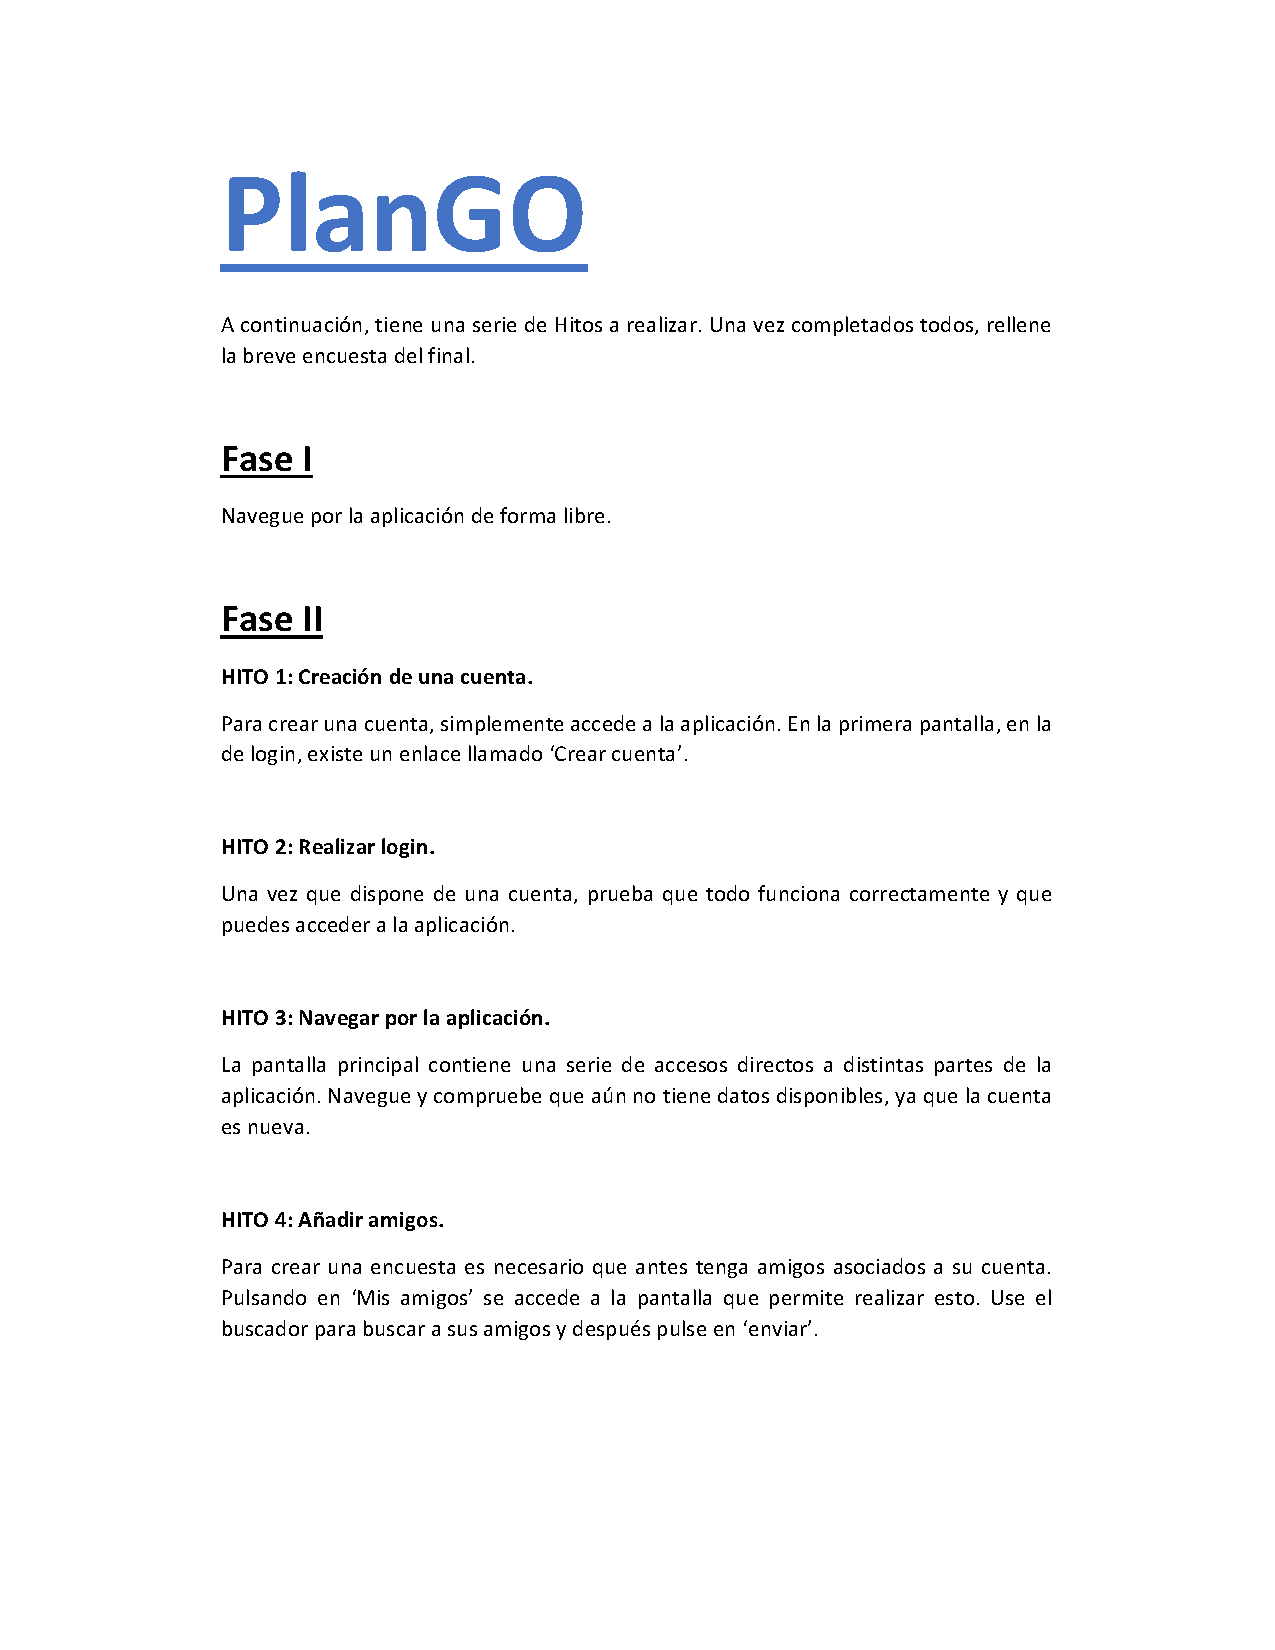
\includepdf[scale=0.9,pages=1,pagecommand=\section{Documento para prueba}]{encuesta}
\includepdf[scale=0.9,pages=2]{encuesta}





%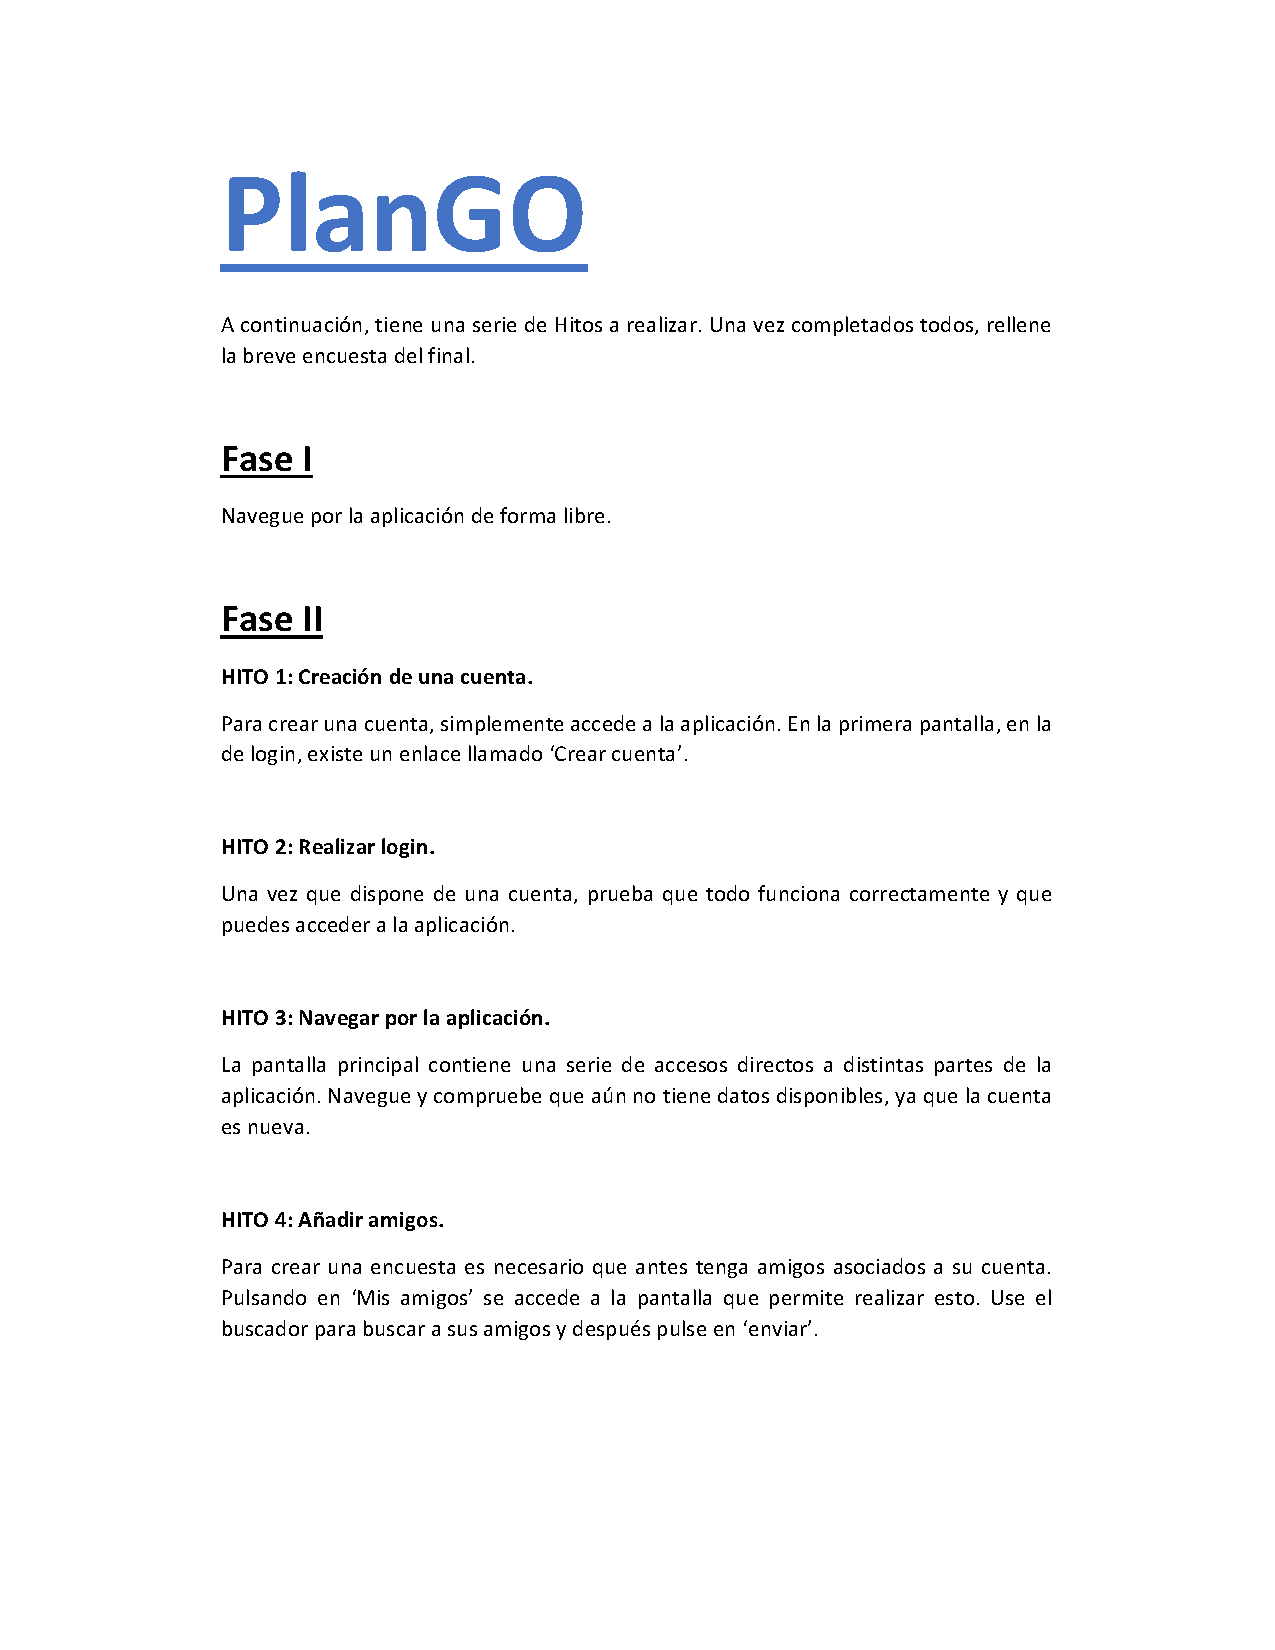
\includegraphics[width=12cm, keepaspectratio]{encuesta.pdf}


%%%%%%%%%%%%%%%%%%%%%%%%%%%%%%%%%%%%%%%%%%%%%%%%%%%%%%%%%%%%%%%%%%%%%%%%%%%%%%%%
%%%%%%%%%%%%%%%%%%%%%%%%%%%%%%%%%%%%%%%%%%%%%%%%%%%%%%%%%%%%%%%%%%%%%%%%%%%%%%%%
% BIBLIOGRAFIA %
%%%%%%%%%%%%%%%%%%%%%%%%%%%%%%%%%%%%%%%%%%%%%%%%%%%%%%%%%%%%%%%%%%%%%%%%%%%%%%%%

\cleardoublepage

% Las siguientes dos instrucciones es todo lo que necesitas
% para incluir las citas en la memoria

\bibliographystyle{plain}
\bibliography{memoria}  % memoria.bib es el nombre del fichero que contiene
% las referencias bibliogr�ficas. Abre ese fichero y mira el formato que tiene,
% que se conoce como BibTeX. Hay muchos sitios que exportan referencias en
% formato BibTeX. Prueba a buscar en http://scholar.google.com por referencias
% y ver�s que lo puedes hacer de manera sencilla.
% M�s informaci�n: 
% http://texblog.org/2014/04/22/using-google-scholar-to-download-bibtex-citations/



\end{document}
